%%%%%%%%%%%%%%%%%%%%%%%%%%%%%%%%%%%%%%%%%
% Beamer Presentation
% LaTeX Template
% Version 2.0 (March 8, 2022)
%
% This template originates from:
% https://www.LaTeXTemplates.com
%
% Author:
% Vel (vel@latextemplates.com)
%
% License:
% CC BY-NC-SA 4.0 (https://creativecommons.org/licenses/by-nc-sa/4.0/)
%
%%%%%%%%%%%%%%%%%%%%%%%%%%%%%%%%%%%%%%%%%

%----------------------------------------------------------------------------------------
%	PACKAGES AND OTHER DOCUMENT CONFIGURATIONS
%----------------------------------------------------------------------------------------

\documentclass[
	11pt, % Set the default font size, options include: 8pt, 9pt, 10pt, 11pt, 12pt, 14pt, 17pt, 20pt
	%t, % Uncomment to vertically align all slide content to the top of the slide, rather than the default centered
	%aspectratio=169, % Uncomment to set the aspect ratio to a 16:9 ratio which matches the aspect ratio of 1080p and 4K screens and projectors
 xcolor={dvipsnames,svgnames}
]{beamer}


\usepackage{graphicx}
\graphicspath{{Images/}{gif folder/}{Figures/}}
\usepackage{eso-pic} % For the background picture on the title page
\usepackage{subfig} % Numbered and caption subfigures using \subfloat
\usepackage{caption} % Coloured captions
\usepackage{transparent}

\usepackage{lmodern}
\usepackage{booktabs}% Allows the use of \toprule, \midrule and \bottomrule for better rules in tables
\usepackage{hyperref}


%----------------------------------------------------------------------------------------
%	SELECT LAYOUT THEME
%----------------------------------------------------------------------------------------

% Beamer comes with a number of default layout themes which change the colors and layouts of slides. Below is a list of all themes available, uncomment each in turn to see what they look like.

%\usetheme{default}
% \usetheme{AnnArbor}
% \usetheme{Antibes}
%\usetheme{Bergen}
% \usetheme{Berkeley}
% \usetheme{Berlin}
%\usetheme{Boadilla}
\usetheme{CambridgeUS}
% \usetheme{Copenhagen}
% \usetheme{Darmstadt}
% \usetheme{Dresden}
% \usetheme{Frankfurt}
%\usetheme{Goettingen}
% \usetheme{Hannover}
%\usetheme{Ilmenau}
%\usetheme{JuanLesPins}
%\usetheme{Luebeck}
% \usetheme{Madrid} % bello
%\usetheme{Malmoe}
%\usetheme{Marburg}
%\usetheme{Montpellier}
% \usetheme{PaloAlto}
%\usetheme{Pittsburgh}
% \usetheme{Rochester}
% \usetheme{Singapore}
% \usetheme{Szeged}
%\usetheme{Warsaw}

%----------------------------------------------------------------------------------------
%	SELECT COLOR THEME
%----------------------------------------------------------------------------------------

% Beamer comes with a number of color themes that can be applied to any layout theme to change its colors. Uncomment each of these in turn to see how they change the colors of your selected layout theme.

%\usecolortheme{albatross}
% \usecolortheme{beaver}
% \usecolortheme{orchid}
% \usecolortheme{beetle}
% \usecolortheme{crane}
%\usecolortheme{dolphin}
%\usecolortheme{dove}
%\usecolortheme{rose}
%\usecolortheme{fly}
%\usecolortheme{lily}
%\usecolortheme{monarca}
%\usecolortheme{seagull}
% \usecolortheme{seahorse}
% \usecolortheme{spruce}
%\usecolortheme{whale}
%\usecolortheme{wolverine}

% \usepackage{xcolor}
\definecolor{darkred}{rgb}{0.8,0,0}
\definecolor{poliBlue}{rgb}{0.102, 0.255, 0.369}
\definecolor{fucsianotes}{RGB}{213, 137, 235}
\definecolor{violanotes}{RGB}{98, 45, 144}

% \definecolor{testcol}{HTML}{4B1D91}
% \definecolor{testcol}{HTML}{7B1299}
% \definecolor{testcol}{HTML}{A0119D}
\definecolor{testcol}{HTML}{DA3A90}
% \definecolor{testcol}{HTML}{ED577C}

% \setbeamercolor{title}{fg=poliBlue}
% \setbeamercolor{frametitle}{fg=poliBlue}
%\setbeamercolor{normal text}{fg=black,bg=white}
%\setbeamercolor{section number projected}{bg=poliBlue}

% \setbeamercolor{palette primary}{fg=black, bg=poliBlue!60!white}
% \setbeamercolor{palette secondary}{fg=black, bg=poliBlue!40!white}
% \setbeamercolor{palette tertiary}{fg=black, bg=poliBlue!20!white}



% \setbeamercolor*{structure}{bg=Thistle!20,fg=Thistle}
% \setbeamercolor*{structure}{bg=WildStrawberry!20,fg=RubineRed}
% \setbeamercolor*{structure}{bg=Periwkinkle!20,fg=Periwkinkle}
% \setbeamercolor*{structure}{bg=WildStrawberry!20,fg=WildStrawberry!20!Plum!50}
% \setbeamercolor*{structure}{bg=DarkOrchid!20,fg=DarkOrchid}
\setbeamercolor*{structure}{bg=RedViolet!20,fg=RedViolet}
% \setbeamercolor*{structure}{bg=Plum!20,fg=Plum}

% \setbeamercolor*{structure}{bg=darkred,fg=poliBlue}
\setbeamercolor*{palette primary}{use=structure,fg=white,bg=structure.fg}
\setbeamercolor*{palette secondary}{use=structure,fg=white,bg=structure.fg!75}
\setbeamercolor*{palette tertiary}{use=structure,fg=white,bg=structure.fg!50!black}
\setbeamercolor*{palette quaternary}{fg=white,bg=black}
\setbeamercolor{section in toc}{fg=black,bg=white}
\setbeamercolor{alerted text}{use=structure,fg=structure.fg!80}
\setbeamercolor{titlelike}{parent=palette primary,fg=structure.fg!50!black}
%%%%%%%%% RedViolet RedViolet RubinedRed
%%%%%%%%% Plum Plum Plum anche

%%%%%%%%%%% non usate
% \setbeamercolor{alerted text}{use=structure,fg=structure.fg!50!black!80!black}
% \setbeamercolor{frametitle}{bg=gray!10!white,fg=Plum}
% \setbeamercolor{frametitle}{bg=gray!10!white,fg=RubineRed!90!black}


% \setbeamercolor*{titlelike}{parent=palette primary}


%----------------------------------------------------------------------------------------
%	SELECT FONT THEME & FONTS
%----------------------------------------------------------------------------------------

% Beamer comes with several font themes to easily change the fonts used in various parts of the presentation. Review the comments beside each one to decide if you would like to use it. Note that additional options can be specified for several of these font themes, consult the beamer documentation for more information.

\usefonttheme{default} % Typeset using the default sans serif font
%\usefonttheme{serif} % Typeset using the default serif font (make sure a sans font isn't being set as the default font if you use this option!)
%\usefonttheme{structurebold} % Typeset important structure text (titles, headlines, footlines, sidebar, etc) in bold
%\usefonttheme{structureitalicserif} % Typeset important structure text (titles, headlines, footlines, sidebar, etc) in italic serif
%\usefonttheme{structuresmallcapsserif} % Typeset important structure text (titles, headlines, footlines, sidebar, etc) in small caps serif

%------------------------------------------------

%\usepackage{mathptmx} % Use the Times font for serif text
%\usepackage{palatino} % Use the Palatino font for serif text

%\usepackage{helvet} % Use the Helvetica font for sans serif text
%\usepackage[default]{opensans} % Use the Open Sans font for sans serif text
%\usepackage[default]{FiraSans} % Use the Fira Sans font for sans serif text
%\usepackage[default]{lato} % Use the Lato font for sans serif text

%----------------------------------------------------------------------------------------
%	SELECT INNER THEME
%----------------------------------------------------------------------------------------

% Inner themes change the styling of internal slide elements, for example: bullet points, blocks, bibliography entries, title pages, theorems, etc. Uncomment each theme in turn to see what changes it makes to your presentation.

%\useinnertheme{default}
\useinnertheme{circles}
%\useinnertheme{rectangles}
%\useinnertheme{rounded}
%\useinnertheme{inmargin}

%----------------------------------------------------------------------------------------
%	SELECT OUTER THEME
%----------------------------------------------------------------------------------------

% Outer themes change the overall layout of slides, such as: header and footer lines, sidebars and slide titles. Uncomment each theme in turn to see what changes it makes to your presentation.

%\useoutertheme{default}
% \useoutertheme{infolines}
%\useoutertheme{miniframes}
% \useoutertheme{smoothbars}
% \useoutertheme{sidebar}
% \useoutertheme{split}
% \useoutertheme{shadow}
% \useoutertheme{tree}
% \useoutertheme{smoothtree}


%\setbeamertemplate{footline} % Uncomment this line to remove the footer line in all slides
%\setbeamertemplate{footline}[page number] % Uncomment this line to replace the footer line in all slides with a simple slide count

\setbeamertemplate{navigation symbols}{} % Uncomment this line to remove the navigation symbols from the bottom of all slides

%----------------------------------------------------------------------------------------
%	PRESENTATION INFORMATION
%----------------------------------------------------------------------------------------

% \title[DRPM revision]{Back to business}
% The DRPM Strikes Back
\title[]{The DRPM Strikes Back: More Flexibility for a Bayesian Spatio-Temporal Clustering Model
}
% The short title in the optional parameter appears at the bottom of every slide, the full title in the main parameter is only on the title page

\subtitle{} % Presentation subtitle, remove this command if a subtitle isn't required


\author[]{\texorpdfstring{%
\footnotesize 
\begin{minipage}{.4\textwidth}
\centering
Candidate: Federico Angelo Mor
\end{minipage}%  
\begin{minipage}{.5\textwidth}
\centering
Advisor: Prof. Alessandra Guglielmi\\
Coadvisor: Prof. Alessandro Carminati
\end{minipage}}{The Author}}
% \author[]{\small Candidate: Federico Angelo Mor\\Advisor: Prof. Alessandra Guglielmi\\Coadvisor: Prof. Alessandro Carminati} % Presenter name(s), the optional parameter can contain a shortened version to appear on the bottom of every slide, while the main parameter will appear on the title slide

\institute[]{
\vspace{-10pt}
\begin{figure}
    \centering
    
\includegraphics[width=0.47\linewidth]{Immagini/polimi2.pdf}
\end{figure}\vspace{-10pt}
% Politecnico di Milano
	% Politecnico of Milano\\% \smallskip 
	%\textit{james@LaTeXTemplates.com}
} % Your institution, the optional parameter can be used for the institution shorthand and will appear on the bottom of every slide after author names, while the required parameter is used on the title slide and can include your email address or additional information on separate lines

% \author[]{Federico}

\date[]{
% \today
December 11, 2024
}

% May 30, 2024
% eventually in May%\\[4pt]
% \scriptsize{
% % \tiny{
% github project repository: \url{https://github.com/federicomor/progetto-bayesian} \\
% visualization page: \url{https://federicomor.github.io/assets/figures/visualize.html}
% }
% }
% Presentation date or conference/meeting name, the optional parameter can contain a shortened version to appear on the bottom of every slide, while the required parameter value is output to the title slide

\usepackage{amsmath}

\newcommand{\iter}{ \text{iter}}
\newcommand{\fit}{ \text{fit}}
\newcommand{\op}[1]{\operatorname{#1}}

\renewcommand{\tt}{\texttt}
\renewcommand{\sf}{\textsf}


%%% Math stuff
\usepackage{bm}
\renewcommand{\vec}{\boldsymbol}
\DeclareMathOperator{\diag}{diag}
\DeclareMathOperator{\var}{var}
\newcommand{\simind}{\overset{\text{ind}}{\sim}}
\newcommand{\simiid}{\overset{\text{iid}}{\sim}}
\renewcommand{\P}{\mathbb{P}}
\newcommand{\E}{\mathbb{E}}
\newcommand{\G}{\mathcal{G}}
\newcommand{\N}{\mathcal{N}}
\newcommand{\Ncan}{\mathcal{N}\text{Canon}}
\newcommand{\U}{\mathcal{U}}
\newcommand{\invgamma}{\text{invGamma}}
\newcommand{\Beta}{\text{Beta}}
\newcommand{\Ber}{\text{Ber}}
\newcommand{\csi}{\xi}

\newcommand{\indicator}[1]{\mathbbm{1}_{[#1]}}
% \newcommand{\indicator}[1]{\mathbbm{1}{#1}}

\renewcommand{\L}{\mathcal{L}}
\newcommand{\law}{\mathcal{L}}
% \newcommand{\law}{\mathfrak{L}}
\newcommand{\ari}{\operatorname{ARI}}
\newcommand{\ARI}{\operatorname{ARI}}
\renewcommand{\ln}{\operatorname{ln}}
\newcommand{\post}{\text{(post)}}
\newcommand{\postp}[1]{#1\text{(post)}}
\newcommand{\expp}[1]{ \exp \left\{ #1 \right\} }


\newcommand{\blue}[1]{\textcolor{blue}{#1}}
\newcommand{\magenta}[1]{\textcolor{magenta}{#1}}
\newcommand{\gray}[1]{\textcolor{gray}{#1}}
\newcommand{\alert}[1]{\textcolor{RedViolet}{#1}}
\newcommand{\alertg}[1]{\textcolor{Violet!65!Black}{#1}}
\newcommand{\galert}[1]{\textcolor{Violet!65!Black}{#1}}

\AtBeginSection[]
{
\setbeamercolor{section in toc}{fg=alerted text.fg}
\setbeamercolor{section in toc shaded}{fg=black}
\begin{frame}<beamer>
  % \frametitle{Outline}
\tableofcontents[currentsection,currentsubsection,subsectionstyle=show/shaded/hide, hideothersubsections]
\end{frame}
}


% \AtBeginSubsection[]
% {
% \setbeamercolor{section in toc}{fg=alerted text.fg}
% \setbeamercolor{section in toc shaded}{fg=black}
% \begin{frame}<beamer>
%   % \frametitle{Outline}
% \tableofcontents[currentsection,currentsubsection,subsectionstyle=show/shaded/hide, hideothersubsections]
% \end{frame}
% }

% \newcommand{\cmark}{\textcolor[RGB]{100, 200, 100}{\ding{51}}}%
% \newcommand{\xmark}{\textcolor[RGB]{200, 100, 100}{\ding{55}}}%
\newcommand{\cmark}{\textcolor[RGB]{58, 119, 186}{\ding{51}}}%
\newcommand{\xmark}{\textcolor[RGB]{190, 206, 220}{\ding{55}}}%

%%% Project stuff
\newcommand{\pmten}{\ensuremath\text{PM}_{10}} 

%%% Gif stuff not nec in the report
% \usepackage{multimedia}
% \usepackage{animate}
% \usepackage{xmpmulti}
\usepackage{multirow}
\usepackage{todonotes}

\newcommand{\mcal}[1]{\mathcal{#1}}

% \newenvironment{captioning}[1][0]{\begin{minipage}{0.6/textwidth}}{\end{minipage}}
\newenvironment{captioning}
    {
    \begin{minipage}{0.9\textwidth}
    \centering
    }
    {
    \end{minipage}
    }

\renewcommand{\epsilon}{\varepsilon}
\renewcommand{\theta}{\vartheta}
% \renewcommand{\rho}{\varrho}
\renewcommand{\phi}{\varphi}

%----------------------------------------------------------------------------------------

% \usepackage{bm}

% \renewcommand{\red}[1]{\textcolor{darkred}{#1}}
\definecolor{linkBlue}{RGB}{100,80,150}
% \newcommand{\blue}[1]{\textcolor{poliBlue}{#1}}
% \newcommand{\blue}[1]{\textcolor{linkBlue}{#1}}
% \definecolor{pink}{RGB}{230,180,200}
\definecolor{pink}{RGB}{200,190,230}
\newcommand{\pink}[1]{\textcolor{pink}{\small #1}}

% \setbeamercolor{alerted text}{fg=darkred}


% \usepackage{multimedia}
% \usepackage{animate}
% \usepackage{xmpmulti}
\usepackage{pbox}

\usepackage{tikz}
\usetikzlibrary{arrows.meta, positioning}

\usepackage[
% maxbibnames=99,
% minbibnames=1,
maxcitenames=1,
% mincitenames=1,
style=authoryear,
uniquelist=false,
hyperref, % riferimenti cliccabili
backref, % link alle pagine in cui il riferimento è citato
natbib, % mantiene compatibilità con eventuali comandi natbib
backend=biber, % motore bibliografico (v. ArteLatex di Pantieri)
defernumbers=false,	% riferimenti ordinati in ordine di comparsa
sorting=nty
]{biblatex}\addbibresource{Bibliografia.bib}	% database bibliografico
\let\cite\citep

%\usepackage{emoji}
%\newcommand{\temoji}[1]{\tiny{\emoji{#1}}}
%\newcommand{\semoji}[1]{\small{\emoji{#1}}}
%\newcommand{\femoji}[1]{\footnotesize{\emoji{#1}}}
\newcommand{\balert}[1]{\textbf{\alert{#1}}}
\newcommand\numberthis{\addtocounter{equation}{1}\tag{\theequation}}
\usepackage{svg}

\usepackage[autostyle, english = american]{csquotes}
\MakeOuterQuote{"} % prettier quotes/virgolette, "

\usepackage{minted}
\newcommand{\mjline}[1]{\mintinline{julia}{#1}}
\usemintedstyle{friendly}
\newenvironment{code}{\captionsetup{type=listing}}{}

\captionsetup{tableposition=top,
	figureposition=bottom,
	font=footnotesize,
	% font=small,
	% format=hang,
	% labelfont={bf,sc}
	% labelfont=bf
        % labelfont={color=bluePoli}
        }


\setbeamertemplate{blocks}[framed]
% 1- Block title (background and text)
\setbeamercolor{block title}{bg=cyan, fg=white}
% 2- Block body (background)
\definecolor{LightLilac}{RGB}{235, 224, 245}
\definecolor{PalePink}{RGB}{255, 228, 240}
\definecolor{LightGrayBlue}{RGB}{220, 230, 240}
\definecolor{MutedPurple}{RGB}{200, 180, 230}
\definecolor{SoftCoral}{RGB}{250, 210, 200}
% \setbeamercolor{block body}{bg=MutedPurple}

% \definecolor{newcol}{RGB}{189, 91, 165}
% \definecolor{newcol}{RGB}{138, 66, 125}
% \definecolor{newcol}{RGB}{158, 148, 164}
\definecolor{newcol}{RGB}{194, 182, 202}
% \definecolor{newcol}{RGB}{204,189,189}
% \definecolor{newcol}{RGB}{229,206,206}
% \setbeamercolor{block body}{bg=newcol!30}
% \setbeamercolor{block body}{bg=Thistle!10}
% \setbeamercolor{block body}{bg=WildStrawberry!10}
\setbeamercolor{block body}{bg=Purple!14!Gray!10}

     \setbeamertemplate{footline}
        {
      \leavevmode%
      \hbox{%
      \begin{beamercolorbox}[wd=.333333\paperwidth,ht=2.25ex,dp=1ex,center]{author in head/foot}%
        \usebeamerfont{author in head/foot}\insertshortauthor~~\insertshortinstitute
      \end{beamercolorbox}%
      \begin{beamercolorbox}[wd=.333333\paperwidth,ht=2.25ex,dp=1ex,center]{title in head/foot}%
        \usebeamerfont{title in head/foot}\insertshorttitle
      \end{beamercolorbox}%
      \begin{beamercolorbox}[wd=.333333\paperwidth,ht=2.25ex,dp=1ex,right]{date in head/foot}%
        \usebeamerfont{date in head/foot}\insertshortdate{}\hspace*{2em}

    %#turning the next line into a comment, erases the frame numbers
        % \insertframenumber{} / \inserttotalframenumber\hspace*{2ex} 
        \insertframenumber{}\hspace*{2ex} 

      \end{beamercolorbox}}%
      \vskip0pt%
    }

\setbeamercovered{dynamic}
% \setbeamercovered{transparent}
% \usepackage{enumitem}
\usepackage{multicol}
\usepackage{onimage}
\begin{document}


%----------------------------------------------------------------------------------------
%	TITLE SLIDE
%----------------------------------------------------------------------------------------

% { % all template changes are local to this group.
%     \setbeamertemplate{navigation symbols}{}
%     \begin{frame}<article:0>[plain]
%         \begin{tikzpicture}[remember picture,overlay]
%             \node[at=(current page.center)] {
%                 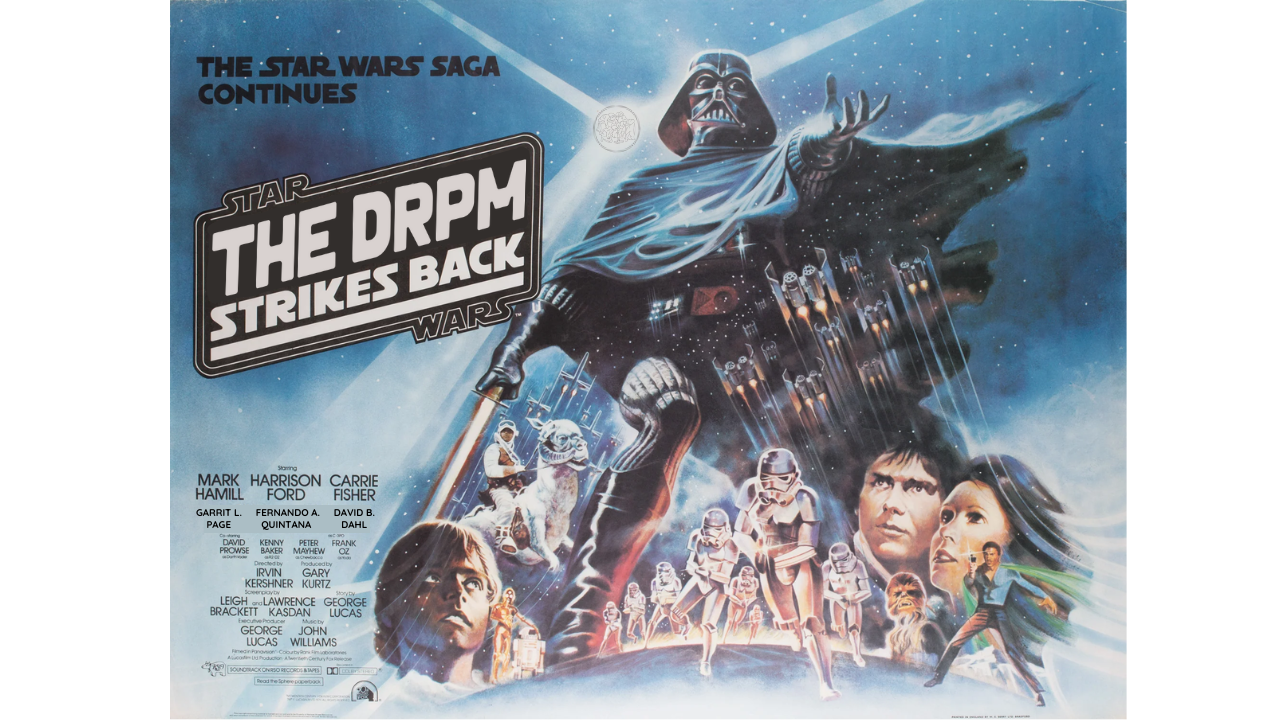
\includegraphics[keepaspectratio,
%                                  width =1.37\paperwidth,
%                                  % height=1.37\paperheight]{imgs/THE DRPM.png}
%                                  height=1.37\paperheight]{imgs/THE DRPM.pdf}
%             };
%         \end{tikzpicture}
%      \end{frame}
% }


\begin{frame}
	\titlepage % Output the title slide, automatically created using the text entered in the PRESENTATION INFORMATION block above
 
\end{frame}

%----------------------------------------------------------------------------------------
%	TABLE OF CONTENTS SLIDE
%----------------------------------------------------------------------------------------

% The table of contents outputs the sections and subsections that appear in your presentation, specified with the standard \section and \subsection commands. You may either display all sections and subsections on one slide with \tableofcontents, or display each section at a time on subsequent slides with \tableofcontents[pausesections]. The latter is useful if you want to step through each section and mention what you will discuss.


\begin{frame}{What is the thesis about?}

\begin{block}{}
The Dependent Random Partition Model from \cite{1-drpm} is a Bayesian spatio-temporal clustering model which directly models the dependencies in the sequence of clusters over time.\\[6pt]
\end{block}
% \vspace{10pt}
Currently, the model
\begin{itemize}
\item produces up to spatially-informed clusters \\\phantom{\alert{$\to$ I additionally introduced covariates information}}
\item only accepts complete datasets \\\phantom{\alert{$\to$ I made it work with missing values in the target variable}}
\item has quite slow execution times (especially on large datasets) \\\phantom{\alert{$\to$ I developed a brand-new and more efficient implementation}}
\end{itemize}
\end{frame}

\begin{frame}{What is the thesis about?}

\begin{block}{}
The Dependent Random Partition Model from \cite{1-drpm} is a Bayesian spatio-temporal clustering model which directly models the dependencies in the sequence of clusters over time.\\[6pt]
\end{block}
% \vspace{10pt}
Currently, the model
\begin{itemize}
\item produces up to spatially-informed clusters \\\alert{$\to$ I additionally introduced covariates information}
\item only accepts complete datasets \\\alert{$\to$ I made it work with missing values in the target variable}
\item has quite slow execution times (especially on large datasets) \\\alert{$\to$ I developed a brand-new and more efficient implementation}
\end{itemize}
\end{frame}

% \begin{minipage}{.5\textwidth}
% The current implementation:
%   \begin{itemize}
% \item produces up to spatially-informed clusters
% \item only accepts complete datasets 
% \item has quite slow execution times  
% \end{itemize}
% \end{minipage}% This must go next to `\end{minipage}`
% \begin{minipage}{.5\textwidth}
% \alert{Our generalization:}
%   \begin{itemize}
% \item \alert{additionally includes covariates information}
% \item \alert{works with missing values}
% \item \alert{provides faster execution times} 
% \end{itemize}
% \end{minipage}


% \begin{frame}{Contents}
% 	% \frametitle{Contents}
% 	%Overview Outline Summary, choose a synonym}
% 	% Slide title, remove this command for no title
% 	\tableofcontents % Output the table of contents (all sections on one slide)
% 	%\tableofcontents[pausesections] % Output the table of contents (break sections up across separate slides)
% \end{frame}

% \begin{frame}{Contents}
% \begin{enumerate}
%     \item \balert{Introduction}\\
%     Methods for clustering\\[10pt]
%     \item Description of the model(s)
%     \item Implementation and optimizations
%     \item Analysis of the models
%     \item Conclusion
% \end{enumerate}\end{frame}

% Presentation structure
% - Summary (1 slide – can also be dropped)
% - Faced problem and goals (1-2 slides)
% - State of art (1 slide)
% - Approach to the problem solution (2-5 slides)
% - Software architecture (1 slide)
% - Obtained Results (3-5 slides)
% - Conclusions (1 slide)

% ==============================================
\section{Description of the problem}
\subsection{What is the DRPM}

% \begin{frame}{What is the DRPM? more in detail}
\begin{frame}{Clustering}

% The Dependent Random Partition Model from \cite{1-drpm} is a Bayesian spatio-temporal \alert{clustering} model which \textit{directly} models the dependencies in the sequence of clusters over time.\\[6pt]
\begin{block}{}
The Dependent Random Partition Model from \cite{1-drpm} is a Bayesian spatio-temporal \alert{clustering} model which directly models the temporal dependencies in the sequence of clusters over time.\\[6pt]
\end{block}
Clustering is a fundamental technique of unsupervised learning where a set of data points has to be divided into homogeneous groups of units which exhibit a similar behaviour.
\begin{figure}
    \centering
    % \fbox{
    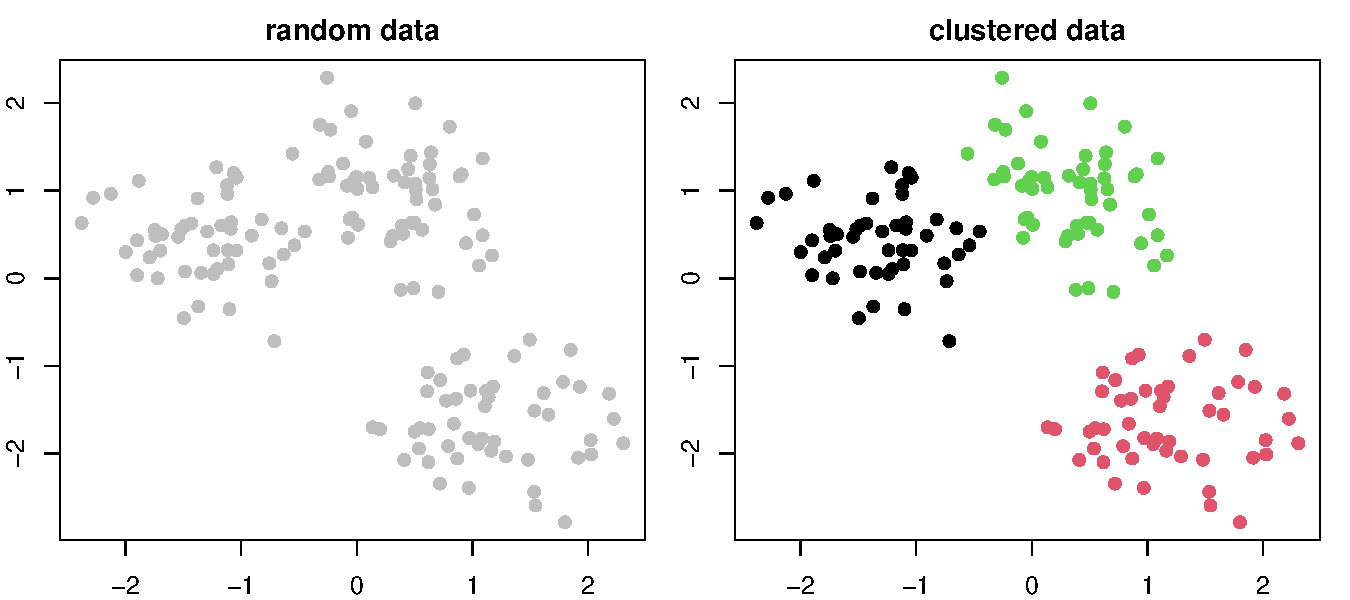
\includegraphics[clip,trim=2px 0px 2px 22px, width=0.76\linewidth]{imgs/example_clusters.pdf}
    % }
\end{figure}
\end{frame}


% \begin{frame}{What is the DRPM? more in detail}
\begin{frame}{Why going Bayesian?}

\begin{block}{}
The Dependent Random Partition Model from \cite{1-drpm} is a \alert{Bayesian} spatio-temporal clustering \alert{model} which directly models the temporal dependencies in the sequence of clusters over time.\\[6pt]
\end{block}
Bayesian models incorporate prior information on the model 
parameters and allow to assess uncertainty when performing inference on the results. 
% This is achieved by treating each model parameter as a random variable with a corresponding prior distribution.
\begin{figure}
    \centering
    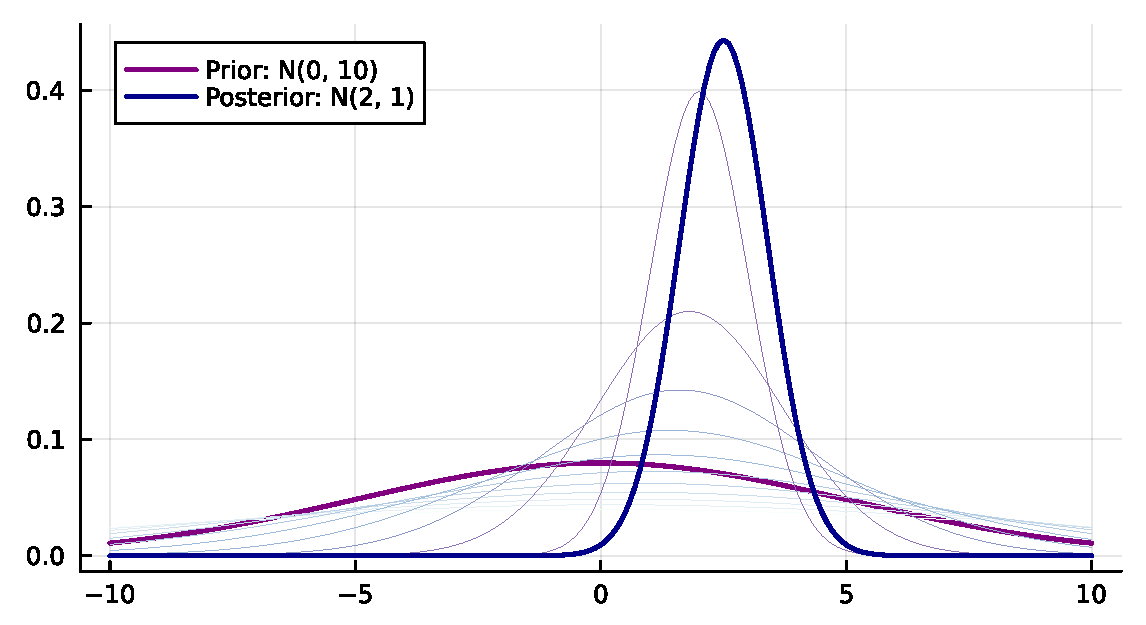
\includegraphics[width=0.68\linewidth]{imgs/prior_post.pdf}
    % \caption{Enter Caption}
    \label{fig:enter-label}
\end{figure}
\end{frame}

% \begin{frame}{What is the DRPM? more in detail}
\begin{frame}{A bit of (spatio-temporal) context}

\begin{block}{}
The Dependent Random Partition Model from \cite{1-drpm} is a Bayesian \alert{spatio-temporal} clustering model which directly models the temporal dependencies in the sequence of clusters over time.\\[6pt]
\end{block}
In spatio-temporal datasets, observations are collected over time and across various spatial locations.
% is inherently complex due to the interplay between spatial and temporal dimensions; a complexity that is further compounded when covariates are also available.
So we will have $n$ units that have to be clustered at all time instants $t=1,\ldots,T$. 
% Each unit is represented as $i=1,\ldots,n$. We denote by $\rho_t=\{S_{1t}, \ldots, S_{k_tt}\}$ the partition at time $t$ of the $n$ experimental units, composed by $k_t$ clusters. An alternative representation of this partition is possible through cluster labels $\vec{c}_t = \{ c_{1t}, \ldots, c_{nt}\}$, with $c_{it}=j$ indicating that unit $i$ belongs to cluster $S_{jt}$. 
\begin{figure}
    \centering
    % \fbox{
    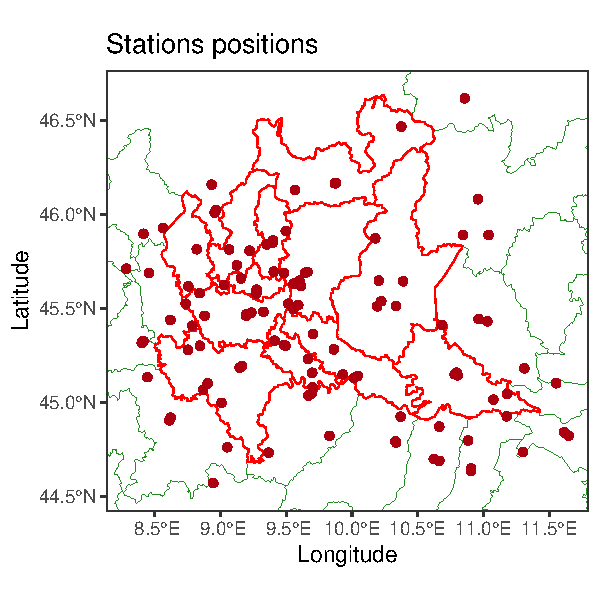
\includegraphics[clip,trim=18px 26px 5px 29px, 
    % width=0.28\linewidth]{imgs/stations_map_only_dots.pdf}
    width=0.32\linewidth]{imgs/map_dots.pdf}
    % }
    % \fbox{
    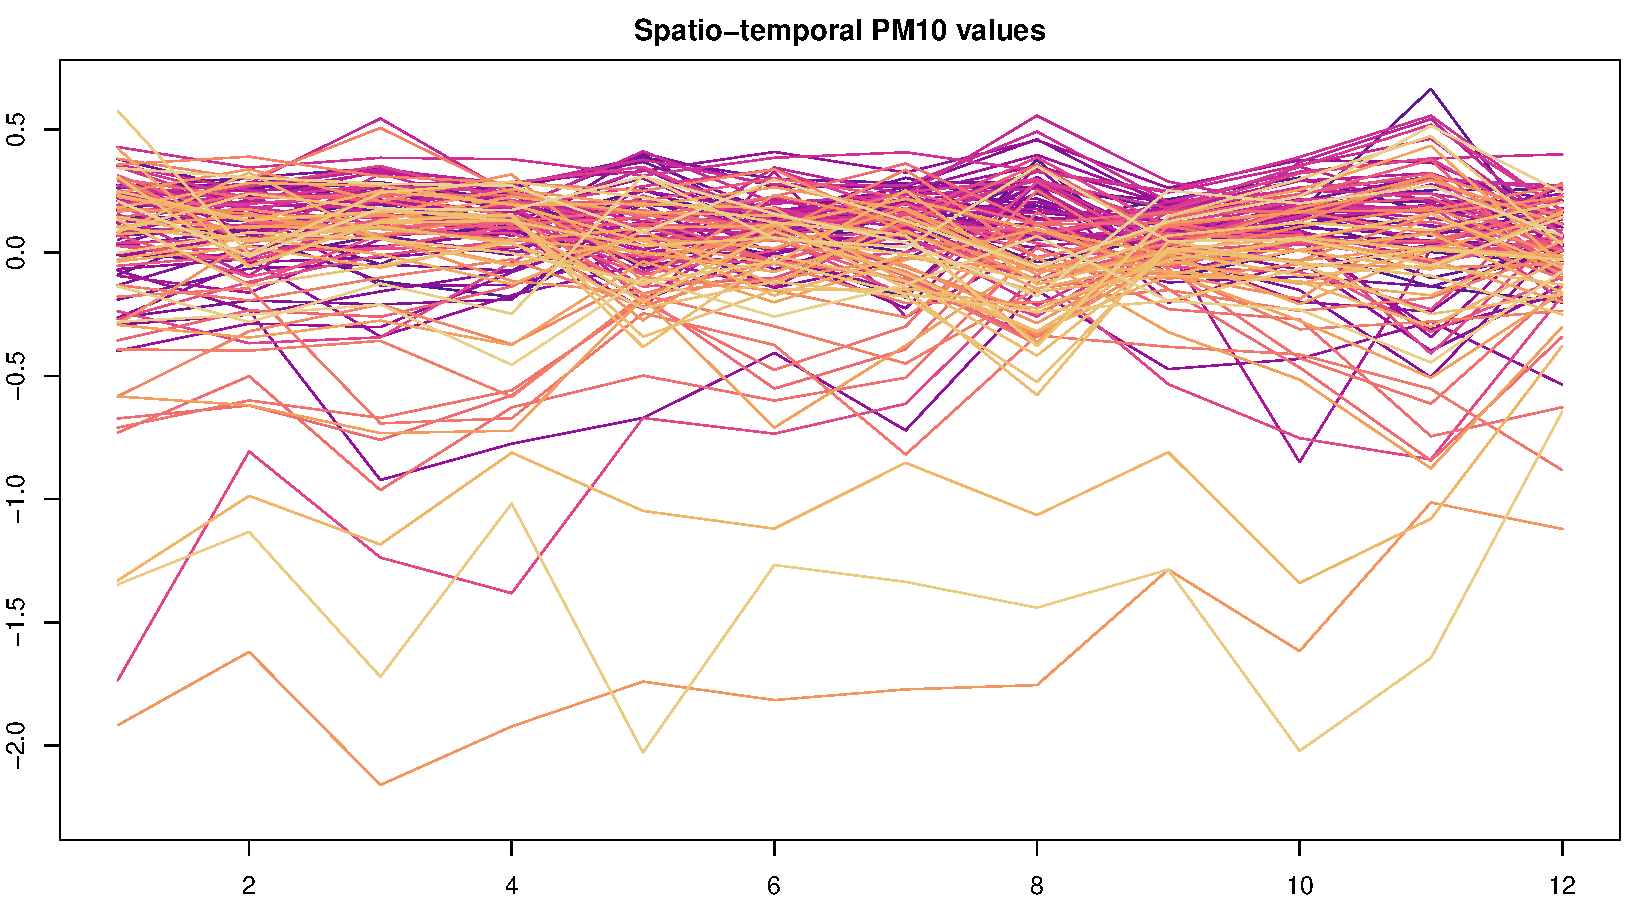
\includegraphics[clip, trim=0px 0px 0px 22px, width=0.54\linewidth]{imgs/test_2_spatial_data.pdf}
    % }
    \label{fig:enter-label}
\end{figure}

% Finally, we will denote with a $\star$ superscript all the variables or quantities which are cluster-specific.
\end{frame}




% \begin{frame}{The real details}
% \begin{frame}{Why temporal dependencies are important?}
\begin{frame}{Why should we care about temporal dependencies?}

\begin{block}{}
The \alert{Dependent} Random Partition Model from \cite{1-drpm} is a Bayesian spatio-temporal clustering model which        \alert{directly models the temporal dependencies in the sequence of clusters over time.}
\end{block}
This allows to derive a more gentle and interpretable evolution of clusters.
% IMMAGINE ARI VARI MODELLI
\begin{figure}
    \centering
    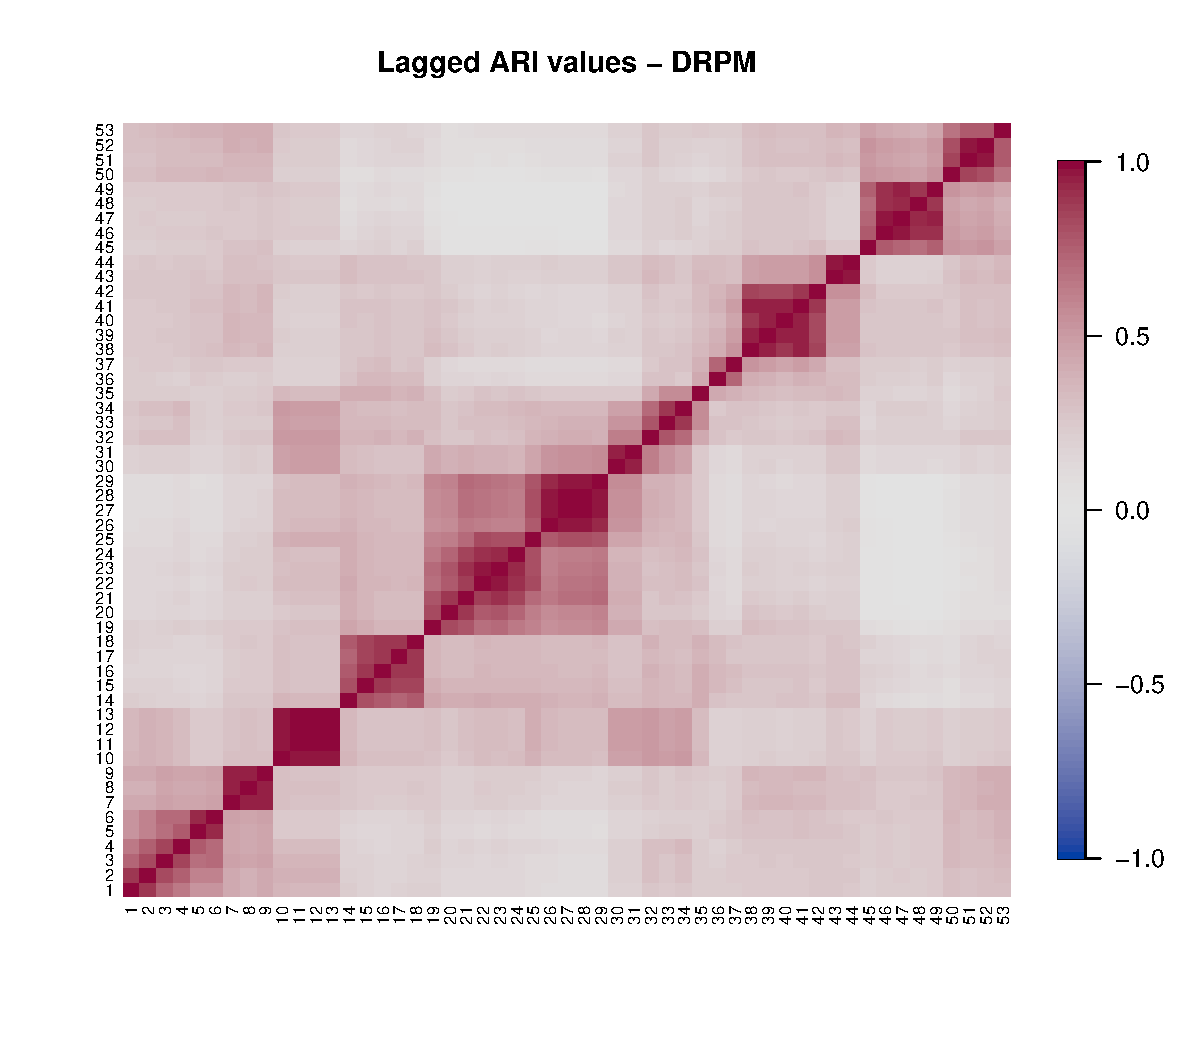
\includegraphics[clip,trim=50px 60px 17px 24px, width=0.45\linewidth]{imgs/ari_drpm.pdf}
    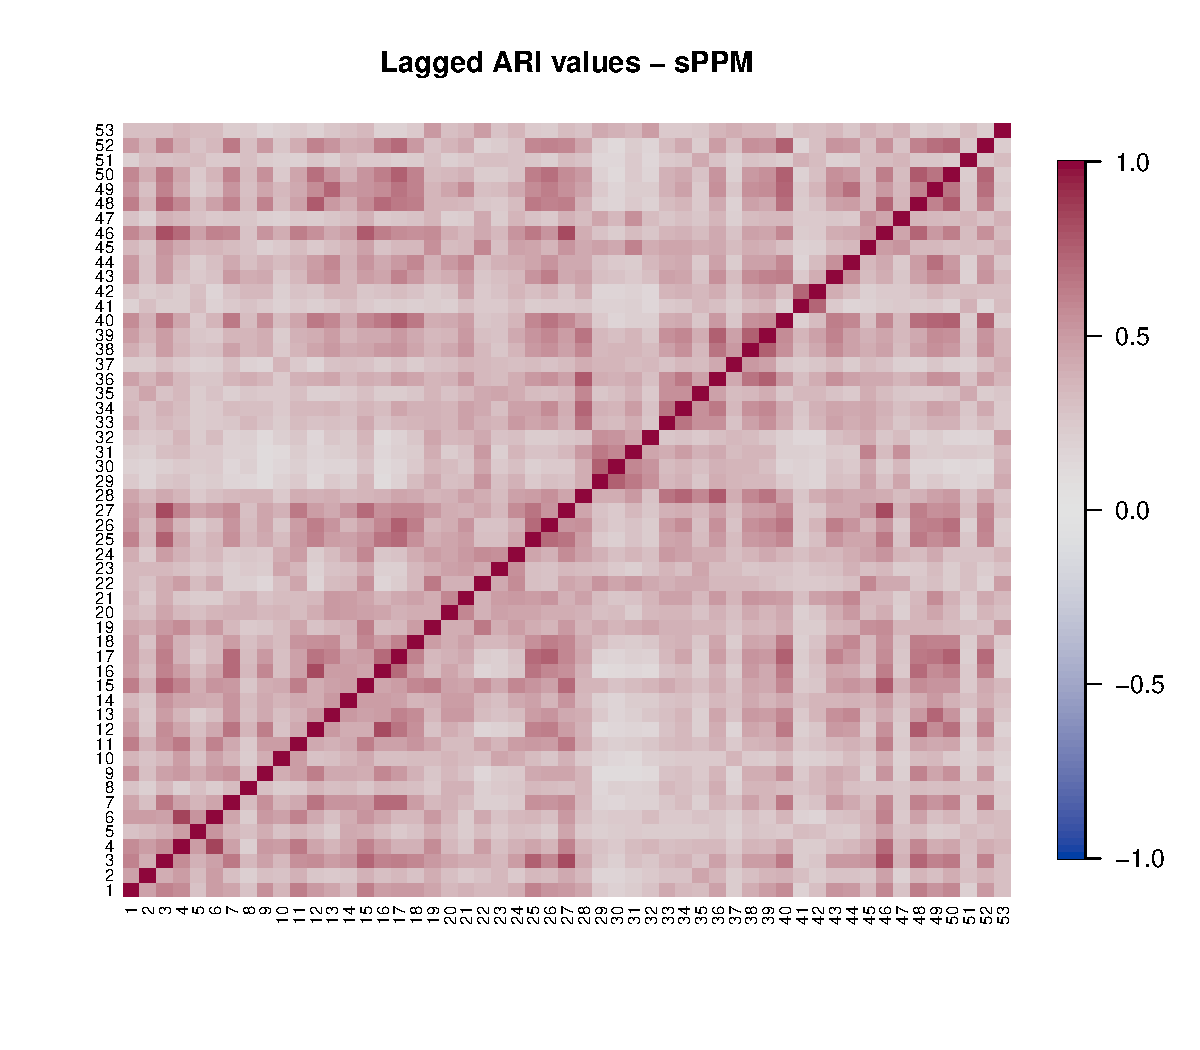
\includegraphics[clip,trim=50px 60px 17px 24px, width=0.45\linewidth]{imgs/ari_sppm.pdf}
\end{figure}
% In spatio-temporal datasets, observations are collected over time and across various spatial locations.
% is inherently complex due to the interplay between spatial and temporal dimensions; a complexity that is further compounded when covariates are also available.
\end{frame}

% \begin{frame}{The real details}
% \begin{frame}{Why temporal dependencies are important?}
\begin{frame}{Why should we care about temporal dependencies?}

\begin{block}{}
The \alert{Dependent} Random Partition Model from \cite{1-drpm} is a Bayesian spatio-temporal clustering model which        \alert{directly models the temporal dependencies in the sequence of clusters over time.}
\end{block}
This allows to derive a more gentle and interpretable evolution of clusters.
% Accounting for temporal dependencies allows to derive a more gentle and interpretable evolution of clusters over time.
% IMMAGINE ARI VARI MODELLI
\begin{figure}
    \centering
    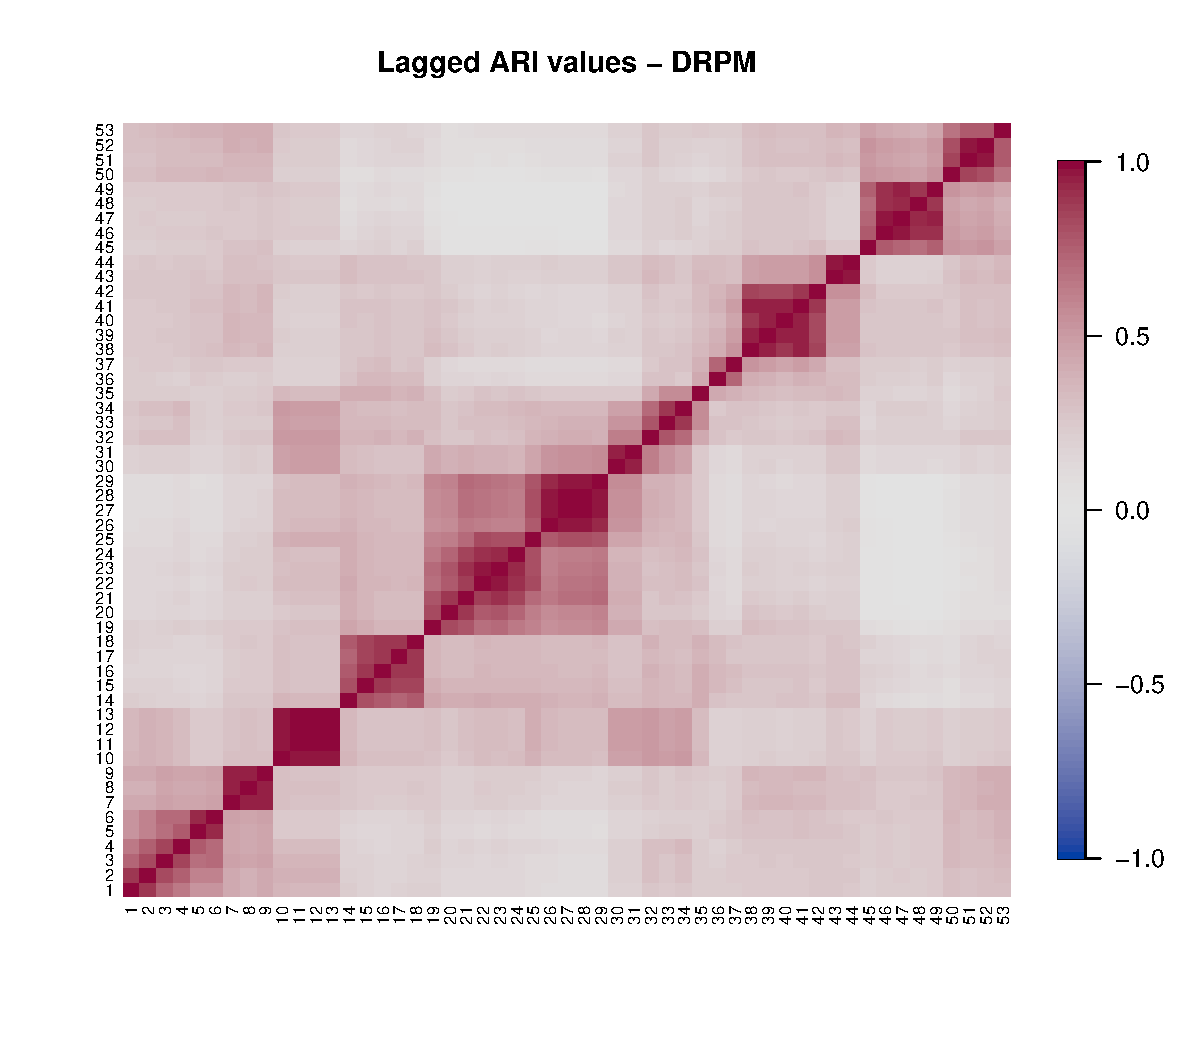
\includegraphics[clip,trim=50px 60px 17px 24px, width=0.45\linewidth]{imgs/ari_drpm.pdf}
    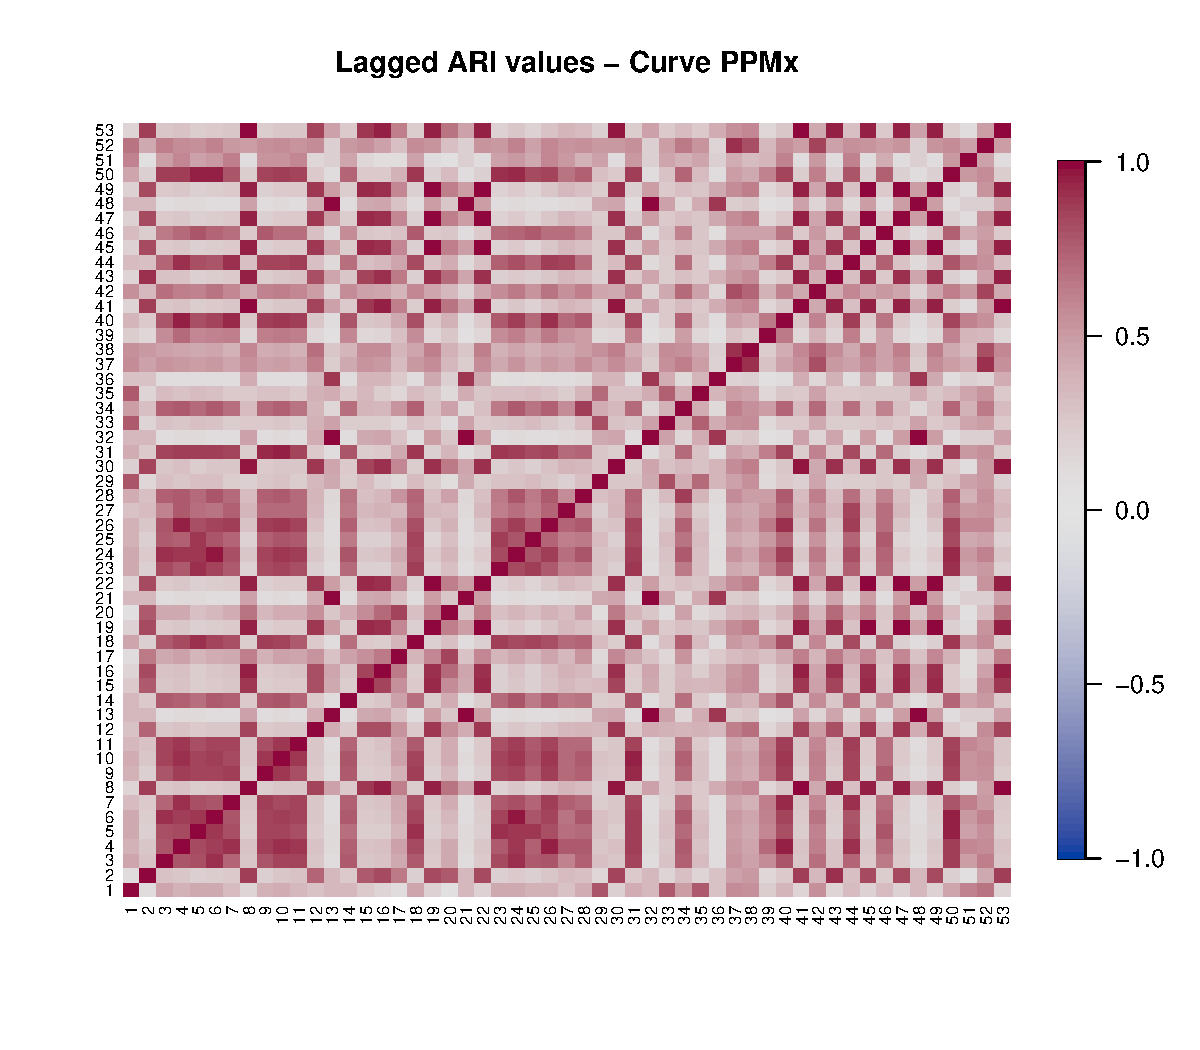
\includegraphics[clip,trim=50px 60px 17px 24px, width=0.45\linewidth]{imgs/ari_curveppmx.pdf}
\end{figure}
% In spatio-temporal datasets, observations are collected over time and across various spatial locations.
% is inherently complex due to the interplay between spatial and temporal dimensions; a complexity that is further compounded when covariates are also available.
\end{frame}


\begin{frame}{Modelling the temporal dependence}
Introducing temporal dependence in a collection of partitions requires the formulation of a joint probability model for $(\rho_1, \ldots, \rho_T)$. \citet{1-drpm} modelled this temporal connection as a first-order Markovian structure, where the conditional distribution of $\rho_t$ given all the predecessors $\rho_{t-1}, \rho_{t-2}, \ldots, \rho_1$ actually depends only on $\rho_{t-1}$, leading to 
% the construction of the joint probability model for $(\rho_1, \ldots, \rho_T)$ as
\begin{equation}
P(\rho_1, \ldots, \rho_T) = P(\rho_T|\rho_{T-1}) \cdots P(\rho_2|\rho_1) P(\rho_1)
\label{P rhos 1}
\end{equation}
Here, $P(\rho_1)$ is an exchangeable partition probability function (EPPF), which describes how the $n$ experimental units at time period 1 are grouped into $k_1$ distinct clusters. \citet{1-drpm} chose this EPPF to be $P(\rho_1) \propto \prod_{j=1}^{k_1} M\cdot(|S_{j1}|-1)! $.
% A commonly encountered EPPF is that induced by a Dirichlet process, implemented by \cite{1-drpm} through a Chinese restaurant process (CRP) 

% \cite{sample-size-consistency}. 
% The EPPF used is given by the following product partition model (PPM) structure
% \begin{equation}
%     % P(\rho_1|M) = \frac{M^{k_1}}{\prod_{i=1}^n (M+i-1)} \prod_{j=1}^{k_1} (|S_j|-1)!
%     P(\rho_1|M) \propto \prod_{j=1}^{k_1} M\cdot(|S_{j1}|-1)!
%     \label{eppf rho1}
% \end{equation}
% where $k_1$ denotes the number of clusters in $\rho_1$, $|S_{j1}|$ is the cardinality of cluster $S_{j1}$, and $M$ is a concentration parameter that controls the number of clusters. 
\end{frame}

\begin{frame}{Modelling the temporal dependence}
    
To characterize the other terms $P(\rho_t|\rho_{t-1})$ in \eqref{P rhos 1}, i.e. to explicitly model how $\rho_{t-1}$ influences $\rho_t$, the following auxiliary variables need to be introduced to. For all units $i=1,\ldots,n$ we define
% Here $P(\rho_1)$ is an exchangeable partition probability function (EPPF) that describes how the $n$ experimental units at time period 1 are grouped into $k_1$ distinct groups. A commonly encountered EPPF is that induced by a Dirichlet process which in \cite{1-drpm} is implemented through a Chinese restaurant process (CRP) \cite{sample-size-consistency}. 
\begin{equation*}
% \gamma_{it} = \begin{cases}
%     1 & \parbox{5.2cm}{if unit $i$ is \emph{not} reallocated when moving from time $t-1$ to $t$} \\
%     0 & \parbox{5.2cm}{otherwise }
% \end{cases}
\gamma_{it} = \begin{cases}
    1 & \text{if unit $i$ is \emph{not} reallocated when moving from time $t-1$ to $t$} \\
    0 & \text{otherwise (namely, the unit \emph{is} reallocated)}
\end{cases}
\end{equation*}
These parameters model the similarity between $\rho_{t-1}$ and $\rho_t$: 
\begin{itemize}
    \item if $\rho_{t-1}$ and $\rho_{t}$ are highly dependent, their cluster configurations will change minimally $\implies$ the majority of $\gamma_{it}$ will be 1
    \item if $\rho_{t-1}$ and $\rho_{t}$ exhibit low dependence, their cluster configurations will change significantly $\implies$ the majority of $\gamma_{it}$ will be 0
\end{itemize}
\end{frame}

\begin{frame}{Modelling the temporal dependence}
    % By construction, we set $\gamma_{i1}=0$ for all $i$, meaning that at the first time instant all units will get reallocated since there is no partition at time $t=0$. 
\citet{1-drpm} assumed $\gamma_{it} \mathrel{\raisebox{-2pt}{$\simind$}} \Ber(\alpha_t)$, where $\alpha_t \in [0,1]$ serves as a temporal dependence parameter, spanning from perfect temporal correlation ($\alpha_t=0$) to  full independence ($\alpha_t=1$). \\[6pt]
For clarity, the vector $\vec{\gamma}_t = (\gamma_{1t},\ldots,\gamma_{nt})$ is introduced, so that the $T$ pairs of parameters $(\vec{\gamma}_j,\rho_j)$ are explicitly reported in the augmented formulation of the joint model \eqref{P rhos 1}, which becomes
\begin{align*}
    P(\vec{\gamma}_1,\rho_1, \ldots, \vec{\gamma}_T,\rho_T) = &{}\; P(\rho_T|\vec{\gamma}_T,\rho_{T-1})P(\vec{\gamma}_T) \cdots\\ &{}\; P(\rho_2|\vec{\gamma}_2,\rho_1)P(\vec{\gamma}_2) P(\rho_1) 
\numberthis \label{trpm - P rhos 2}
\end{align*}
Once the model for the partition is specified, there is considerable flexibility in how to define the remainder of the Bayesian model.
\end{frame}

\begin{frame}{The DRPM}
DRPM formulation according to \citet{1-drpm} (henceforth, CDRPM, with C as the C language used for the model's implementation). %of its implementation).
{\small
    \begin{align*}
% \begin{split}
Y_{it}|Y_{it-1},\vec{\mu}^{\star}_t,\vec{\sigma}^{2\star}_t, \vec{\eta},\vec{c}_t &\simind \mathcal{N}(\mu_{c_{it}t}^\star+\eta_{1i}Y_{it-1},\sigma^{2\star}_{c_{it}t}(1-\eta_{1i}^2))  \\
% &\phantom{\simind} \text{ for } i=1,\ldots,n\text{ and } t=2,\ldots,T\\
Y_{i1} &\simind \mathcal{N}(\mu^\star_{c_{i1}1},\sigma^{2\star}_{c_{i1}1})\\
%
\xi_i = \text{Logit$(\tfrac{1}{2}(\eta_{1i}+1)$}) &\simind \text{Laplace$(a,b)$}\\
%
( \mu_{jt}^\star, \sigma_{jt}^\star) &\simind \N(\theta_t,\tau_t^2) \times \U(0,A_\sigma)\\
%
\theta_t | \theta_{t-1} &\simind \N((1-\phi_1)\phi_0 + \phi_1\theta_{t-1},\lambda^2(1-\phi_1^2))\\
%
(\theta_1,\tau_t) &\simiid \N(\phi_0,\lambda^2) \times \U(0,A_\tau)\\
%
(\phi_0,\phi_1,\lambda) &\sim \N(m_0,s_0^2) \times \U(-1,1) \times \U(0,A_\lambda)\\
%
\{\vec{c}_t, \ldots, \vec{c}_T\} &\sim \text{tRPM}(\vec{\alpha}, M) \text{ with } \alpha_t \simiid \text{Beta}(a_\alpha, b_\alpha)
 % \numberthis \label{cdrpm model}
% \end{split}
\end{align*}
}
\end{frame}

\begin{frame}{The DRPM - the autoregressive parameters}
To facilitate the propagation of temporal dependence throughout the model, an autoregressive AR(1) component is incorporated at both the data level and the cluster-specific parameter level.
{\small
    \begin{align*}
% \begin{split}
Y_{it}|Y_{it-1},\vec{\mu}^{\star}_t,\vec{\sigma}^{2\star}_t, \vec{\eta},\vec{c}_t &\simind \mathcal{N}(\mu_{c_{it}t}^\star+\fbox{\eta_{1i}Y_{it-1}},\sigma^{2\star}_{c_{it}t}(1-\eta_{1i}^2))  \\
% &\phantom{\simind} \text{ for } i=1,\ldots,n\text{ and } t=2,\ldots,T\\
Y_{i1} &\simind \mathcal{N}(\mu^\star_{c_{i1}1},\sigma^{2\star}_{c_{i1}1})\\
%
\fbox{\xi_i = \text{Logit$(\tfrac{1}{2}(\eta_{1i}+1)$})} &\simind \text{Laplace$(a,b)$}\\
%
( \mu_{jt}^\star, \sigma_{jt}^\star) &\simind \N(\theta_t,\tau_t^2) \times \U(0,A_\sigma)\\
%
\theta_t | \theta_{t-1} &\simind \N((1-\phi_1)\phi_0 + \fbox{\phi_1\theta_{t-1}},\lambda^2(1-\phi_1^2))\\
%
(\theta_1,\tau_t) &\simiid \N(\phi_0,\lambda^2) \times \U(0,A_\tau)\\
%
(\phi_0,\fbox{\phi_1},\lambda) &\sim \N(m_0,s_0^2) \times \U(-1,1) \times \U(0,A_\lambda)\\
%
\{\vec{c}_t, \ldots, \vec{c}_T\} &\sim \text{tRPM}(\vec{\alpha}, M) \text{ with } \alpha_t \simiid \text{Beta}(a_\alpha, b_\alpha)
 % \numberthis \label{cdrpm model}
% \end{split}
\end{align*}
}
\end{frame}

\begin{frame}{The DRPM - the $\theta_t$ parameter}
The $\theta_t$ parameter serves as a temporal anchor for the cluster-specific means $\mu_{jt}^\star$, ensuring that these means are not completely independent over time but instead exhibit a regular and interpretable progression.
{\small
    \begin{align*}
% \begin{split}
Y_{it}|Y_{it-1},\vec{\mu}^{\star}_t,\vec{\sigma}^{2\star}_t, \vec{\eta},\vec{c}_t &\simind \mathcal{N}(\mu_{c_{it}t}^\star+\eta_{1i}Y_{it-1},\sigma^{2\star}_{c_{it}t}(1-\eta_{1i}^2))  \\
% &\phantom{\simind} \text{ for } i=1,\ldots,n\text{ and } t=2,\ldots,T\\
Y_{i1} &\simind \mathcal{N}(\mu^\star_{c_{i1}1},\sigma^{2\star}_{c_{i1}1})\\
%
\xi_i = \text{Logit$(\tfrac{1}{2}(\eta_{1i}+1)$}) &\simind \text{Laplace$(a,b)$}\\
%
( \mu_{jt}^\star, \sigma_{jt}^\star) &\simind \N(\fbox{\theta_t},\tau_t^2) \times \U(0,A_\sigma)\\
%
\fbox{\theta_t | \theta_{t-1}} &\simind \N((1-\phi_1)\phi_0 + \phi_1\fbox{\theta_{t-1}},\lambda^2(1-\phi_1^2))\\
%
(\fbox{\theta_1},\tau_t) &\simiid \N(\phi_0,\lambda^2) \times \U(0,A_\tau)\\
%
(\phi_0,\phi_1,\lambda) &\sim \N(m_0,s_0^2) \times \U(-1,1) \times \U(0,A_\lambda)\\
%
\{\vec{c}_t, \ldots, \vec{c}_T\} &\sim \text{tRPM}(\vec{\alpha}, M) \text{ with } \alpha_t \simiid \text{Beta}(a_\alpha, b_\alpha)
 % \numberthis \label{cdrpm model}
% \end{split}
\end{align*}
}
\end{frame}

\subsection{How did we improve it}

\begin{frame}{Our generalized model}
DRPM formulation according to our generalization (henceforth, JDRPM, with J as the Julia language used for the model's implementation). %of its implementation).
% We refer to this model as JDRPM, where J stands for Julia, the language used for the implementation of its .
{\small
    \begin{align*}
% \begin{split}
Y_{it}|Y_{it-1},\vec{\mu}^{\star}_t,\vec{\sigma}^{2\star}_t, \vec{\eta},\vec{c}_t &\simind \mathcal{N}(\mu_{c_{it}t}^\star+\eta_{1i}Y_{it-1} + \vec{x}_{it}^T\vec{\beta}_t,\sigma^{2\star}_{c_{it}t}(1-\eta_{1i}^2)) \\
Y_{i1} &\simind \mathcal{N}(\mu^\star_{c_{i1}1}+ \vec{x}_{i1}^T\vec{\beta}_1,\sigma^{2\star}_{c_{i1}1})\\
% &\text{for } i=1,\ldots,n\text{ and } t=2,\ldots,T\\
%
\vec{\beta}_t & \simind \N_p(\vec{b},s^2 I)\\
\xi_i = \text{Logit$(\tfrac{1}{2}(\eta_{1i}+1)$}) &\simind \text{Laplace$(a,b)$}\\
%
( \mu_{jt}^\star, \sigma_{jt}^{2\star}) &\simind \N(\theta_t,\tau_t^2) \times \invgamma(a_\sigma,b_\sigma)\\
%
\theta_t | \theta_{t-1} &\simind \N((1-\phi_1)\phi_0 + \phi_1\theta_{t-1},\lambda^2(1-\phi_1^2))\\
%
(\theta_1,\tau_t^2) &\simiid \N(\phi_0,\lambda^2) \times  \invgamma (a_\tau,b_\tau)\\
%
(\phi_0,\phi_1,\lambda^2) &\sim \N(m_0,s_0^2) \times \U(-1,1) \times \invgamma (a_\lambda,b_\lambda)\\
%
\{\vec{c}_t, \ldots, \vec{c}_T\} &\sim \text{tRPM}(\vec{\alpha}, M) \text{ with } \alpha_t \simiid \text{Beta}(a_\alpha, b_\alpha)
 % \numberthis \label{jdrpm model}
% \end{split}
\end{align*}
}
\end{frame}



% \begin{frame}{Spatial information}
% \begin{equation}    
% C_1(S_{h},\vec{s}_{h}^\star) = \begin{cases}
%     \dfrac{M \cdot \Gamma(|S_h|)}{\Gamma(\alpha \mathcal{D}_h) \indicator{\mathcal{D}_h\geq 1} + \mathcal{D}_h \indicator{\mathcal{D}_h<1}} & \text{if } |S_h| > 1\\ 
%    \hfil M & \text{if } |S_h| = 1
% \end{cases}
% \end{equation}
% % uses a tessellation idea from
% The first cohesion function \cite{cohesion1-denison} considers $\mathcal{D}_h = \sum_{i \in S_h} \| \vec{s}_i - \vec{\bar s}_h\|$ as the total distance from the units to the cluster centroid $\vec{\bar s}_h$. The definition is then an adjustment of a decreasing function in terms of $\mathcal{D}_h$ to assign higher weights to denser clusters.

% \begin{equation}    
% C_2(S_{h},\vec{s}_{h}^\star) = M \cdot \Gamma(|S_h|) \cdot \prod_{i,j \in S_h} \indicator{\| \vec{s}_i - \vec{s}_j \| \leq a}
% \end{equation}
% The second cohesion function \cite{paper-3} establishes a hard cluster boundary, assigning a weight of 1 only if the distances between all possible pair of points within the cluster are below the threshold parameter $a$.
% % i.e. if all units are "close enough" to each other. 
% % If even a single pair of points does not meet this criterion, the returned value is 0, reflecting the maximum penalization. The strictness of this requirement can be adjusted through the parameter $a$.
% \end{frame}

% \begin{frame}{Spatial information}
%     \begin{equation}    
% C_3(S_{h},\vec{s}_{h}^\star) = M \cdot \Gamma(|S_h|) \cdot \int \prod_{i \in S_h} q(\vec{s}_i|\vec{\csi}_h) q(\vec{\csi}_h) \, d\vec{\csi}_h
% \end{equation}
% Cohesion 3 \cite{paper2}, referred to as auxiliary similarity function, treats spatial the spatial coordinates $\vec{s}_i$ as if they were random variables, applying on them the Normal/Normal-Inverse-Wishart model.
% % where $\vec{\csi} = (\vec{m},V)$, $\vec{s}|\vec{\csi} \sim \N(\vec{m},V)$ and $\vec{\csi} \sim \mathcal{NIW}( \vec{\mu}_0,\kappa_0, \nu_0, \Lambda_0)$. 
% % This cohesion function assigns a larger weight to clusters that yield larger marginal likelihood values, i.e. clusters which the random model considers more likely to occur.

% \begin{equation}    
% C_4(S_{h},\vec{s}_{h}^\star) = M \cdot \Gamma(|S_h|) \cdot \int \prod_{i \in S_h} q(\vec{s}_i|\vec{\csi}_h) q(\vec{\csi}_h|\vec{s}_h^\star) \, d\vec{\csi}_h
% \end{equation}
% Cohesion 4 \cite{paper-37}, referred to as double dipper cohesion, employs the posterior predictive distribution rather than the prior predictive distribution used in cohesion 3.
% \end{frame}

% \begin{frame}{Spatial information}
    
% \begin{equation}    
% C_5(S_{h},\vec{s}_{h}^\star) = M\cdot \Gamma(|S_h|)\cdot \expp{-\phi \sum_{i \in S_h} \| \vec{s}_i - \vec{\bar{s}}_h\| }
% \end{equation}
% \begin{equation}    
% C_6(S_{h},\vec{s}_{h}^\star) = M\cdot \Gamma(|S_h|)\cdot \expp{-\phi \log( \sum_{i \in S_h} \| \vec{s}_i - \vec{\bar{s}}_h\| )}
% \end{equation}
% The final two cohesions derive from the cluster variance/entropy similarity function \cite{paper6}, a very general methodology to measure the closeness of a set of values. Similar to cohesion 1, both $C_5$ and $C_6$ employ a summary metric that quantifies the the closeness of the spatial coordinates $\vec{s}^\star_h$ by summing the distances of the units from the cluster centroid $\vec{\bar s}_h$.
% % The parameter $\phi$ controls the degree to which dissimilar values are penalized. 
% \end{frame}




\begin{frame}{Updated formulation - regression in the likelihood}

\alert{(1) We inserted a regression term in the likelihood and changed the prior distributions of the variance parameters}
{\small
    \begin{align*}
% \begin{split}
Y_{it}|Y_{it-1},\vec{\mu}^{\star}_t,\vec{\sigma}^{2\star}_t, \vec{\eta},\vec{c}_t &\simind \mathcal{N}(\mu_{c_{it}t}^\star+\eta_{1i}Y_{it-1} + \galert{\vec{x}_{it}^T\vec{\beta}_t},\sigma^{2\star}_{c_{it}t}(1-\eta_{1i}^2)) \\
Y_{i1} &\simind \mathcal{N}(\mu^\star_{c_{i1}1}+ \galert{\vec{x}_{i1}^T\vec{\beta}_1},\sigma^{2\star}_{c_{i1}1})\\
% &\text{for } i=1,\ldots,n\text{ and } t=2,\ldots,T\\
%
\galert{\vec{\beta}_t} &\; \galert{\simind} \; \galert{\N_p(\vec{b},s^2 I)}\\
\xi_i = \text{Logit$(\tfrac{1}{2}(\eta_{1i}+1)$}) &\simind \text{Laplace$(a,b)$}\\
%
( \mu_{jt}^\star, \galert{\sigma_{jt}^{2\star}}) &\simind \N(\theta_t,\tau_t^2) \times \galert{\invgamma(a_\sigma,b_\sigma)}\\
%
\theta_t | \theta_{t-1} &\simind \N((1-\phi_1)\phi_0 + \phi_1\theta_{t-1},\lambda^2(1-\phi_1^2))\\
%
(\theta_1,\galert{\tau_t^2}) &\simiid \N(\phi_0,\lambda^2) \times  \galert{\invgamma (a_\tau,b_\tau)}\\
%
(\phi_0,\phi_1,\galert{\lambda^2}) &\sim \N(m_0,s_0^2) \times \U(-1,1) \times \galert{\invgamma (a_\lambda,b_\lambda)}\\
%
\{\vec{c}_t, \ldots, \vec{c}_T\} &\sim \text{tRPM}(\vec{\alpha}, M) \text{ with } \alpha_t \simiid \text{Beta}(a_\alpha, b_\alpha)
 % \numberthis \label{jdrpm model}
% \end{split}
\end{align*}
}
\end{frame}

% \begin{frame}{Our generalized model}

% \alert{(1) We inserted a regression term in the likelihood and changed the prior distributions of the variance parameters}

% \vspace{2pt}

% \resizebox{\linewidth}{6.1cm}{%
% \begin{figure}[H]
%     % \hspace{-36pt} 
%     \centering
%      % \hspace*{-0.04\linewidth}
% \begin{tikzpicture}
% \begin{scope}[every node/.style={align=center}]
% % \begin{scope}[every node/.style={draw,align=center}]
%     \node (Y) at (0,10.5) {
%     $Y_{it}\sim \mathcal{N}(\mu_{c_{it}t}^\star+\eta_{1i}Y_{it-1} + \alertg{\vec{x}_{it}^T\vec{\beta}_t},\sigma^{2\star}_{c_{it}t}(1-\eta_{1i}^2))$ 
%     \\ 
%     $Y_{i1} \sim \mathcal{N}(\mu^\star_{c_{i1}1} + \alertg{\vec{x}_{i1}^T\vec{\beta}_1},\sigma^{2\star}_{c_{i1}1})$
%     };
%     \node (eta1) at (3,8) {$\xi_i = \text{Logit$(\tfrac{1}{2}(\eta_{1i}+1)$}) \sim \text{Laplace$(a,b)$}$};
%     \node (sigma) at (-5,9) {$\sigma_{jt}^{2\star} \sim \alertg{\invgamma(a_\sigma, b_\sigma)}$};
%     \node (beta) at (6,9) {\alertg{$\vec{\beta}_t \sim \N_p(\vec{b},s^2 I)$}};
%     \node (mu) at (-2.8,8) {$\mu_{jt}^\star \sim \N(\theta_t,\tau_t^2)$};
%     \node (tau) at (-4,6) {$\tau^2_t \sim \alertg{\invgamma(a_\tau,b_\tau)}$};
%     \node (theta) at (3,6) {$\theta_t \sim \N((1-\phi_1)\phi_0 + \phi_1\theta_{t-1},\lambda^2(1-\phi_1^2))$\\$\theta_1 \sim \N(\phi_0,\lambda^2)$};
%    % \node (internals) at (-6.5,2.3){\color{Gray!20!Black!70}$\alpha_{(it)} \sim \text{Beta}(a_{\alpha(i)}, b_{\alpha(i)})$\\\color{Gray!20!Black!70}$ \gamma_{it}\simind \text{Ber}(\alpha_{(it)})$};  
%    \node (internals) at (-4.1,4.4){\color{Gray}$\alpha_{(it)} \sim \text{Beta}(a_{\alpha(i)}, b_{\alpha(i)})$\\\color{Gray}$ \gamma_{it}\simind \text{Ber}(\alpha_{(it)})$};
%     \node (phi0) at (-3,3){$\phi_0\sim \N(m_0,s_0^2)$};
%     \node (phi1) at (1,3) {$\phi_1\sim \U(-1,1)$};
%     \node (lam2) at (5,3) {$\lambda^2 \sim \alertg{\invgamma (a_\lambda,b_\lambda)}$};
% \end{scope}
% % \begin{scope}[>={Stealth[black]},
% \begin{scope}[>={latex[black]},
%               % every node/.style={fill=white,circle},
%               every edge/.style={draw=black,thick}]
%     \path [->] (Y) edge (eta1);
%     \path [->] (Y) edge (mu);
%     \path [->] (Y) edge (sigma);
%     \path [->] (Y) edge (beta);
%     \path [->] (mu) edge (tau);
%     \path [->] (mu) edge (theta);
%     \path [->] (theta) edge (phi0);
%     \path [->] (theta) edge (phi1);
%     \path [->] (theta) edge (lam2);
%     % \path [->] (eta1) edge[bend right=60] node {$1$} (E); 
% \end{scope}
% \end{tikzpicture}
% % \vspace{2pt}
%     % \caption[Updated formulation of DRPM, graph visualization]{Graph visualization of our generalized DRPM formulation, with highlighted in dark red the changes that we made to the original formulation and in gray the internal variables of the model.}
%     \label{fig: model graph}
% \end{figure}
% }
%\end{frame}

% \begin{frame}{Our generalized model}
% The regressor term $\vec{\beta}_t$ improves the quality of the fitted estimates for the target variable, while the choice of the inverse gamma distribution recovers conjugacy within the model, leading to better mixing properties of the Markov chain during the sampling process. For example:\\[6pt]
% Prior: $\sigma_{jt}^{2\star} \sim \invgamma(a_\sigma, b_\sigma)$\\
% Update rule:
% {\small
% \begin{align*}
% % \begin{split}
% &\text{for $t=1$} \text{: }
%   f(\sigma^{2\star}_{jt}|-)\propto \text{kernel of a $\invgamma(a_{\postp{\sigma}}, b_{\postp{\sigma}})$ with}\\
% &a_{\postp{\tau}}= a_\sigma + \frac{|S_{jt}|}{2} \quad
% %
% b_{\postp{\tau}}=b_\sigma + \frac{1}{2}\sum_{i \in S_{jt}}(Y_{it}-\mu^\star_{jt}-\vec{x}_{it}^T\vec{\beta}_t)^2 \\
% % \end{split}
% % \begin{split}
% &\text{for $t>1$}\text{: }
%   f(\sigma^{2\star}_{jt}|-) \propto \text{kernel of a $\invgamma(a_{\postp{\sigma}}, b_{\postp{\sigma}})$ with}\\
% &a_{\postp{\tau}}= a_\sigma + \frac{|S_{jt}|}{2} \quad
% %
% b_{\postp{\tau}}=b_\sigma + \frac{1}{2}\sum_{i \in S_{jt}}(Y_{it}-\mu^\star_{jt}-\eta_{1i}Y_{it-1}-\vec{x}_{it}^T\vec{\beta}_t)^2 
% % \tag{\stepcounter{equation}\theequation}
%  % \numberthis \label{update sigma2h}
% % \end{split}
% \end{align*}
% }
% \end{frame}

\begin{frame}{Updated formulation}

The regressor term $\vec{\beta}_t$ \alert{improves the quality of the fitted estimates} for the target variable and for the samples of the model parameters.\\[6pt]
Prior: $\vec{\beta}_t \sim \N_p(\vec{b},s^2 I)$\\
Update rule:
{\footnotesize
\begin{align*}
% \begin{split}
&  \text{for $t=1$} \text{: } f(\vec{\beta}_t|-) \propto \text{kernel of a $\Ncan(\vec{h}_\post, J_\post)$ with}\\
&\vec{h}_\post = \left( \frac{\vec{b}}{s^2} +\sum_{i=1}^n \frac{(Y_{it}-\mu^\star_{c_{it}t})\vec{x}_{it}}{\sigma^{2\star}_{c_{it}t}} \right) \quad
J_\post = \left( \frac{1}{s^2}I + \sum_{i=1}^n \frac{\vec{x}_{it}\vec{x}_{it}^T}{\sigma^{2\star}_{c_{it}t}}\right)\\
% \begin{split}
& \text{for $t>1$} \text{: }
  f(\vec{\beta}_t|-) \propto \text{kernel of a $\Ncan(\vec{h}_\post, J_\post)$ with}\\
&\vec{h}_\post = \left( \frac{\vec{b}}{s^2} +\sum_{i=1}^n \frac{(Y_{it}-\mu^\star_{c_{it}t}- \eta_{1i}Y_{it-1})\vec{x}_{it}}{\sigma^{2\star}_{c_{it}t}} \right) \quad
J_\post  = \left( \frac{1}{s^2}I + \sum_{i=1}^n \frac{\vec{x}_{it}\vec{x}_{it}^T}{\sigma^{2\star}_{c_{it}t}}\right)
 % \numberthis \label{update betat}
% \tag{\stepcounter{equation}\theequation}
% \end{split}
\end{align*}
}

where $\Ncan(\vec{h},J)$ is the canonical formulation of the $\N(\vec{\mu},\Sigma)$, with $\vec{h} = \Sigma^{-1}\vec{\mu}$ and $J = \Sigma^{-1}$.
\end{frame}


\begin{frame}{Updated formulation - the variances' distribution}

The choice of the inverse gamma distribution \alert{recovers conjugacy within the model}, leading to better mixing properties for the MCMC.\\[6pt]
% of the Markov chain during the sampling process.\\[6pt]
Prior: $\sigma_{jt}^{2\star} \sim \invgamma(a_\sigma, b_\sigma)$\\
Update rule:
{\small
\begin{align*}
% \begin{split}
&\text{for $t=1$} \text{: }
  f(\sigma^{2\star}_{jt}|-)\propto \text{kernel of a $\invgamma(a_{\postp{\sigma}}, b_{\postp{\sigma}})$ with}\\
&a_{\postp{\tau}}= a_\sigma + \frac{|S_{jt}|}{2} \quad
%
b_{\postp{\tau}}=b_\sigma + \frac{1}{2}\sum_{i \in S_{jt}}(Y_{it}-\mu^\star_{jt}-\vec{x}_{it}^T\vec{\beta}_t)^2 \\
% \end{split}
% \begin{split}
&\text{for $t>1$}\text{: }
  f(\sigma^{2\star}_{jt}|-) \propto \text{kernel of a $\invgamma(a_{\postp{\sigma}}, b_{\postp{\sigma}})$ with}\\
&a_{\postp{\tau}}= a_\sigma + \frac{|S_{jt}|}{2} \quad
%
b_{\postp{\tau}}=b_\sigma + \frac{1}{2}\sum_{i \in S_{jt}}(Y_{it}-\mu^\star_{jt}-\eta_{1i}Y_{it-1}-\vec{x}_{it}^T\vec{\beta}_t)^2 
% \tag{\stepcounter{equation}\theequation}
 % \numberthis \label{update sigma2h}
% \end{split}
\end{align*}
}

Similar derivations apply to $\tau_t^2$ and $\lambda^2$.
\end{frame}


\begin{frame}{Additional information level}
    % \begin{itemize}
    %     \item we introduced covariates information inside the prior for the partition
    % \end{itemize}
    
\alert{(2) We introduced covariates information inside the prior for the partition}.
To describe how we performed this inclusion, we recall how \citet{1-drpm} included spatial information in the prior for the partition.\\[6pt]
The original formulation of the EPPF is
\begin{equation*}
    P(\rho_t|M) \propto \prod_{j=1}^{k_t} c(S_{jt}|M)
\end{equation*}
where $c(S_{jt}|M)$ describes how units inside cluster $S_{jt}$ are likely to be clustered together a priori. 
\end{frame}

% \begin{frame}{No information}
    
% % The incorporation of spatial information can be effectively accommodated through the EPPF in our framework, resulting in spatially informed clusters that evolve over time. 
% The original formulation of the EPPF is
% \begin{equation*}
%     P(\rho_t|M) \propto \prod_{j=1}^{k_t} c(S_{jt}|M)
% \end{equation*}
% where $c(S_{jt}|M)$ describes how units inside cluster $S_{jt}$ are likely to be clustered together a priori. 
% \end{frame}

\begin{frame}{Spatial information}
    
% The incorporation of spatial information can be effectively accommodated through the EPPF in our framework, resulting in spatially informed clusters that evolve over time. 
Let $\vec{s}_i$ denote the spatial coordinates of the $i$-th unit (noting that these coordinates do not change over time), and $\vec{s}^\star_{jt}$ denote the subset of spatial coordinates of the units belonging to cluster $S_{jt}$. Then, we can express the EPPF for the $t$-th partition in the form
\begin{equation*}
    % P(\rho_t|M,\mathcal{S}) \propto \prod_{j=1}^{k_t} c(S_{jt}|M) C(S_{jt},\vec{s}_{jt}^\star|\mathcal{S})
    P(\rho_t|M,\mathcal{S}) \propto \prod_{j=1}^{k_t} C(S_{jt},\vec{s}_{jt}^\star|M,\mathcal{S})
    \label{eppf spatially informed}
\end{equation*}
% In the original formulation $P(\rho_t|M) \propto \prod_{j=1}^{k_t} c(S_{jt}|M)$, $c(S_{jt}|M)$ describes how units inside cluster $S_{jt}$ are likely to be clustered together a priori; in \eqref{eppf spatially informed} 
where the \alert{cohesion function} $C(S_{jt}, \vec{s}_{jt}^\star|M, \mathcal{S})$, parametrised by a set of parameters $\mathcal{S}$, measures the compactness of the spatial coordinates $\vec{s}_{jt}^\star$.
% Compared to the original formulation $P(\rho_t|M) \propto \prod_{j=1}^{k_t} c(S_{jt}|M)$, \eqref{eppf spatially informed} incorporates a spatial component into the partition weights through the spatial cohesion function $C(S_{jt},\vec{s}_{jt}^\star|M,\mathcal{S})$. The original term $c(S_{jt}|M)$ describes how units inside cluster $S_{jt}$ are likely to be clustered together a priori, while the cohesion function $C(S_{jt},\vec{s}_{jt}^\star|M,\mathcal{S})$, parametrised by a set of parameters $\mathcal{S}$, measures the compactness of the spatial coordinates $\vec{s}_{jt}^\star$. 
\end{frame}

\begin{frame}{Covariates information}
    % \begin{itemize}
    %     \item we introduced covariates information inside the prior for the partition
    % \end{itemize}
    
% \alert{(2) We introduced covariates information inside the prior for the partition}\\[6pt]
% The incorporation of covariates information in the prior can be performed in a similar way to that used for the spatial information.\\[6pt]
Let $X_{jt}^\star$ denote the $p \times |S_{jt}|$ matrix that contains the covariates of the units belonging to cluster $S_{jt}$, i.e. $X_{jt}^\star = \{ \vec{x}_{it}^\star = (x_{it1}, \ldots, x_{itp})^T : i \in S_{jt} \}$. In the current implementation of JDRPM we chose to treat each covariate individually, leading to an EPPF in the form 
% Therefore, the new term in the definition of the EPPF for $P(\rho_t)$ will be a function of the vector $\vec{x}_{jtr}^\star$ that collects the values of the $r$-th covariate for the units inside cluster $S_{jt}$, i.e. row $r$ of matrix $X_{jt}^\star$. Then, each contribution of the covariates will be considered independently, leading to an EPPF in the form
\begin{equation*}
P(\rho_t|M,\mathcal{S},\mathcal{C}) \propto \prod_{j=1}^{k_t} C(S_{jt},\vec{s}_{jt}^\star|M,\mathcal{S}) \left( \prod_{r=1}^p g(S_{jt},\vec{x}_{jtr}^\star|\mcal{C}) \right)
    \label{eppf covariates informed}
\end{equation*}
where the \alert{similarity function} $g(S_{jt},\vec{x}_{jtr}^\star|\mcal{C})$, parametrised by a set of parameters $\mathcal{C}$, measures the similarity of the $r$-th covariate values $\vec{x}_{jtr}^\star$.
\end{frame}


% \begin{frame}{Informing the EPPF - default structure}
% \begin{align*}
%     P(\rho_t|M) &\propto \prod_{j=1}^{k_t} c(S_{jt}|M)
% % P(\rho_t|M,\mathcal{S}) & \propto \prod_{j=1}^{k_t} C(S_{jt},\vec{s}_{jt}^\star|M,\mathcal{S})\\
% % P(\rho_t|M,\mathcal{S},\mathcal{C}) &\propto \prod_{j=1}^{k_t} C(S_{jt},\vec{s}_{jt}^\star|M,\mathcal{S}) \left( \prod_{r=1}^p g(S_{jt},\vec{x}_{jtr}^\star|\mcal{C}) \right)
% \end{align*}
% where $c(S_{jt}|M)$ describes how units inside cluster $S_{jt}$ are likely to be clustered together a priori.\\
% % where the cohesion function $C(S_{jt}, \vec{s}_{jt}^\star|M, \mathcal{S})$ measures the compactness of the spatial coordinates $\vec{s}_{jt}^\star$ of cluster $S_{jt}$.\\
% % where the similarity function $g(S_{jt},\vec{x}_{jtr}^\star|\mcal{C})$ measures the similarity of the $r$-th covariates values $\vec{x}_{jtr}^\star$ of cluster $S_{jt}$.
% \end{frame}

% \begin{frame}{Informing the EPPF - spatial information}
% \begin{align*}
%     P(\rho_t|M) &\propto \prod_{j=1}^{k_t} c(S_{jt}|M)\\
% P(\rho_t|M,\mathcal{S}) & \propto \prod_{j=1}^{k_t} C(S_{jt},\vec{s}_{jt}^\star|M,\mathcal{S})
% % P(\rho_t|M,\mathcal{S},\mathcal{C}) &\propto \prod_{j=1}^{k_t} C(S_{jt},\vec{s}_{jt}^\star|M,\mathcal{S}) \left( \prod_{r=1}^p g(S_{jt},\vec{x}_{jtr}^\star|\mcal{C}) \right)
% \end{align*}
% % where $c(S_{jt}|M)$ describes how units inside cluster $S_{jt}$ are likely to be clustered together a priori.\\
% where the cohesion function $C(S_{jt}, \vec{s}_{jt}^\star|M, \mathcal{S})$ measures the compactness of the spatial coordinates $\vec{s}_{jt}^\star$ of cluster $S_{jt}$.\\
% % where the similarity function $g(S_{jt},\vec{x}_{jtr}^\star|\mcal{C})$ measures the similarity of the $r$-th covariates values $\vec{x}_{jtr}^\star$ of cluster $S_{jt}$.
% \end{frame}

% \begin{frame}{Informing the EPPF - covariates information}
% \begin{align*}
%     P(\rho_t|M) &\propto \prod_{j=1}^{k_t} c(S_{jt}|M)\\
% P(\rho_t|M,\mathcal{S}) & \propto \prod_{j=1}^{k_t} C(S_{jt},\vec{s}_{jt}^\star|M,\mathcal{S})\\
% P(\rho_t|M,\mathcal{S},\mathcal{C}) &\propto \prod_{j=1}^{k_t} C(S_{jt},\vec{s}_{jt}^\star|M,\mathcal{S}) \left( \prod_{r=1}^p g(S_{jt},\vec{x}_{jtr}^\star|\mcal{C}) \right)
% \end{align*}
% % where $c(S_{jt}|M)$ describes how units inside cluster $S_{jt}$ are likely to be clustered together a priori.\\
% % where the cohesion function $C(S_{jt}, \vec{s}_{jt}^\star|M, \mathcal{S})$ measures the compactness of the spatial coordinates $\vec{s}_{jt}^\star$ of cluster $S_{jt}$.\\
% where the similarity function $g(S_{jt}, \vec{x}_{jtr}^\star| \mcal{C})$ measures the similarity of the $r$-th covariate values $\vec{x}_{jtr}^\star$ of cluster $S_{jt}$.
% \end{frame}

% \begin{frame}{Informing the EPPF}
% \[
% P(\rho_t|M) \propto \prod_{j=1}^{k_t} c(S_{jt}|M)
% \]
% where $c(S_{jt}|M)$ describes how units inside cluster $S_{jt}$ are likely to be clustered together a priori.
% \[
% P(\rho_t|M,\mathcal{S}) \propto \prod_{j=1}^{k_t} C(S_{jt},\vec{s}_{jt}^\star|M,\mathcal{S})
% \]
% where the cohesion function $C(S_{jt}, \vec{s}_{jt}^\star|M, \mathcal{S})$ measures the compactness of the spatial coordinates $\vec{s}_{jt}^\star$.
% \[
% P(\rho_t|M,\mathcal{S},\mathcal{C}) \propto \prod_{j=1}^{k_t} C(S_{jt},\vec{s}_{jt}^\star|M,\mathcal{S}) \left( \prod_{r=1}^p g(S_{jt},\vec{x}_{jtr}^\star|\mcal{C}) \right)
% \]
% \end{frame}

% \begin{frame}{Covariates similarities}

% Cluster variance/entropy similarity function \cite{paper6}
% \begin{equation*}    
% g_1(S_h,\vec{x}_{h}^\star) = \expp{-\phi H(S_h,\vec{x}_{h}^\star)}
% \end{equation*}    
% This function is suitable for both numerical and categorical covariates. Here, $H(S_h,\vec{x}_{h}^\star) = \sum_{i \in S_h} ( x_i - \bar{x}_h)^2 $ for numerical covariates, where $\bar x_h$ is the mean value of the vector $\vec{x}_{h}^\star$, while $H(S_h,\vec{x}_{h}^\star) = - \sum^{\raisebox{-0.4ex}{\scriptsize $C$}}_{c=1} %\sum^{C}_{c=1}
% \hat p_c \log(\hat p_c)$ for categorical covariates, with $\hat p_c$ denoting the relative frequency at which each category appears.
% \end{frame}

% \begin{frame}{Covariates similarities}

% Total Gower similarity function \cite{gower}
% \begin{equation*}    
% g_2(S_h,\vec{x}_{h}^\star) = \exp \bigg\{-\alpha \sum_{i,j \in S_h, \,i\neq j} d(x_i,x_j) \bigg\}
% \end{equation*}    
% and average Gower similarity function
% % However, this function $g_2$ is strictly increasing with respect to cluster size, which tends to promote a large number of small clusters \cite{paper6}. To address this issue, a correction can be applied that accounts for the size of the cluster $S_h$, leading to the average Gower similarity function.
% \begin{equation*}    
% g_3(S_h,\vec{x}_{h}^\star) = \exp \bigg\{ -\dfrac{2\alpha}{|S_h|(|S_h|-1)} \sum_{i,j \in S_h, \,i\neq j} d(x_i,x_j) \bigg\}
% \end{equation*}    
% The core idea is to compare all cluster-specific pair-wise similarities. Here, $d(x_i,x_j)$ represents the Gower dissimilarity between $x_i$ and $x_j$. For numerical covariates, it is defined as $d(x_i,x_j) =  |x_i - x_j|/R$, where $R=\max(\vec{x}) - \min(\vec{x})$ denotes the range of the covariate values across all units; for categorical covariates, it is defined as $d(x_i,x_j) = \indicator{x_i \neq x_j}$.
% \end{frame}

% \begin{frame}{Covariates similarities}

% Auxiliary similarity function \cite{paper-3}
% \begin{equation*}    
% g_4(S_h,\vec{x}_{h}^\star) = \int \prod_{i \in S_h} q(x_i|\vec{\csi}_h) q(\vec{\csi}_h) \, d\vec{\csi}_h
% \end{equation*}
% This function employs a similar approach to that used in spatial cohesion 3 by treating covariates as if they were random variables; but in this unidimensional setting we have a Normal/Normal-Inverse-Gamma model with parameters $\vec{\csi} = (\mu,\sigma^2)$, $x|\vec{\csi} \sim \N(\mu_0,\sigma^2)$, and $\mu \sim \N(\mu_0, \sigma^2/\lambda_0)$, $\sigma^2 \sim \invgamma(a_0,b_0)$, i.e. $\vec{\csi} \sim \N\invgamma(\mu_0, \lambda_0, a_0, b_0)$.
% % Nonetheless, a multivariate extension is possible through the same Normal/Normal-Inverse-Wishart model employed for the spatial coordinates.
% \end{frame}



\begin{frame}{Missing data}
    % \begin{itemize}
    %     \item we let the model accept missing data in the target variable
    %         \end{itemize}
    
\alert{(3) We let the model accept missing data in the target variable} through the derivation of an update rule for the missing $Y_{it}$'s.
        {\footnotesize % or \scriptsize, \footnotesize, \small, etc.
\begin{align*}
% \begin{equation}\begin{split}
\text{for }t=1 &\text{: }
  f(Y_{it}|-)\propto \text{$\N(\mu_{\postp{Y_{it}}},\sigma^2_{\postp{Y_{it}}})$ with}\\
% \sigma^2_{\postp{Y_{it}}}&= \frac{1}{\frac{1}{\sigma^{2\star}_{c_{it}t}} + \frac{\eta_{1i}^2}{2\sigma^{2\star}_{c_{it+1}t+1}(1-\eta_{1i}^2)}}\\
\sigma^2_{\postp{Y_{it}}}&= 1\Big/ \left(\frac{1}{\sigma^{2\star}_{c_{it}t}} + \frac{\eta_{1i}^2}{2\sigma^{2\star}_{c_{it+1}t+1}(1-\eta_{1i}^2)}\right)\\
\mu_{\postp{Y_{it}}}&=  \sigma^2_{\postp{Y_{it}}} \left( \frac{\mu^\star_{c_{it}t} + \vec{x}_{it}^T\vec{\beta}_t}{\sigma^{2\star}_{c_{it}t}} + \frac{\eta_{1i}(Y_{it+1}-\mu^\star_{c_{it+1}t+1} - \vec{x}_{it+1}^T\vec{\beta}_{t+1})}{\sigma^{2\star}_{c_{it+1}t+1}(1-\eta_{1i}^2)} \right)\\
\text{for } 1<t&<T \text{: }
  f(Y_{it}|-)\propto \text{$\N(\mu_{\postp{Y_{it}}},\sigma^2_{\postp{Y_{it}}})$ with}\\
\sigma^2_{\postp{Y_{it}}}&= \left(1-\eta_{1i}^2\right) \Big/ \left(\frac{1}{\sigma^{2\star}_{c_{it}t}} + \frac{\eta_{1i}^2}{\sigma^{2\star}_{c_{it+1}t+1}}\right)\\
% \sigma^2_{\postp{Y_{it}}}&= \frac{1-\eta_{1i}^2}{\frac{1}{\sigma^{2\star}_{c_{it}t}} + \frac{\eta_{1i}^2}{\sigma^{2\star}_{c_{it+1}t+1}}}\\
\mu_{\postp{Y_{it}}}&=  \sigma^2_{\postp{Y_{it}}} \left( \frac{\mu^\star_{c_{it}t} + \eta_{1i}Y_{it-1} 
 + \vec{x}_{it}^T\vec{\beta}_t}{\sigma^{2\star}_{c_{it}t}(1-\eta_{1i}^2)} + \frac{\eta_{1i}(Y_{it+1}-\mu^\star_{c_{it+1}t+1} - \vec{x}_{it+1}^T\vec{\beta}_{t+1})}{\sigma^{2\star}_{c_{it+1}t+1}(1-\eta_{1i}^2)} \right)\\
\text{for } t=T & \text{: }
    f(Y_{it}|-)\text{ is just the likelihood of $Y_{it}$}
% \tag{\stepcounter{equation}\theequation}
% \numberthis \label{update yit}
\end{align*}
}
\end{frame}


\begin{frame}{New implementation}

\alert{(4) We developed a brand-new and more efficient implementation for the updated MCMC algorithm} which we now describe in the following section.
% Now we will briefly describe this implementation improvement.
\end{frame}


% ==============================================
% \section{Introduction}

% \begin{frame}
% \frametitle{What is clustering?}
% Clustering is a fundamental technique of unsupervised learning where a set of data points has to be divided into homogeneous groups of units which exhibit a similar behaviour.
%     % \begin{figure}
%     %     \centering
%     %     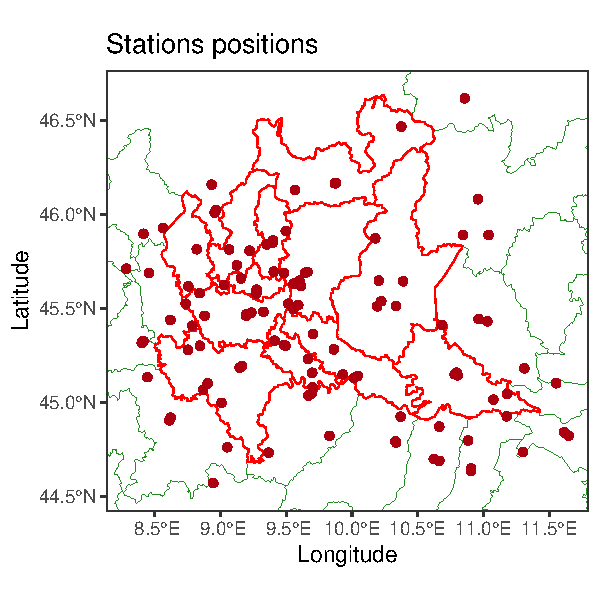
\includegraphics[clip,trim=6px 12px 0px 30px,width=0.45\linewidth]{imgs/stations_map_only_dots.pdf}
%     %     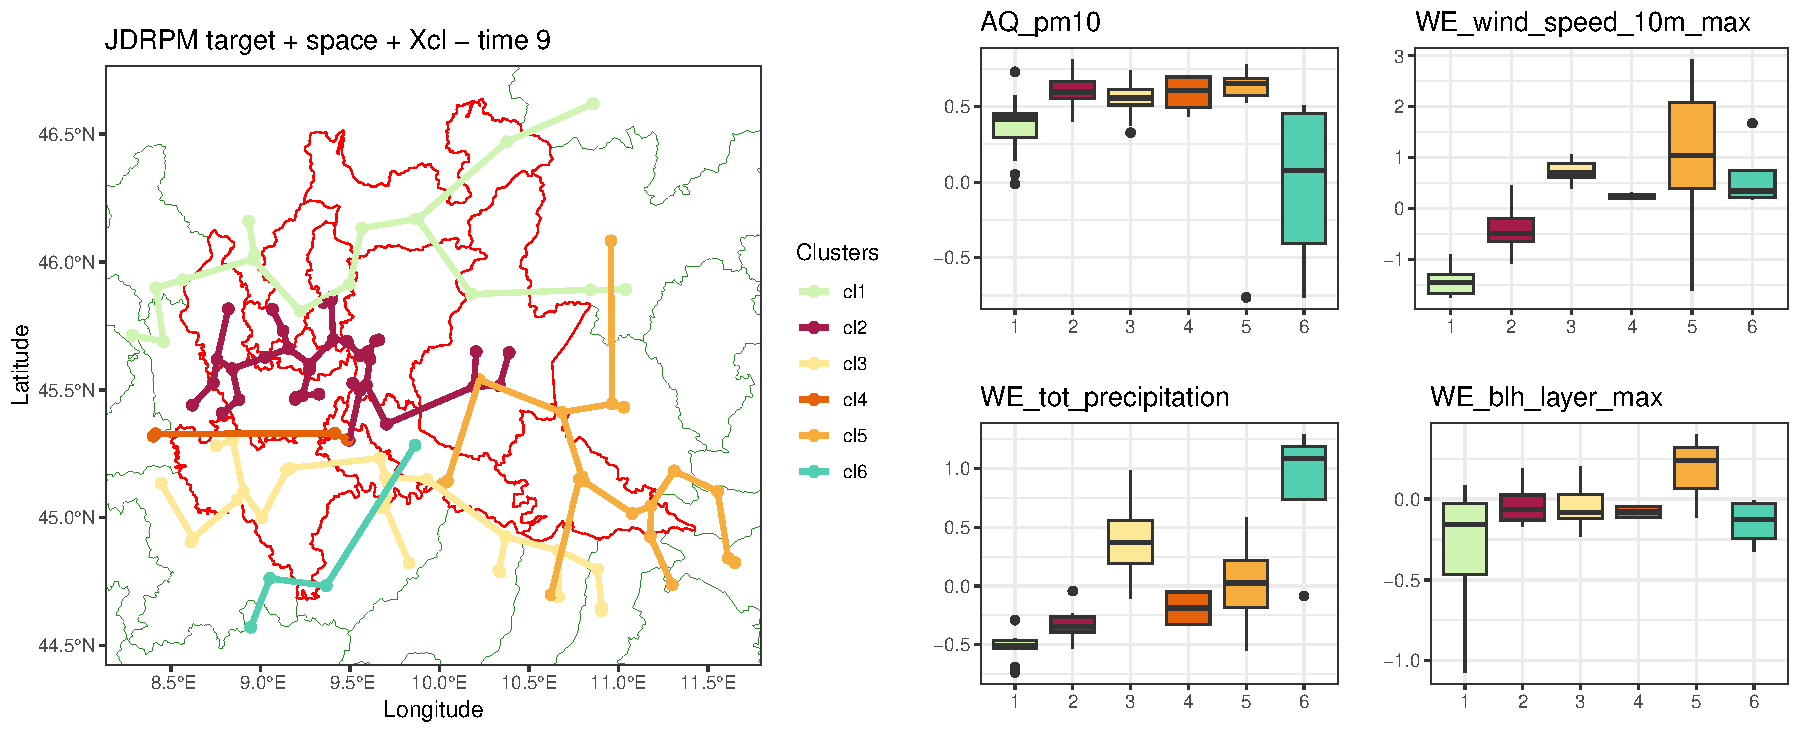
\includegraphics[clip, trim=0px 0px 438px 28px,width=0.53\linewidth]{imgs/JDRPM target + space + Xcl_t09_YLIMS.pdf}
%     % \end{figure}
%     \begin{figure}
%         \centering
%         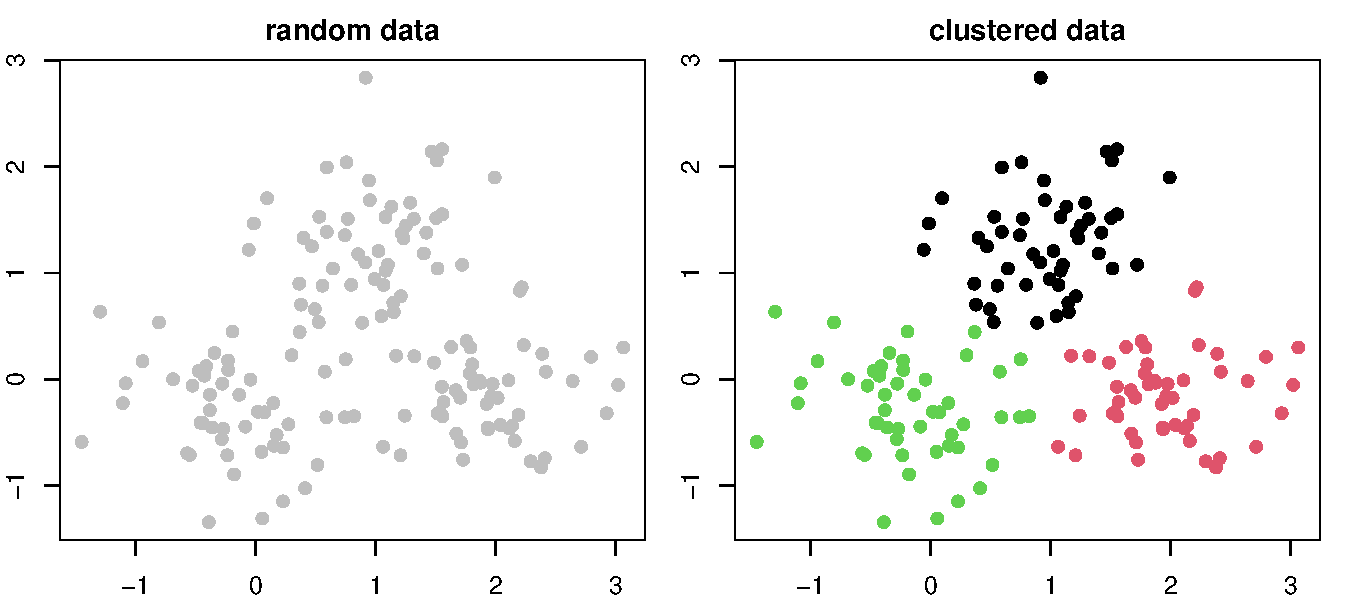
\includegraphics[width=1\linewidth]{imgs/example_clusters_2.pdf}
%         % 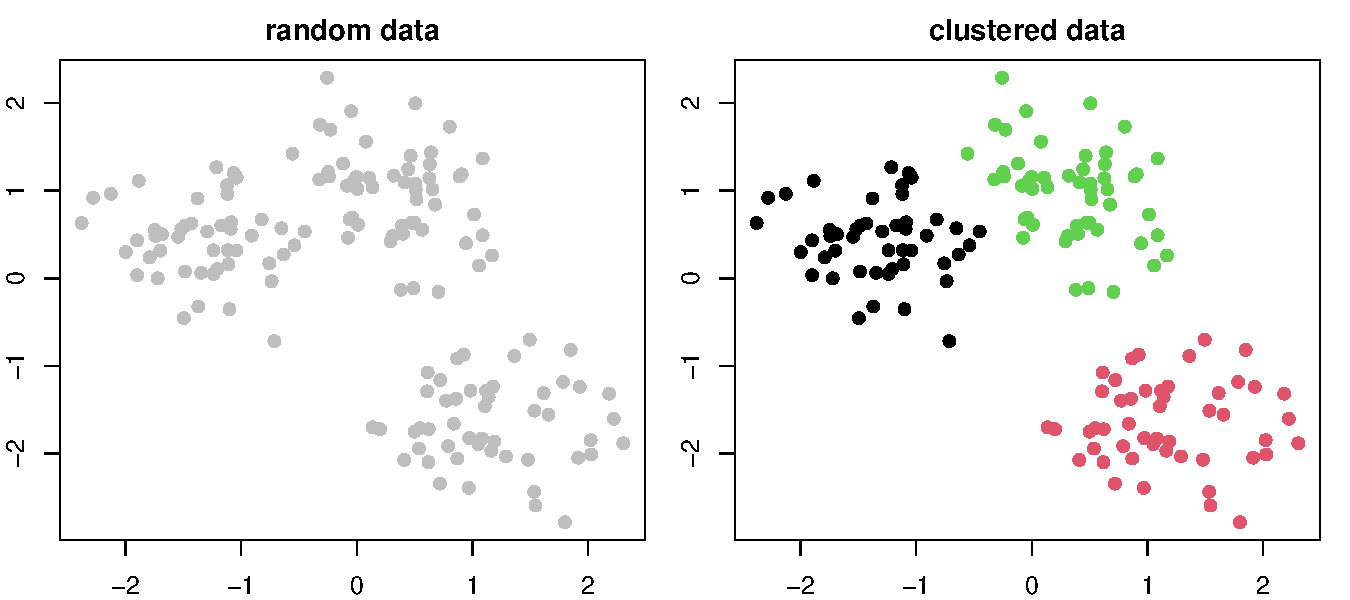
\includegraphics[width=1\linewidth]{imgs/example_clusters.pdf}
%     \end{figure}
% \end{frame}

% \subsection{Methods for clustering}
% \begin{frame}{Algorithmic clustering methods \semoji{smiling-face-with-sunglasses}}
% % Clustering is a fundamental technique of unsupervised learning where a set of data points has to be divided into homogeneous groups of units which exhibit a similar behaviour.\\[5pt]

% Clustering approaches are generally divided into two main categories: algorithmic and model-based methods.

% \vspace{10pt}
% Algorithmic clustering methods address the \balert{clustering problem as an optimization problem} where a certain metric has to be minimised.
% \begin{itemize}
%     \item partition-based methods ($k$-means)
%     \item hierarchical methods (dendrograms)
%     \item density-based methods (DBSCAN)
% \end{itemize}

% However, theese methods are \alert{largely heuristic}, perform well only in relatively \alert{simple scenarios}, and provide \alert{no assessment about clustering uncertainty}, as they lack a solid statistical foundation.

% \end{frame}

% \begin{frame}{Model-based clustering methods \semoji{face-with-raised-eyebrow}}
% In contrast, model-based clustering methods assume a \balert{probabilistic modelling of the data}. This is generally achieved through a \alert{mixture model}, where each mixture component corresponds to a cluster with its specific cluster parameters, so that each observation $i=1,\ldots,n$ is assumed to have arisen from one of the $J$ possible groups which are mixed together in various proportions:
% \begin{equation}
% f(y_i|\vec{\pi},\vec{\theta}^\star_1, \ldots, \vec{\theta}^\star_J)  = \sum_{j=1}^J \pi_j f_j(y_i|\vec{\theta}^\star_j) 
% \label{mixture 1}
% \end{equation}
% where $y_i$ is the data point of the $i$-th observation, $\vec{\pi}$ is the set of weights satisfying $\pi_j \in [0,1]$ for $j=1,\ldots,J$ and $\sum_{j=1}^J \pi_j=1$, $\vec{\theta}_j^\star$ are the cluster-specific parameters, and $f_j(\cdot|\vec{\theta}_j^\star)$ is the density of the $j$-th cluster.
% \end{frame}


% \begin{frame}{Why going Bayesian? \semoji{thinking-face}}
% This approach of a mixture model can be naturally reframed into a \balert{Bayesian context}. But$\ldots$ why one should choose the Bayesian approach?\\[10pt]

% Bayesian models can \alert{incorporate prior information on the parameters}, since each parameter is treated as a random variable with a corresponding prior distribution, allowing in the end to \alert{assess uncertainty in the clusters estimates}.
% \end{frame}


% \begin{frame}{Bayesian mixture models  \semoji{worried-face}}
% We can assume data points to be independent and identically distributed (i.i.d.) from a mixture density, where each mixture component corresponds to a cluster with its cluster-specific parameters, leading \eqref{mixture 1} to be reformulated into:
% \begin{align*}
%     y_i|c_i,\vec{\pi},\vec{\theta}^\star_1, \ldots, \vec{\theta}^\star_J & \simiid f_{c_i}(y_i|\vec{\theta}_{c_i}^\star)\\
%     c_1, \ldots, c_n & \sim \text{Cat}(\pi_1, \ldots, \pi_J)\\
%     \vec{\theta}_1^\star,\ldots,\vec{\theta}_J^\star & \simiid F_0\\
%     \pi_1,\ldots,\pi_J & \sim \text{Dir}(\gamma_1,\ldots,\gamma_J)
%     \numberthis \label{mixture bayesian}
% \end{align*}
% % where the cluster labels $c_1, \ldots, c_n$ are assigned a multinomial distribution with probabilities defined by the vector of weights $\vec{\pi}$, the cluster-specific parameters $\vec{\theta}_j^\star$ are assigned a prior distribution $F_0$, and the weights are assigned a Dirichlet distribution characterized by parameters $\gamma_j$.%which regulate the information incorporated into the model about prior cluster assignments. 
% The clustering labels $c_i$, which identify the component of the mixture each unit is associated to, define the clustering of the units. 
% \end{frame}




% \begin{frame}{Bayesian nonparametric models \semoji{face-with-spiral-eyes}}
% Or, we can transition to a \balert{Bayesian non-parametric context}, where an \alert{infinite mixture model} can be introduced, thus removing the need of a predetermined number $J$ of clusters. In this model, the likelihood of each unit is assigned conditioned to a random parameter, namely
% \begin{align*}
%     y_i|\vec{\theta}_i & \simind f(y_i|\vec{\theta}_i)\\
%     \vec{\theta}_1, \ldots, \vec{\theta}_n|P & \simiid P\\
%     P & \sim \text{discrete RPM} 
%     \numberthis \label{mixture nonparam}
% \end{align*}
% where RPM denotes a random probability measure. The discreteness of $P$ implies the existence of ties among the parameters $\vec{\theta}_1, \ldots, \vec{\theta}_n$ which induce a partition $\rho_n$ identifiable by units that exhibit identical values of the parameter $\vec{\theta}_i$. 
% % More precisely, letting $\vec{\theta}_1^\star, \ldots, \vec{\theta}_K^\star$ be the unique values of $ \vec{\theta}_1, \ldots, \vec{\theta}_n$, the generic $h$-cluster can be defined as $S_h=\{ i \in \{1,\ldots,n\} : \vec{\theta}_i = \vec{\theta}_h^\star \}$. 
% % Therefore, this second class of models specifies the conditional distribution of data points given a realization of the partition of the units, and a prior is assigned to this partition by means of the discreteness of the RPM.
% \end{frame}


% \begin{frame}{Powerful but computational demanding}
% % One of the main tools employed in infinite mixture models is the Dirichlet process (DP) . This allows for modelling the discrete RPM in \eqref{mixture nonparam} as $P|\alpha,P_0 \sim DP(\alpha,P_0)$, where $P_0$ is the base distribution and $\alpha$ is the concentration parameter. The Dirichlet process plays a significant role in Bayesian nonparametrics in general, but particularly in clustering. Its effectiveness is also secured by the various implementation possibilities given by the stick-breaking representation \cite{seth-stick}, the Pólya urn representation \cite{polya-main}, and the Chinese restaurant process (CRP) \cite{aldous-crp}.

% Implementing Bayesian models requires the design of Markov Chain Monte Carlo (MCMC) algorithms, which are often complex and computationally intensive. In MCMC algorithms, complicated or impossible analytical calculations are replaced by simulated approximations derived from a Markov chain that ultimately generates samples from the posterior distribution of the model parameters, allowing inference on the generated quantities.

% % The iterative nature of MCMC, along with the need for a burn-in period, %to allow convergence of the chain to its stationary distribution, 
% % implies that considerable computational resources may be needed.%, particularly for models with high-dimensional parameter spaces or when working with large-scale datasets.
% \end{frame}


% \begin{frame}{Moving to the spatio-temporal context}
    
% The effectiveness of Bayesian model-based approaches, along with their computational demands, becomes particularly pronounced when applied to \alert{spatio-temporal datasets}. Such data, characterized by observations collected over time and across various spatial locations, is inherently complex due to the interplay between spatial and temporal dimensions; a complexity that is further compounded when covariates are also available.\\[10pt]

% However, the Bayesian approach is the most suited approach to address these problems, given the various information levels.
% \end{frame}



% ==============================================
% \section{Description of the model(s)}

% \begin{frame}
% \frametitle{Dependent Random Partition Model}
% \cite{1-drpm}
% \end{frame}

% ==============================================
\section{Implementation and optimizations}
% \frame{\tableofcontents[currentsection, hideothersubsections]}

\subsection{Language choice}
\begin{frame}
\frametitle{Implementation and optimizations}

The MCMC algorithm to compute the posterior samples of our updated model has been implemented in Julia \cite{Julia-cite}, which have several benefits compared to the C choice of \citet{1-drpm}.

\begin{figure}
    \centering
    
\includegraphics[width=0.6\linewidth]{imgs/julia-logo-color-pdfx3.pdf}
\end{figure}
\end{frame}

\begin{frame}{Why Julia?}

\begin{itemize}
    \item Julia combines the ease and expressiveness of high-level languages (e.g. R, python, matlab) with the efficiency and performance characteristics of low-level languages (e.g. C, C++, Fortran)
    \item Julia code can be tested interactively, as with interpreted languages$\ldots$
    \item $\ldots$ but performance is guaranteed through (just-in-time) compilation
    \item Linear algebra computations are optimized through BLAS and LAPACK libraries
    \item There is a vast collection of optimized and complete scientific packages (e.g. \mjline{Statistics}, \mjline{Distributions}, \mjline{MCMCChains}, etc.)
\end{itemize}
\end{frame}

% \begin{frame}{Spoiler alert \semoji{face-with-hand-over-mouth}}
\begin{frame}{Spoiler alert}


% We obtained and improved computational performance, with execution times up to twice as fast  compared to the original C implementation of \cite{1-drpm}, 

% Our implementation in Julia of the generalized DRPM model exhibited improved performances compared to the original C implementation of \cite{1-drpm}, with up to 2x faster execution times.

Using Julia, we obtained \alert{improved computational performance} compared to the original C implementation of \cite{1-drpm}.\\[6pt]
% \begin{block}{}
% Our experiments proved that within the same amount of time in which CDRPM executes a spatially-informed fit, JDRPM can perform a spatially informed fit with up to five covariates in the prior and five covariates in the likelihood.\\[6pt]
% % Our experiments proved that within the same amount of time in which CDRPM executes a spatially-informed fit, JDRPM can perform a spatially informed fit with five covariates in the prior and around five covariates in the likelihood.\\[6pt]
% % since the main performance drop appeared to associated with the increasing of $p_\text{cl}$, rather than of $p_\text{lk}$..\\[6pt]
% \end{block}
% % \begin{figure}
% %     \centering
% %     % \fbox{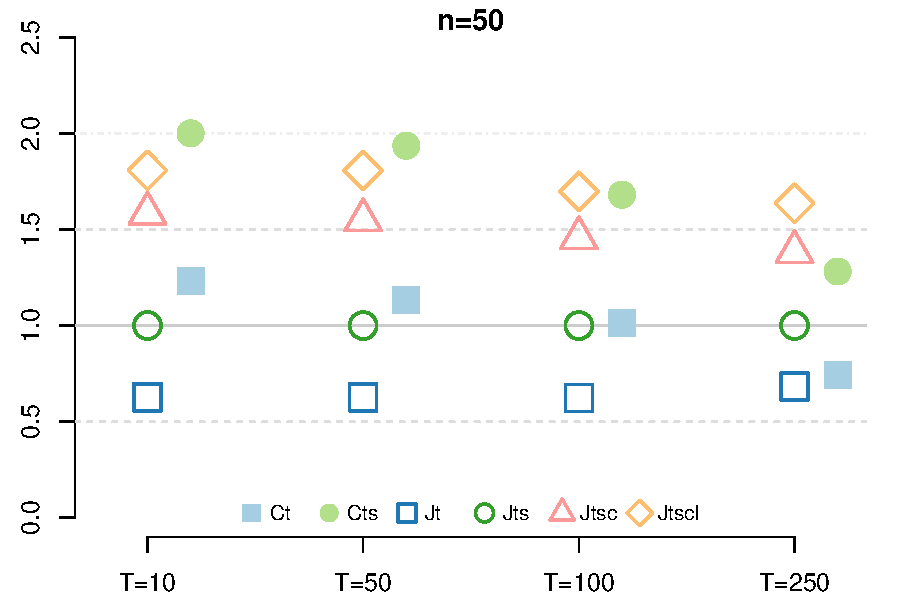
\includegraphics[clip,trim=5px 2px 5px 2px, width=0.58\linewidth]{Testing/Scaling possibilities/summary_performance_n50.pdf}}
% %     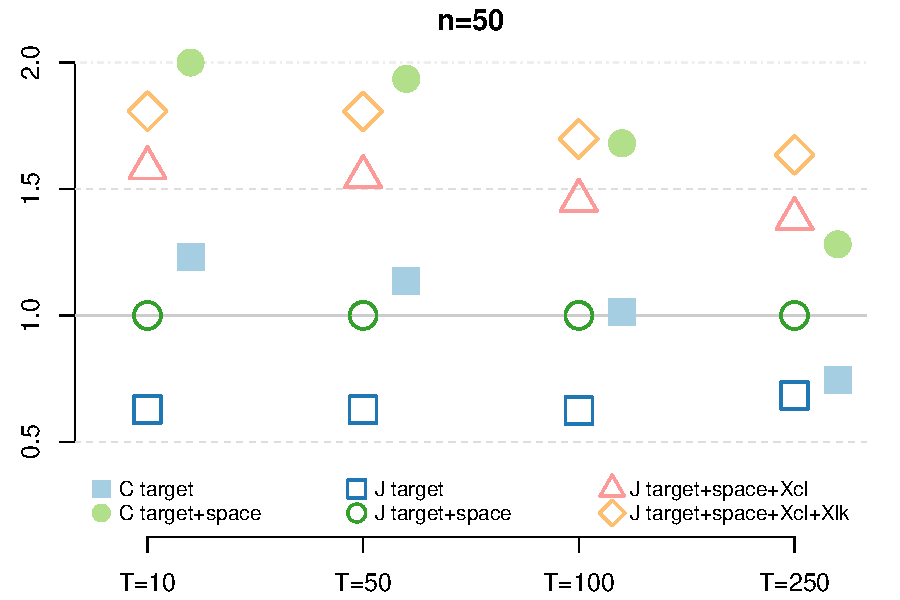
\includegraphics[clip,trim=7px 2px 7px 4px, width=0.58\linewidth]{imgs/summary_performance_n50_legended_bottom.pdf}
% %     % \caption{Enter Caption}
% %     \label{fig:enter-label}
% % \end{figure} 
This performance gain was achieved through several optimizations steps which we now briefly highlight.
\end{frame}

% \begin{frame}{Spoiler alert}

% Using Julia, we obtained \alert{improved computational performance} compared to the original C implementation of \cite{1-drpm}.
% \begin{block}{}
% Our experiments proved that on a standard-sized dataset ($n=50$, $T=50$), these two fits require the same amount of time:
% \begin{itemize}
%     \item CDRPM spatially-informed fit 
%     \item JDPRM spatially-informed fit, with up to five covariates in the prior and five covariates in the likelihood
% \end{itemize}
% \end{block}
% This performance gain was achieved through several optimizations steps which we now briefly highlight.
% \end{frame}


\subsection{Optimizations}

\begin{frame}{General optimizations}

\begin{itemize}
    \item preallocation of all modelling and working variables
    \item ensuring type stability of the code, using the package \mjline{Cthulhu}
\begin{figure}
        \centering
        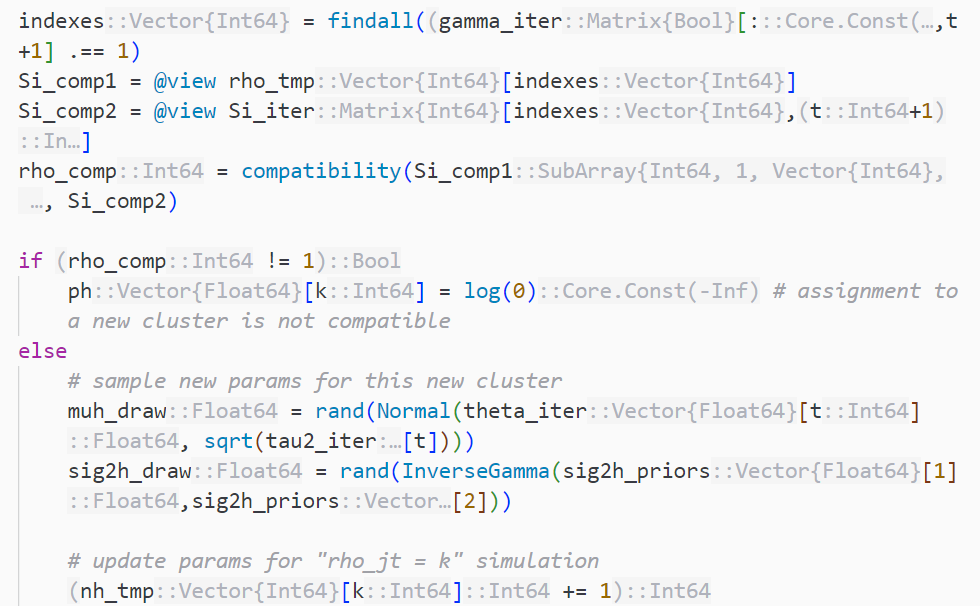
\includegraphics[clip,trim=0px 60px 0px 0px, width=0.94\linewidth]{imgs/ctulhu.png}
        % \caption{Enter Caption}
        \label{fig:enter-label}
    \end{figure}
\end{itemize}
\end{frame}



\begin{frame}[fragile]{General optimizations}

\begin{itemize}
    \item avoiding unnecessary allocations through the \mjline{view} instruction 
\begin{figure}
    \centering
    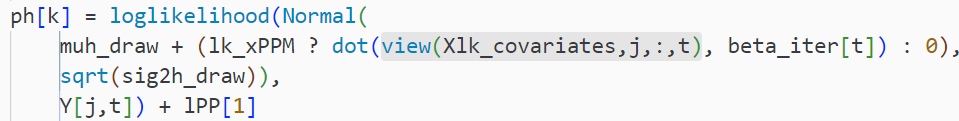
\includegraphics[width=1\linewidth]{zzz/2high.png}
\end{figure}
and through in-place operations
\begin{figure}
    \centering
    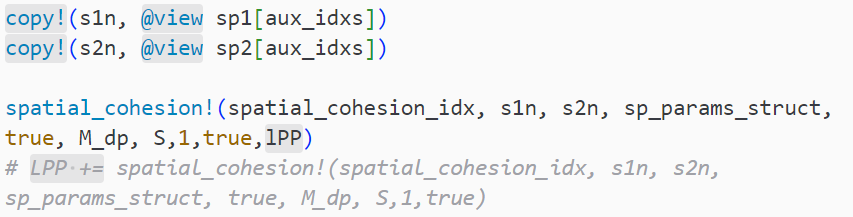
\includegraphics[width=1\linewidth]{zzz/1high.png}
\end{figure}
    % \vspace{-18pt}
    % \item refined the definition of cohesion and similarity functions
\end{itemize}
\end{frame}



\begin{frame}[fragile]{General optimizations}

\begin{itemize}
    \item benchmarking different possible solutions through the package \mjline{BenchmarkTools} %\cite{BenchmarkTools.jl-2016}.
    
    % as in this case, where we are computing the current number of clusters by counting the non-zero entries of the \mjline{nh_tmp} variable\\
    % \vspace{3pt}
\begin{code}
\begin{minted}
[
breaklines,
baselinestretch=1,
autogobble,
% breaksymbolsepleft=2,
fontsize=\footnotesize,
% linenos
mathescape,
tabsize=4,obeytabs
]{julia}
using BenchmarkTools
nh_tmp = rand(100)
@btime nclus_temp = sum($nh_tmp .> 0)
# 168.956 ns (2 allocations: 112 bytes)
@btime nclus_temp = count(x->(x>0), $nh_tmp)
# 11.612 ns (0 allocations: 0 bytes)
\end{minted}
\end{code}
% \vspace{3pt}
    \item refining the definition of cohesion and similarity functions, which are performance-critical since they are called thousands or even millions of times at every fit

\end{itemize}
\end{frame}


\begin{frame}[fragile]{Optimizing spatial cohesions}
% Problem: optimizing 
% \begin{equation*}    
% C_3(S_{h},\vec{s}_{h}^\star) = M \cdot \Gamma(|S_h|) \cdot \int \prod_{i \in S_h} q(\vec{s}_i|\vec{\csi}_h) q(\vec{\csi}_h) \, d\vec{\csi}_h
% \end{equation*}
% and
% \begin{equation*}
% C_4(S_{h},\vec{s}_{h}^\star) = M \cdot \Gamma(|S_h|) \cdot \int \prod_{i \in S_h} q(\vec{s}_i|\vec{\csi}_h) q(\vec{\csi}_h|\vec{s}_h^\star) \, d\vec{\csi}_h
% \end{equation*}

Problem: optimizing cohesions $C_3$ and $C_4$.

Solution v1: naive vector implementation.

\begin{code}
% \caption[Three versions of cohesion 3 and 4 implementation]{Snippets of Julia code for the three implementation solutions of the spatial cohesions 3 and 4. The first is the naive vector implementation, the second is its scalar conversion, and the third is the static vector solution.}
 % # this is a standard vector
% # all the following matrices and vector will be standard structures
\label{list: cohes3}
\begin{minted}
[
breaklines,
baselinestretch=1,
autogobble,
% breaksymbolsepleft=2,
fontsize=\footnotesize,
% linenos
mathescape,escapeinside=||,
tabsize=4,obeytabs
]{julia}
sbar = [mean(s1), mean(s2)]
vtmp = sbar - mu_0 
Mtmp = vtmp * vtmp'
Psi_n = Psi + S + (k0*sdim) / (k0+sdim) * Mtmp
|$\vdots$|
\end{minted}
\end{code}
\end{frame}

\begin{frame}[fragile]{Optimizing spatial cohesions}

Problem: optimizing cohesions $C_3$ and $C_4$.

Solution v2: implementation using only scalar variables.

\begin{code}
% \caption[Three versions of cohesion 3 and 4 implementation]{Snippets of Julia code for the three implementation solutions of the spatial cohesions 3 and 4. The first is the naive vector implementation, the second is its scalar conversion, and the third is the static vector solution.}
\label{list: cohes3}
\begin{minted}
[
breaklines,
baselinestretch=1,
autogobble,
% breaksymbolsepleft=2,
fontsize=\footnotesize,
% linenos
mathescape,escapeinside=||,
tabsize=4,obeytabs
]{julia}
sbar1 = mean(s1)
sbar2 = mean(s2)
vtmp_1 = sbar1 - mu_0[1]
vtmp_2 = sbar2 - mu_0[2]
Mtmp_1 = vtmp_1^2
Mtmp_2 = vtmp_1 * vtmp_2
Mtmp_3 = copy(Mtmp_2)
Mtmp_4 = vtmp_2^2
aux1 = k0 * sdim; aux2 = k0 + sdim
Psi_n_1 = Psi[1] + S1 + aux1 / (aux2) * Mtmp_1
Psi_n_2 = Psi[2] + S2 + aux1 / (aux2) * Mtmp_2
Psi_n_3 = Psi[3] + S3 + aux1 / (aux2) * Mtmp_3
Psi_n_4 = Psi[4] + S4 + aux1 / (aux2) * Mtmp_4
|$\vdots$|
\end{minted}
\end{code}
\end{frame}


\begin{frame}[fragile]{Optimizing spatial cohesions}

Problem: optimizing cohesions $C_3$ and $C_4$.

Solution: implementation using static vectors and matrices.

\begin{code}
% \caption[Three versions of cohesion 3 and 4 implementation]{Snippets of Julia code for the three implementation solutions of the spatial cohesions 3 and 4. The first is the naive vector implementation, the second is its scalar conversion, and the third is the static vector solution.}
% # this is a statically-sized vector
% # all the following matrices and vector will be statically-sized
\label{list: cohes3}
\begin{minted}
[
breaklines,
baselinestretch=1,
autogobble,
% breaksymbolsepleft=2,
fontsize=\footnotesize,
% linenos
mathescape, escapeinside=||,
tabsize=4,obeytabs
]{julia}
using |\fbox{StaticArrays}|
sbar1 = mean(s1); sbar2 = mean(s2)
sbar = |\fbox{SVector}|((sbar1, sbar2))
vtmp = sbar .- mu_0 
Mtmp = vtmp * vtmp'
aux1 = k0 * sdim; aux2 = k0 + sdim
Psi_n = Psi .+ S .+ aux1 / (aux2) .* Mtmp
|$\vdots$|
\end{minted}
\end{code}
\end{frame}


\begin{frame}{Optimizing spatial cohesions}
    \begin{figure}[!ht]
\centering
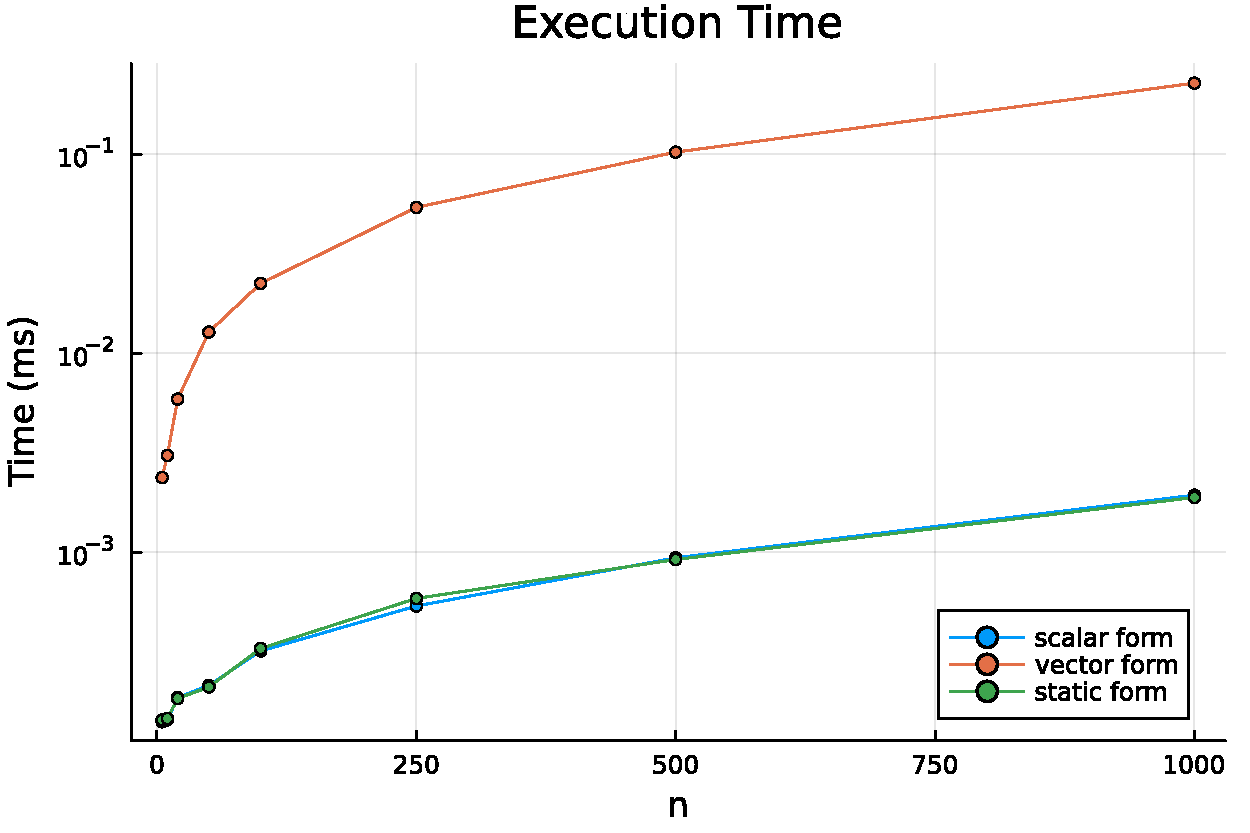
\includegraphics[width=0.9\linewidth]{Plots/execution_time.pdf}
% \caption[Performance comparison of cohesions 3 and 4 implementations]{Performance comparison among the three versions of the cohesion 4 function. Similar results stand for cohesion 3. Panels (a) and (b) are constant at zero for both the scalar and static cases.}
\label{fig: cohesion3 comparison}
\end{figure}
\end{frame}

\begin{frame}{Optimizing spatial cohesions}
    \begin{figure}[!ht]
\centering
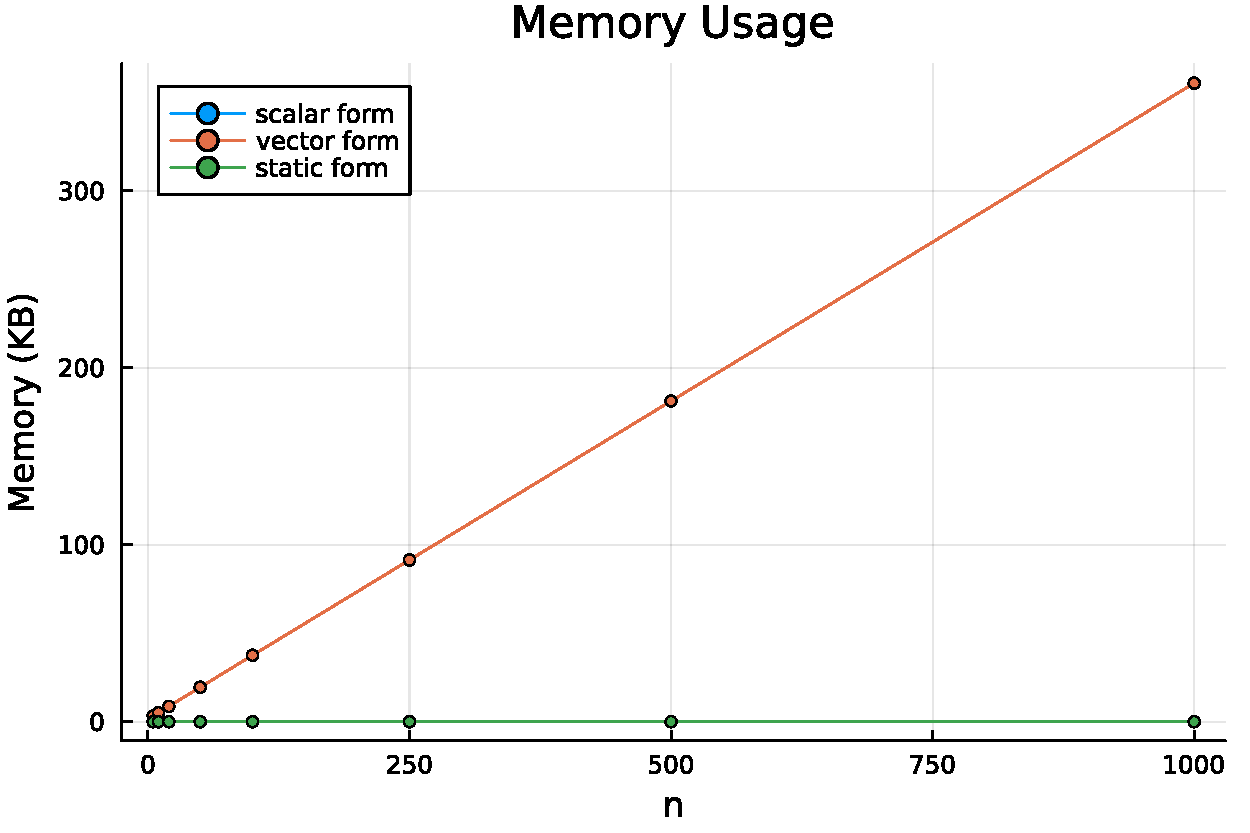
\includegraphics[width=0.9\linewidth]{Plots/memory_usage.pdf}
% \caption[Performance comparison of cohesions 3 and 4 implementations]{Performance comparison among the three versions of the cohesion 4 function. Similar results stand for cohesion 3. Panels (a) and (b) are constant at zero for both the scalar and static cases.}
\label{fig: cohesion3 comparison}
\end{figure}
\end{frame}


\begin{frame}[fragile]{Optimizing covariates similarities}

Problem: optimizing similarity $g_4$.

Solution: employing some optimizing macros on the inner loop.

    \begin{code}
% \caption[Similarity 4 implementation with all optimizing annotations]{Similarity 4 function implementation, with all optimizing annotations. The performance analysis will just focus on that inside loop.}
\label{list: sim4}
\begin{minted}
[breaklines,
baselinestretch=1,
autogobble,
% breaksymbolsepleft=2,
fontsize=\footnotesize,
% linenos
mathescape, escapeinside=||,
tabsize=4,obeytabs
]{julia}
function similarity4(X_jt::AbstractVector{<:Real}, mu_c::Real, lambda_c::Real, a_c::Real, b_c::Real, lg::Bool)
	n = length(X_jt); nm = n/2
	xbar = mean(X_jt)
	aux2 = 0.
	|\fbox{@inbounds @simd}| for i in eachindex(X_jt)
		aux2 += X_jt[i]^2
	end
	aux1 = b_c + 0.5 * (aux2 - (n*xbar + lambda_c*mu_c)^2/(n+lambda_c) + lambda_c*mu_c^2 )
	out = -nm*log2pi + 0.5*log(lambda_c/(lambda_c+n)) + lgamma(a_c+nm) - lgamma(a_c) + a_c*log(b_c) + (-a_c-nm)*log(aux1)
	return lg ? out : exp(out)
end
\end{minted}
%	|\fbox{@inbounds @fastmath @simd}| for i in eachindex(X_jt)
\end{code}
\end{frame}

% \begin{frame}[fragile]{Optimizing covariates similarities}

% \begin{code}
% \begin{minted}
% [breaklines,
% baselinestretch=1,autogobble,
% fontsize=\small,
% mathescape,escapeinside=||,tabsize=4,obeytabs
% ]{julia}
% |\fbox{@inbounds}| @fastmath @simd for i in eachindex(X_jt)
% 	aux2 += X_jt[i]^2
% end
% \end{minted}
% \end{code}
% \vspace{6pt}
% \mjline{@inbounds} eliminates array bounds checking within expressions, thus saving execution time. This annotation is safe to use as long as we can guarantee that the code will not access elements outside the array bounds; otherwise undefined behaviour may occur.
% \end{frame}

% \begin{frame}[fragile]{Optimizing covariates similarities}

% \begin{code}
% \begin{minted}
% [breaklines,
% baselinestretch=1,autogobble,
% fontsize=\small,
% mathescape,escapeinside=||,tabsize=4,obeytabs
% ]{julia}
% @inbounds |\fbox{@fastmath}| @simd for i in eachindex(X_jt)
% 	aux2 += X_jt[i]^2
% end
% \end{minted}
% \end{code}
% \vspace{6pt}
% \mjline{@fastmath} executes a modified version of the expression that may invoke functions violating strict IEEE semantics. For instance, using this macro could result in $(a+b)+c \neq a+(b+c)$, but only in highly pathological cases. \phantom{y}
% \end{frame}

% \begin{frame}[fragile]{Optimizing covariates similarities}

% \begin{code}
% \begin{minted}
% [breaklines,
% baselinestretch=1,autogobble,
% fontsize=\small,
% mathescape,escapeinside=||,tabsize=4,obeytabs
% ]{julia}
% @inbounds @fastmath |\fbox{@simd}| for i in eachindex(X_jt)
% 	aux2 += X_jt[i]^2
% end
% \end{minted}
% \end{code}
% \vspace{6pt}
% \mjline{@simd} (Single Instruction Multiple Data) is a technique akin to parallelism, but rather than distributing the computational load across multiple processors, we let the CPU execute the same instruction on multiple data chunks simultaneously using vector registers.
% \end{frame}

% \begin{frame}{Optimizing covariates similarities}
% \begin{itemize}
%     \item \mjline{@inbounds} eliminates array bounds checking within expressions, thus saving execution time. This annotation is safe to use as long as we can guarantee that the code will not access elements outside the array bounds; otherwise undefined behaviour may occur. 
%     % In our case, the loop structure is simple and safe, so this assumption holds true.
%     \item \mjline{@fastmath} executes a modified version of the expression that may invoke functions violating strict IEEE semantics. For instance, using this macro could result in $(a+b)+c \neq a+(b+c)$, but only in highly pathological cases. 
%     % Again, this is not an issue for our loop, which computes $\sum X_i^2$, as there is no intrinsic "correct order" for performing this operation.
%     \item \mjline{@simd} (Single Instruction Multiple Data) is a technique akin to parallelism, but rather than distributing the computational load across multiple processors, we let the CPU execute the same instruction on multiple data chunks simultaneously.% using vector registers.
%     % As a result, this approach accelerates computation by eliminating the need to process each element of the vector individually.
% \end{itemize}
% \end{frame}


\begin{frame}{Optimizing covariates similarities}

    \begin{figure}[!ht]
    \centering
    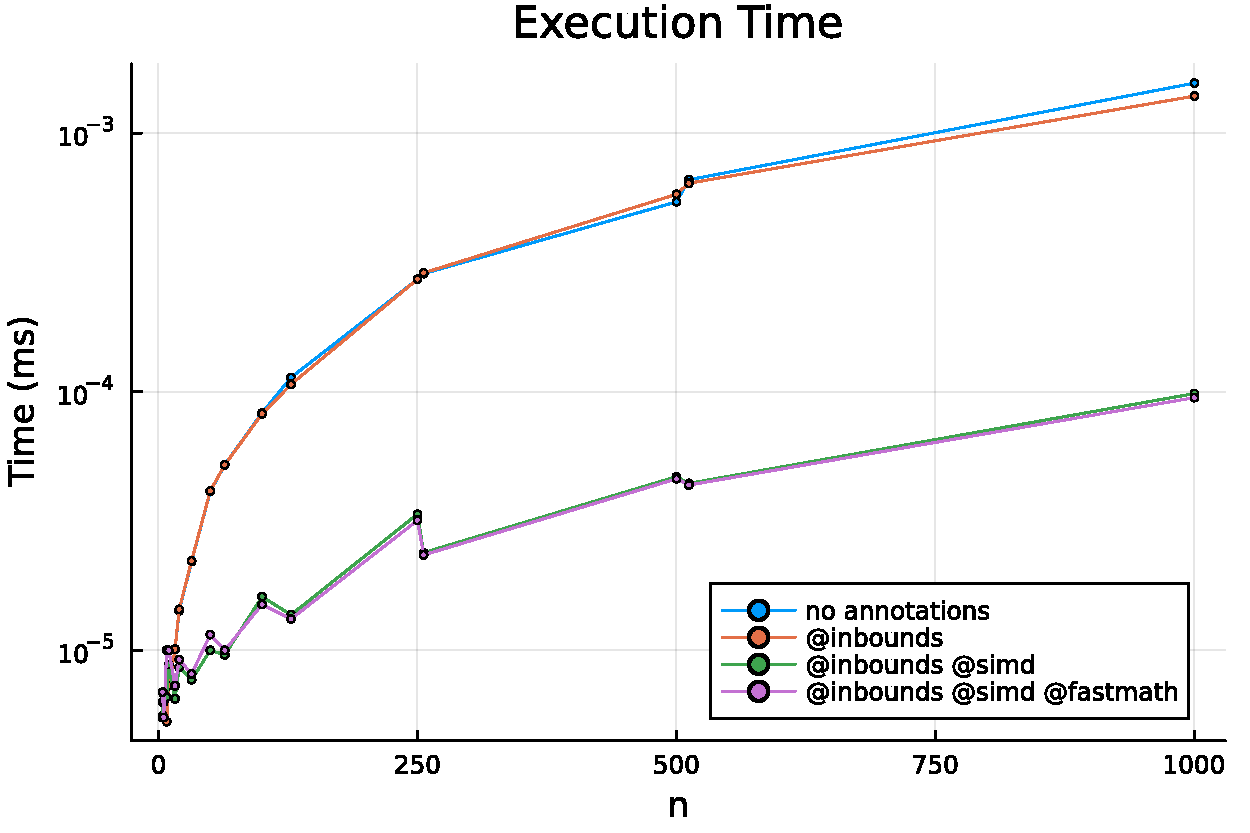
\includegraphics[width=0.9\linewidth]{Plots/execution_time_tests_sims_pow2.pdf}
    % \caption[Performance comparison of similarity 4 annotations]{Performance comparison of the different loop annotations in the similarity 4 implementation.}
    \label{fig: exec time sim}
\end{figure}

\end{frame}



% ==============================================
\section{Analysis of the models}
% \frame{\tableofcontents[currentsection, hideothersubsections]}


% \begin{frame}{Contents}
% \begin{enumerate}
%     \item Introduction
%     \item Description of the model(s)
%     \item Implementation and optimizations\\[10pt]
%     \item \balert{Analysis of the models}\\
%     Experiments conducted on CDRPM and JDRPM\\[10pt]
%     \item Conclusion
% \end{enumerate}\end{frame}

\subsection{Comparing the two algorithms}
% \frame{\tableofcontents[currentsection, currentsubsection,subsectionstyle=show/shaded/hide, hideothersubsections]}

\begin{frame}{Comparing the two algorithms}
% Our model, along with its corresponding MCMC algorithm, represents a generalization of the original DRPM and its associated algorithm.

Our model represents a generalization of the original DRPM and its associated MCMC algorithm. 
% In this sense, our updates serve as extensions to the original model; 
Therefore, under identical datasets, hyperparameters, and MCMC configurations, both models are expected to perform similarly and produce comparable clusters estimates.\\[6pt]
To evaluate the numerical performance of both algorithms, we will analyse posterior samples and clusters estimates in two scenarios: 
\begin{enumerate}
    \item using a synthetic dataset that includes only the response variable
    \item employing a real-world spatio-temporal dataset, derived from the AgrImOnIA project \cite{agrimonia}
\end{enumerate}

% The latter dataset also provides covariates, whose effects will be examined later in a dedicated section.
\end{frame}

\begin{frame}{Simulated data scenario}

For the first comparison we generated a dataset consisting of $n=10$ units and $T=12$ time instants. 
% The data generating function was the same employed in \cite{1-drpm} for their analyses, and it allows for the creation of data points with temporal dependence. %which could be adjusted through specific parameters. 
Both algorithms were executed collecting 2000 iterates from a total of 50000 iterations, by discarding the first 40000 as burnin and then thinning by 5.
\begin{figure}[!p]
    \centering
    \includegraphics[width=0.8\linewidth]{Testing//Assessing correctness//no space/test_1_generated_data.pdf}
    % 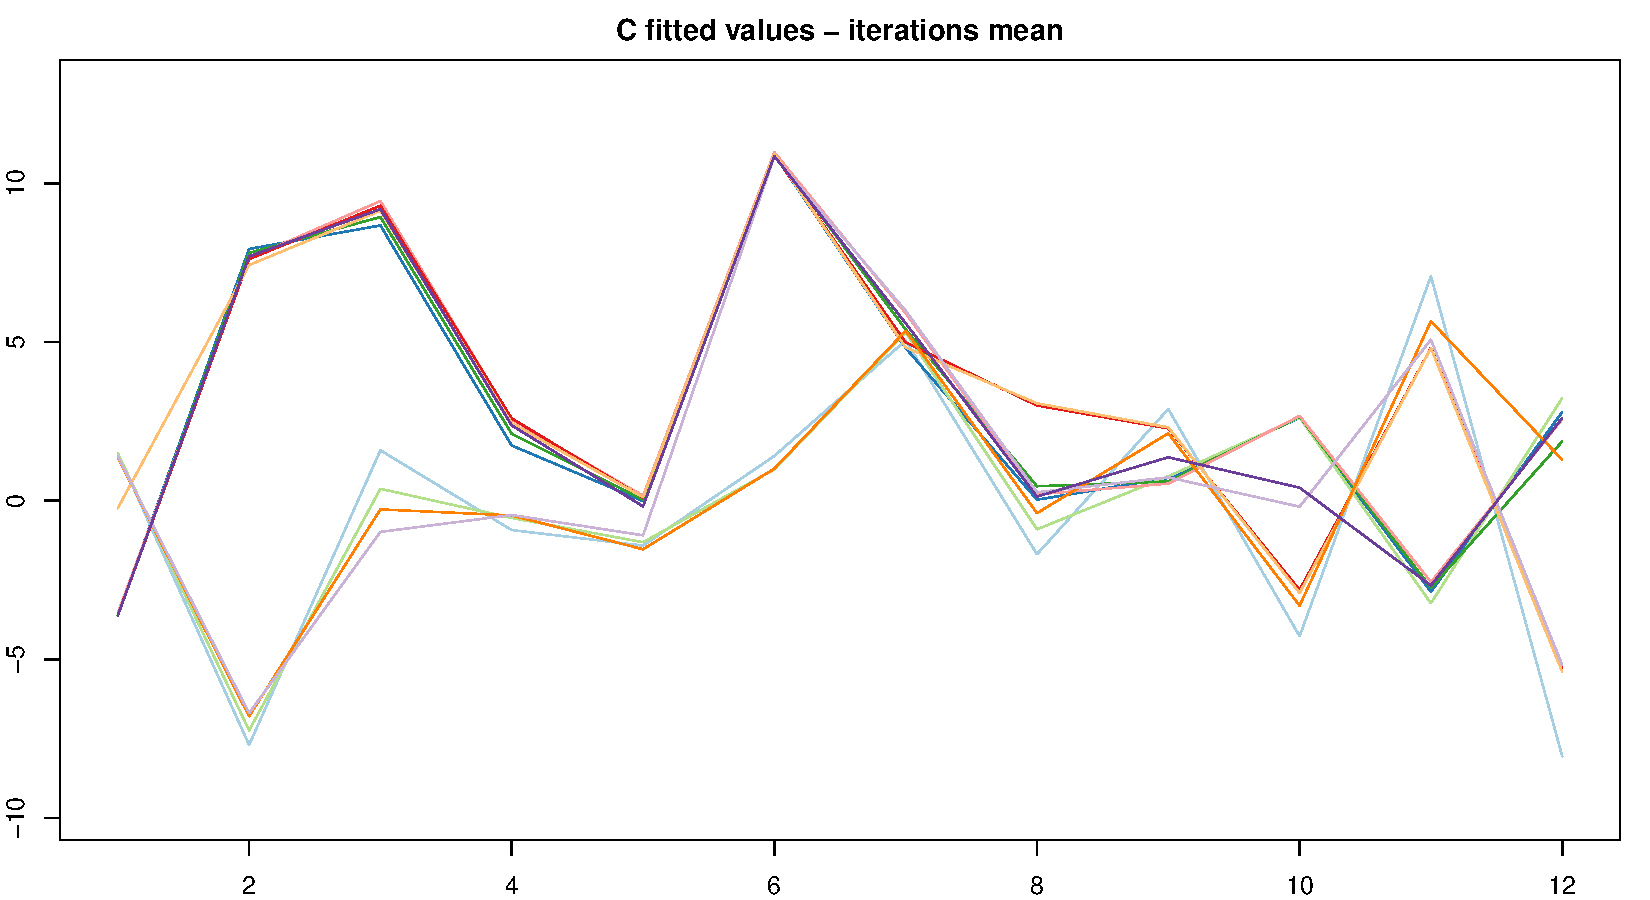
\includegraphics[width=0.97\linewidth]{Testing//Assessing correctness//no space/C_mean_prediction.pdf}
    % 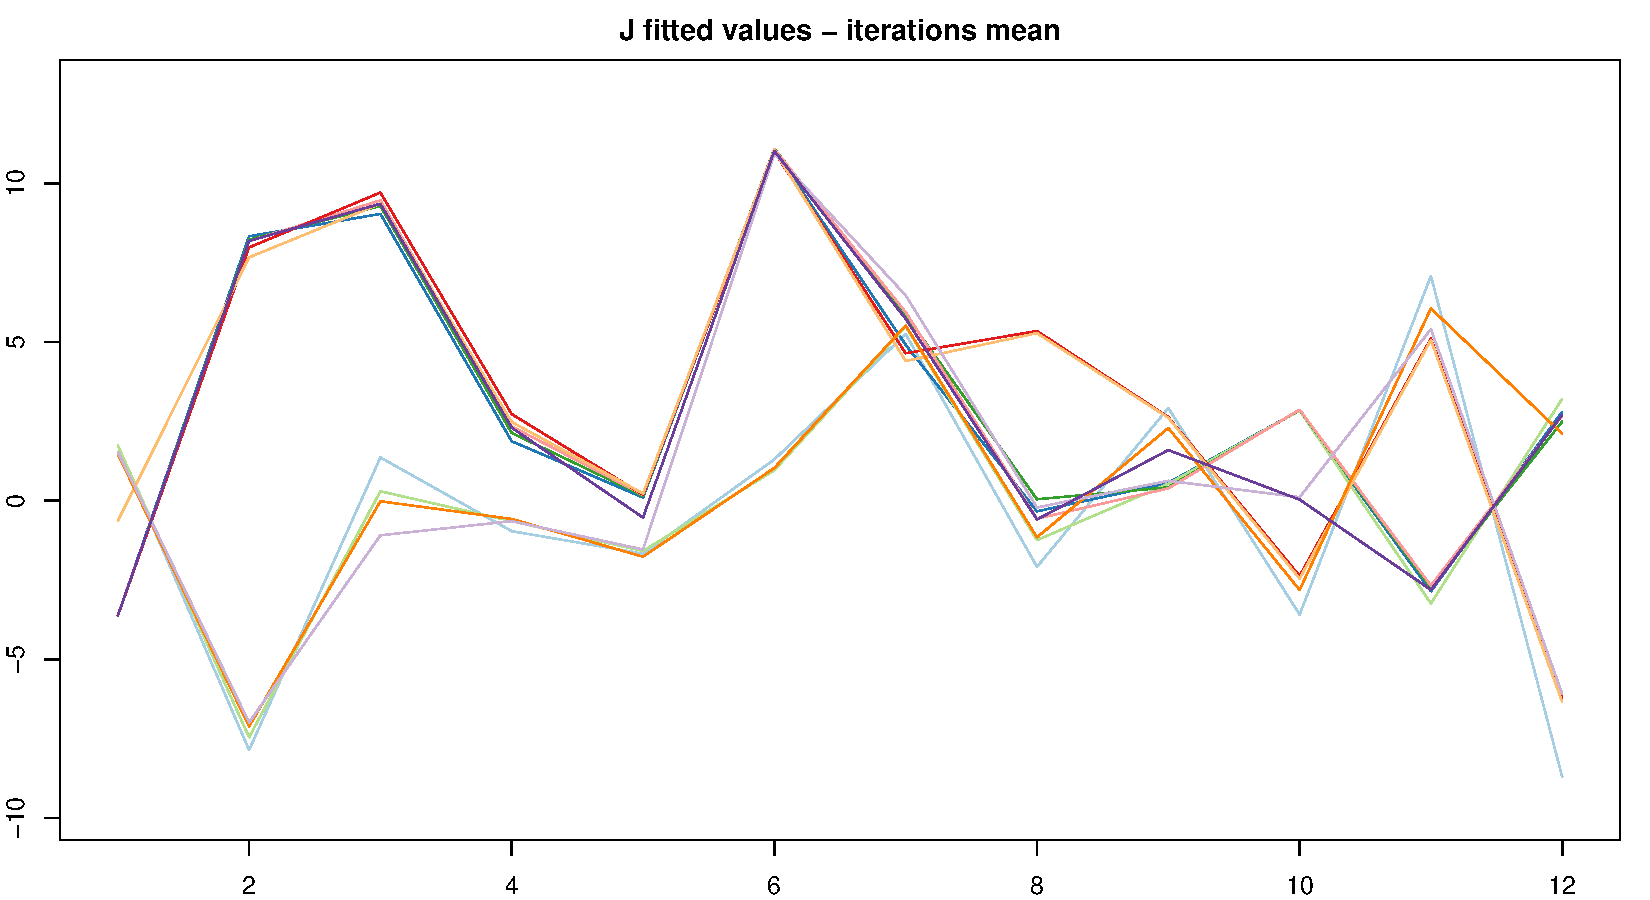
\includegraphics[width=0.97\linewidth]{Testing//Assessing correctness//no space/J_mean_prediction.pdf}
    % \caption[Fitted values of CDRPM and JDRPM, simulated data scenario]{Fitted values of CDRPM (middle) and JDRPM (bottom) fits, in the simulated data scenario, alongside the generated target values (top).}
    \label{fig: fitted and target values no space}
\end{figure}
\end{frame}

\begin{frame}{Simulated data scenario}

    \begin{table}[!htb]
    % \caption[Accuracy metrics of CDRPM and JDRPM fits, target values only]{Summary of the comparison between the two fits on target values only. The MSE columns refer to the accuracy between the fitted values generated by the models (estimated by taking the mean and the median of the returned 1000 iterates) and the true values of the target variable. Higher LPML and lower WAIC indicate a better fit.}
    % \caption[Comparison of CDRPM and JDRPM, simulated data scenario]{Comparison between CDRPM and JDRPM fits and their associated algorithms, in the simulated data scenario.}
    \centering
    % \begin{tabular}{cccccc}
    \resizebox{0.7\linewidth}{!}{%
    \begin{tabular}{cccc}
    \toprule
       % & MSE mean &  MSE median & LPML & WAIC & exec. time  \\
       % \midrule
       %  CDRPM &  1.6731  & 1.5861  & -249.61 & 469.69 & 4.8s\\
       %  JDRPM & \textbf{1.2628}  & \textbf{1.2181}  & \textbf{-227.83} &  \textbf{415.03}  &  \textbf{2.5s} \\
       %  \bottomrule
          & MSE mean &  MSE median & execution time  \\
       \midrule
        CDRPM &   1.6221  &  1.5823  & 19s\\
        JDRPM & \textbf{1.2634}  & \textbf{1.2034}  &   \textbf{13s} \\
        \bottomrule
    \end{tabular}
    \label{tab: fits metrics no space}
    }
\end{table}
\begin{figure}[!htb]
    \centering
    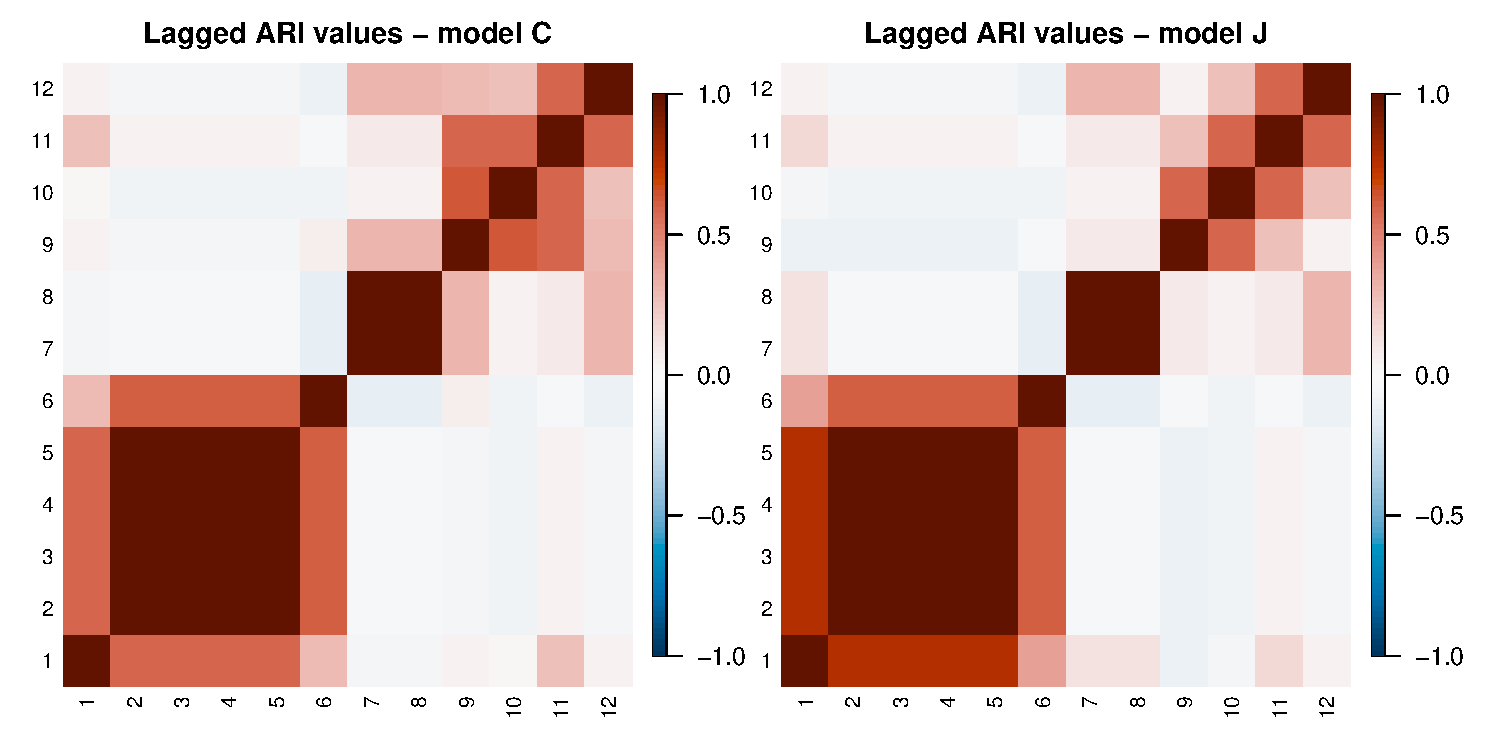
\includegraphics[width=0.9\linewidth]{Testing/Assessing correctness/no space/ari.pdf}
    % \caption[Lagged ARI values of CDRPM and JDRPM, simulated data scenario]{Lagged ARI values of CDRPM and JDRPM fits, in the simulated data scenario.}
    \label{fig:ari no space}
\end{figure}
\end{frame}

\begin{frame}{Simulated data scenario}

 Computing the adjusted Rand index $\ari(\rho_{\text{JDRPM}}(t),\rho_{\text{CDRPM}}(t))$ for all time instants $t=1,\ldots,12$, we obtained a \alert{mean of 0.95} and a \alert{median of 1}.
    \begin{figure}[!htb]
    \centering
    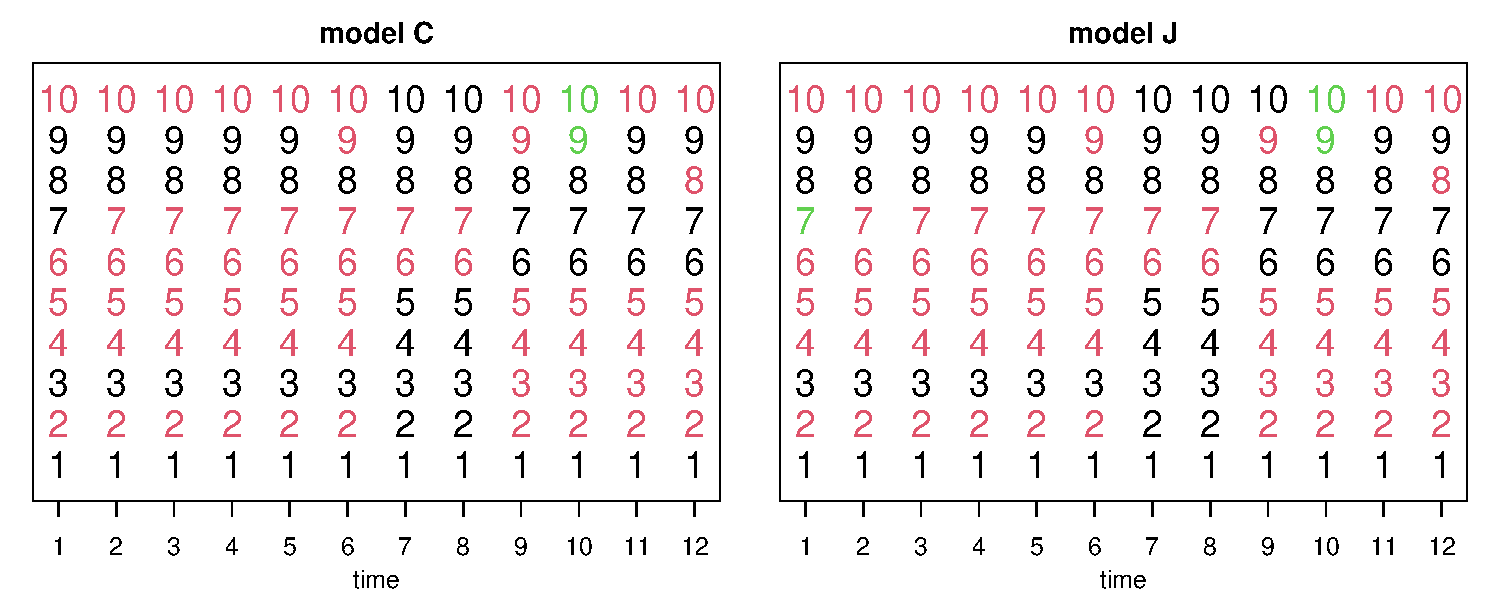
\includegraphics[width=1\linewidth]{Testing/Assessing correctness/no space/partizioni_nums.pdf}
    % \caption[Clusters estimates of CDRPM and JDRPM, simulated data scenario]{Clusters estimates produced by CDRPM and JDRPM fits, in the simulated data scenario. Time instants are annotated on the $x$ axis, units are indicated vertically by their number, and colors represent the cluster label.}
    % \caption{$\ari(\rho_{\text{JDRPM}}(t),\rho_{\text{CDRPM}}(t))$, computed over all time instants $t=1,\ldots,T$, has a mean of 0.95 and a median of 1.}
    \label{fig:partizioni no space}
\end{figure}
\end{frame}
% \begin{frame}{Simulated data scenario}

% \begin{figure}[!htb]
%     \centering
%     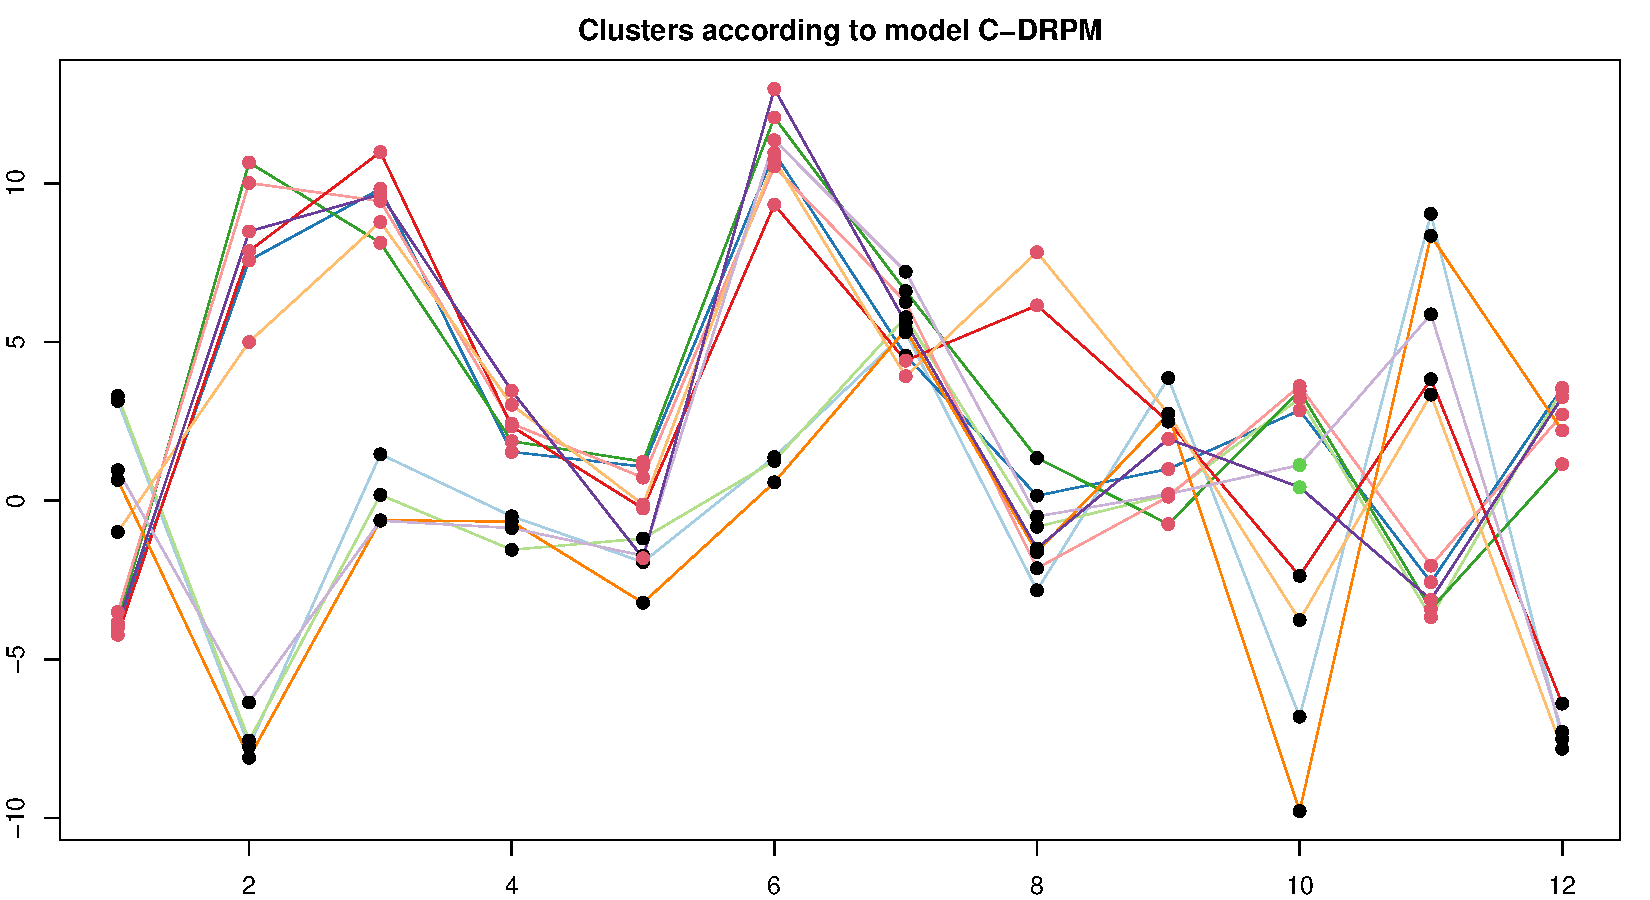
\includegraphics[width=1\linewidth]{Testing/Assessing correctness/no space/clusters_C.pdf}
%     % 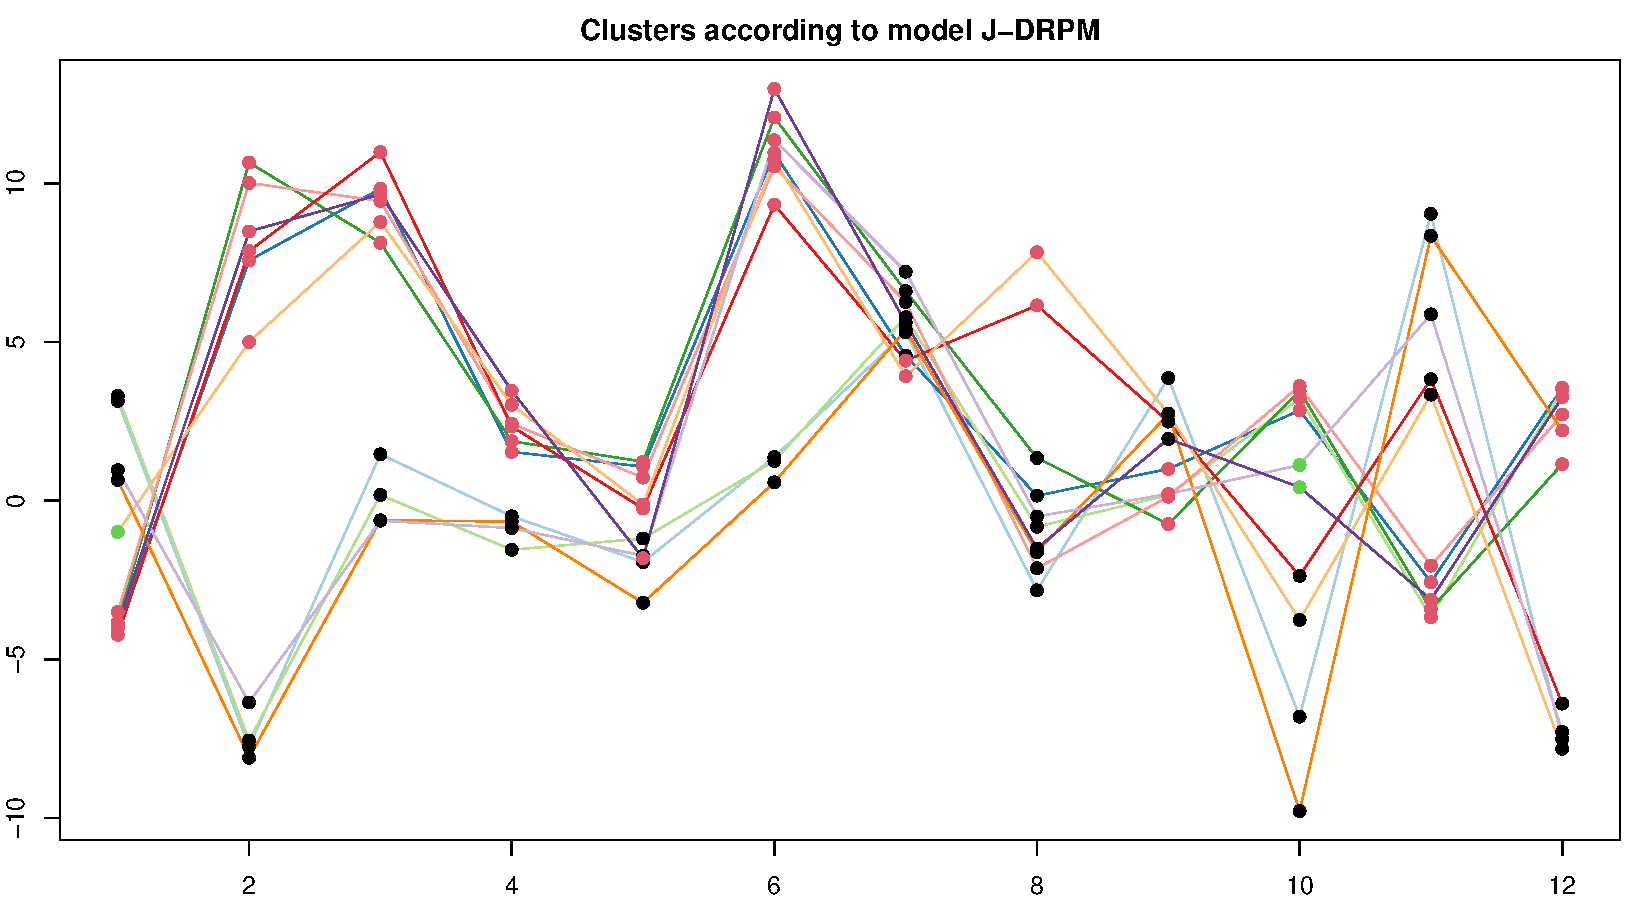
\includegraphics[width=1\linewidth]{Testing/Assessing correctness/no space/clusters_J.pdf}
%     % \caption[Visual representation of the clusters estimates of CDRPM and JDRPM, simulated data scenario]{Visual representation of the clusters estimates produced by CDRPM and JDRPM fits, in the simulated data scenario. Cluster labels are represented as colored dots overlaid to the trend of the target variable.}
%     \label{fig:clusters no space}
% \end{figure}
% \end{frame}
% \begin{frame}{Simulated data scenario}

% \begin{figure}[!htb]
%     \centering
%     % 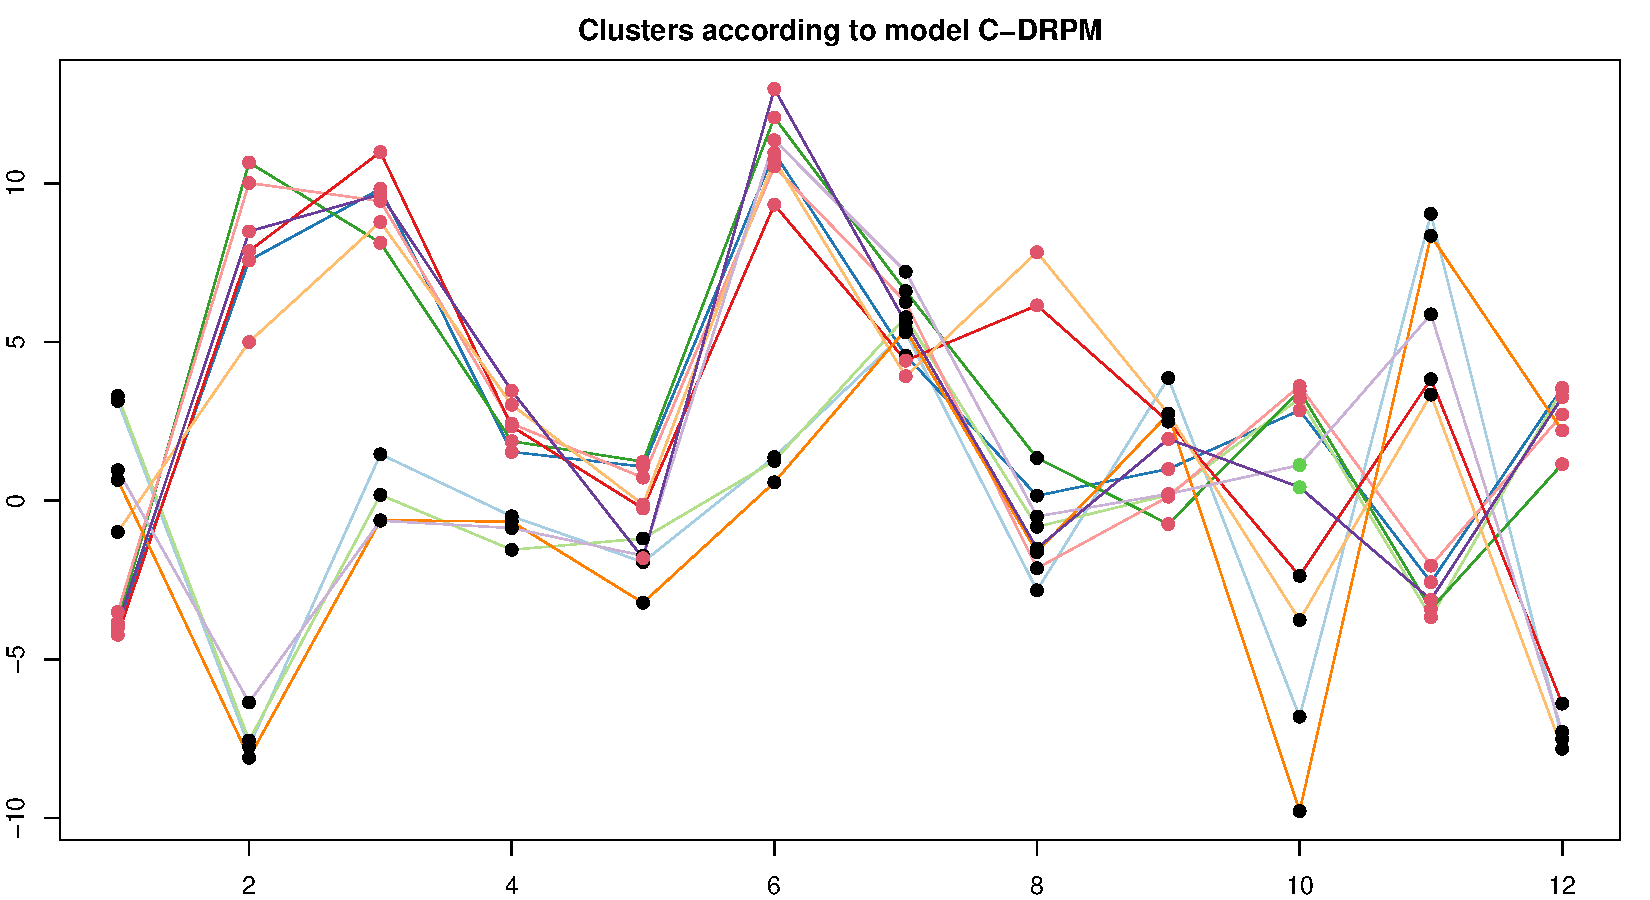
\includegraphics[width=1\linewidth]{Testing/Assessing correctness/no space/clusters_C.pdf}
%     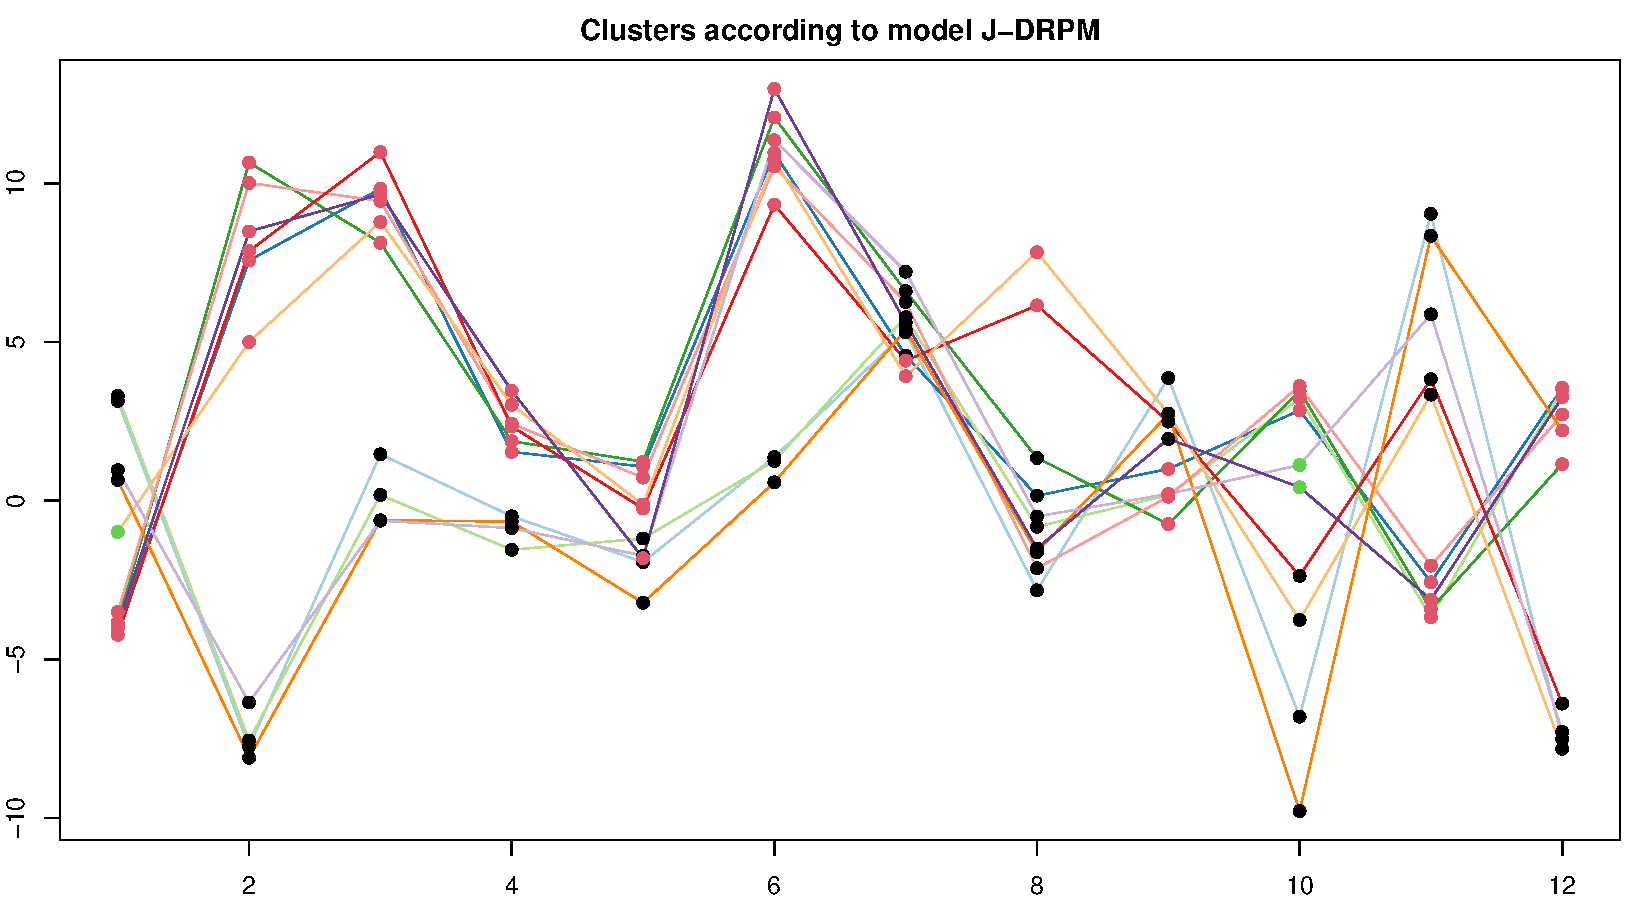
\includegraphics[width=1\linewidth]{Testing/Assessing correctness/no space/clusters_J.pdf}
%     % \caption[Visual representation of the clusters estimates of CDRPM and JDRPM, simulated data scenario]{Visual representation of the clusters estimates produced by CDRPM and JDRPM fits, in the simulated data scenario. Cluster labels are represented as colored dots overlaid to the trend of the target variable.}
%     \label{fig:clusters no space}
% \end{figure}
% \end{frame}

\begin{frame}{Real-world scenario}

For the second comparison, we employed a dataset comprising weekly averages of $\pmten$ values from the year 2018, measured by $n=105$ units for $T=12$ time instants. We collected 4000 iterates from 110000 total iterations, by discarding the first 90000 as burnin and then thinning by 5.
\begin{figure}[!ht]
    \centering
    % 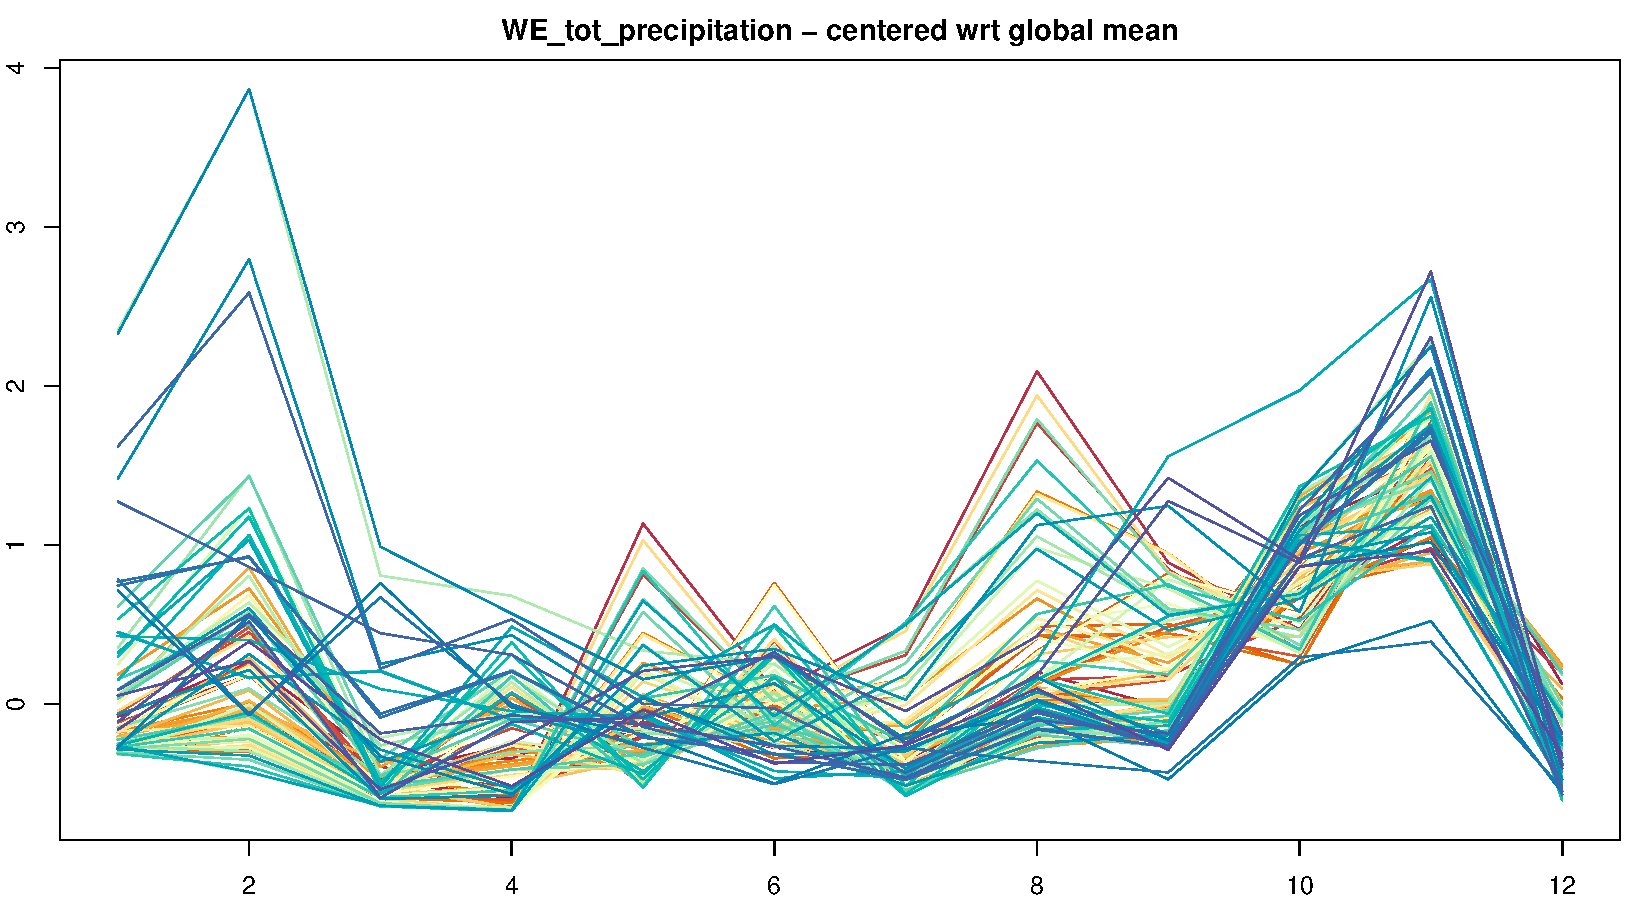
\includegraphics[width=1\linewidth]{Testing/Covariates/corollary images/WE_tot_precipitationcentered wrt global mean.pdf}
    % 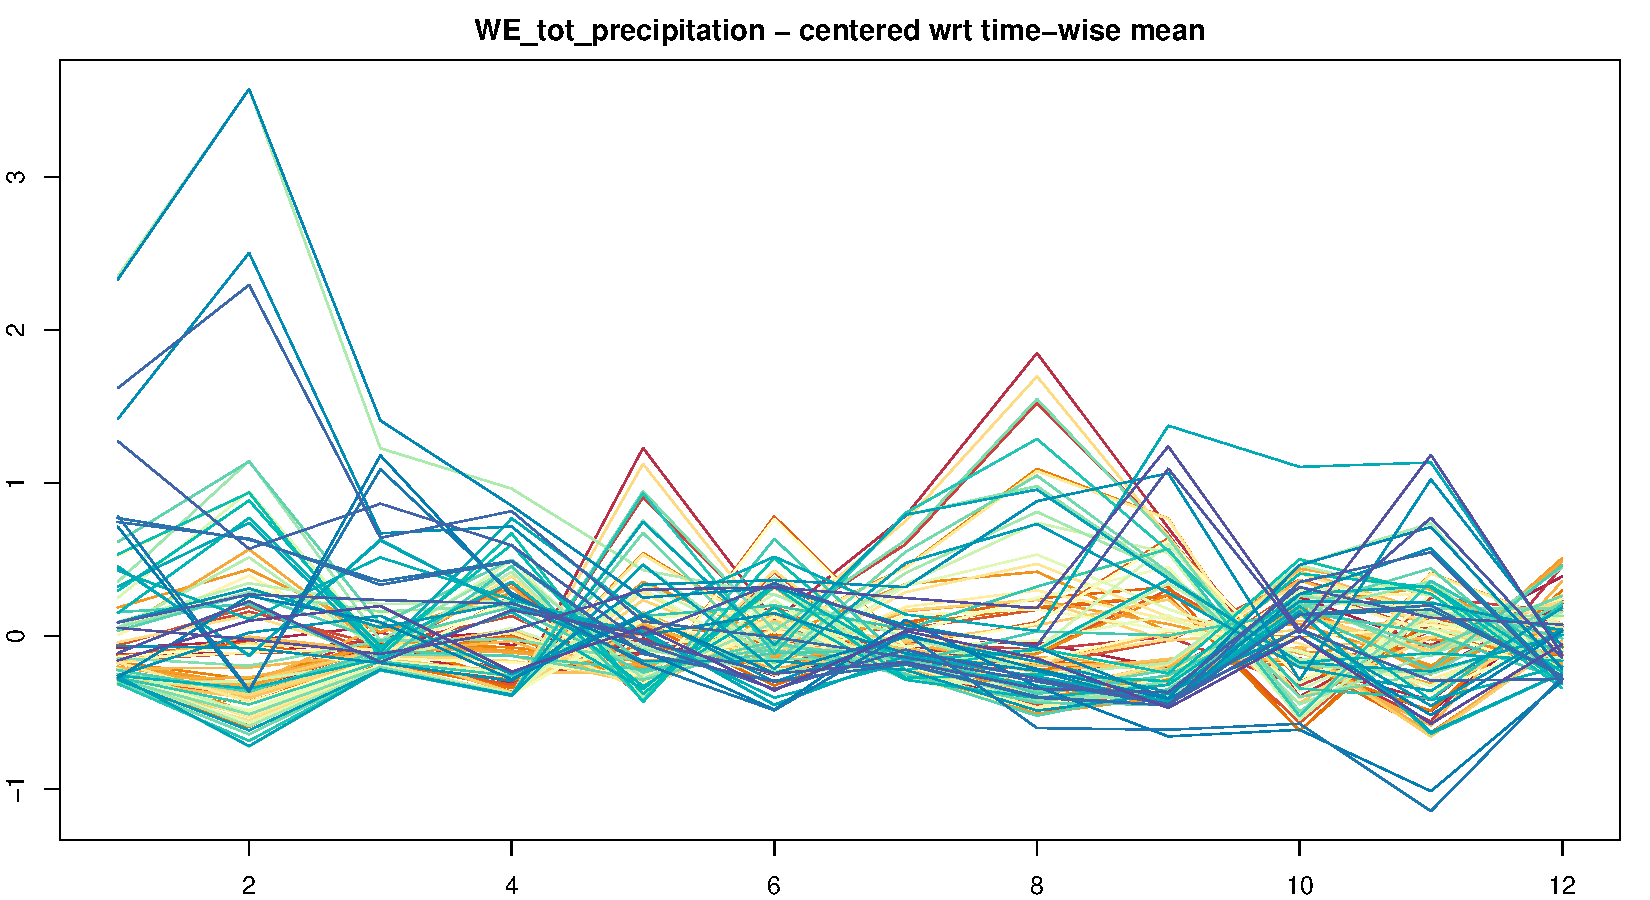
\includegraphics[width=1\linewidth]{Testing/Covariates/corollary images/WE_tot_precipitationcentered wrt time-wise mean.pdf}
    % 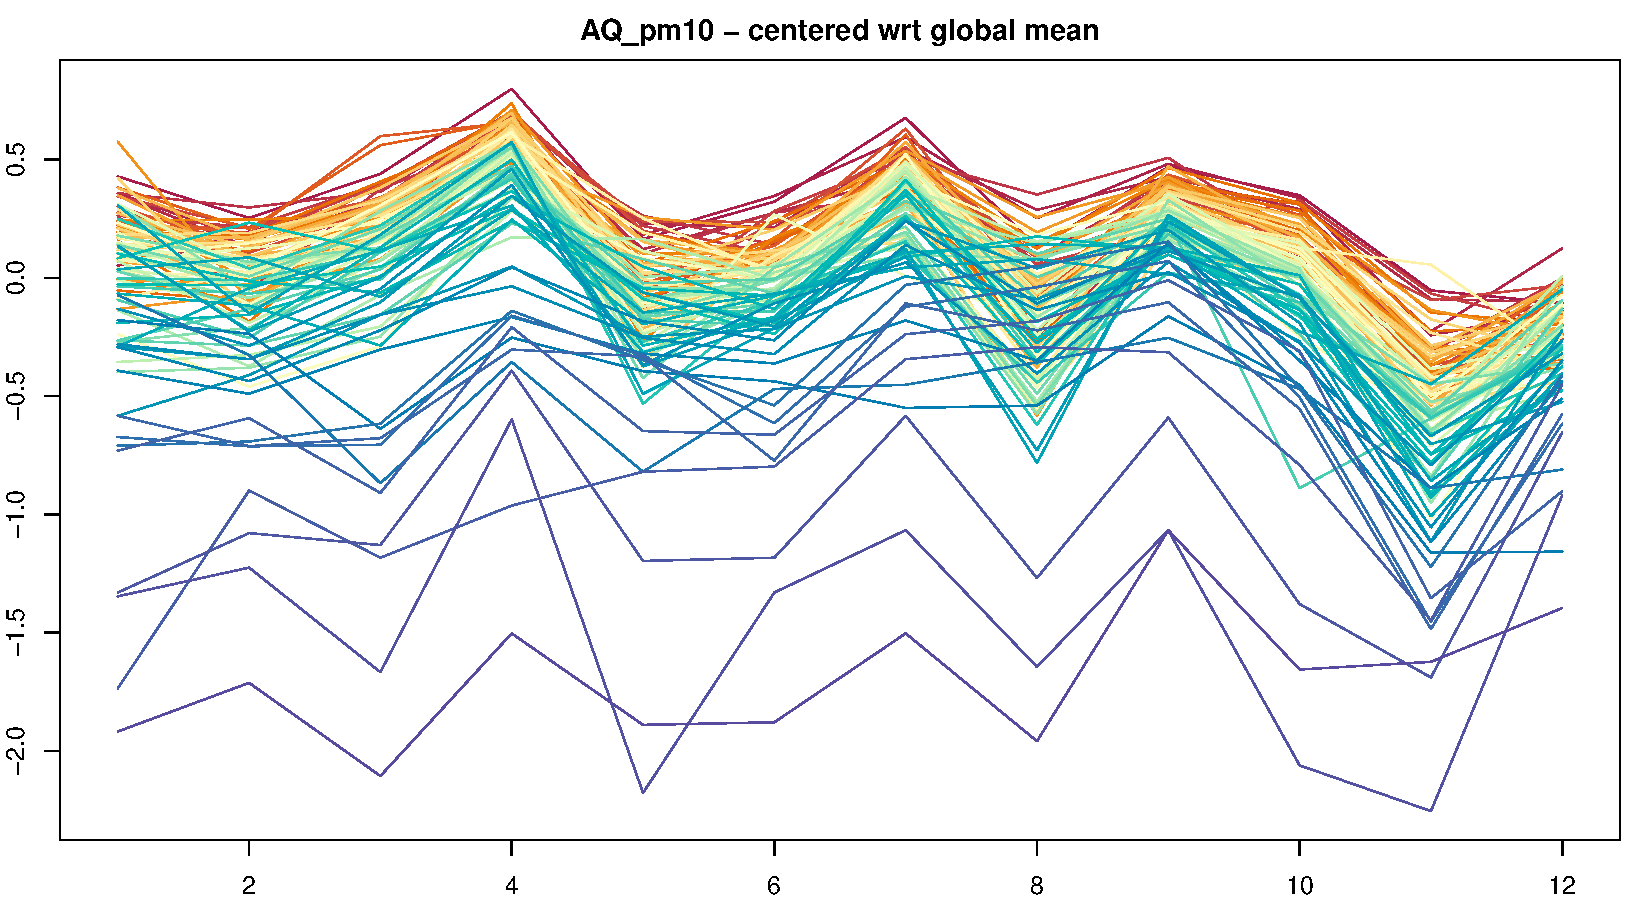
\includegraphics[width=1\linewidth]{Testing/Covariates/corollary images/AQ_pm10centered wrt global mean.pdf}
    % 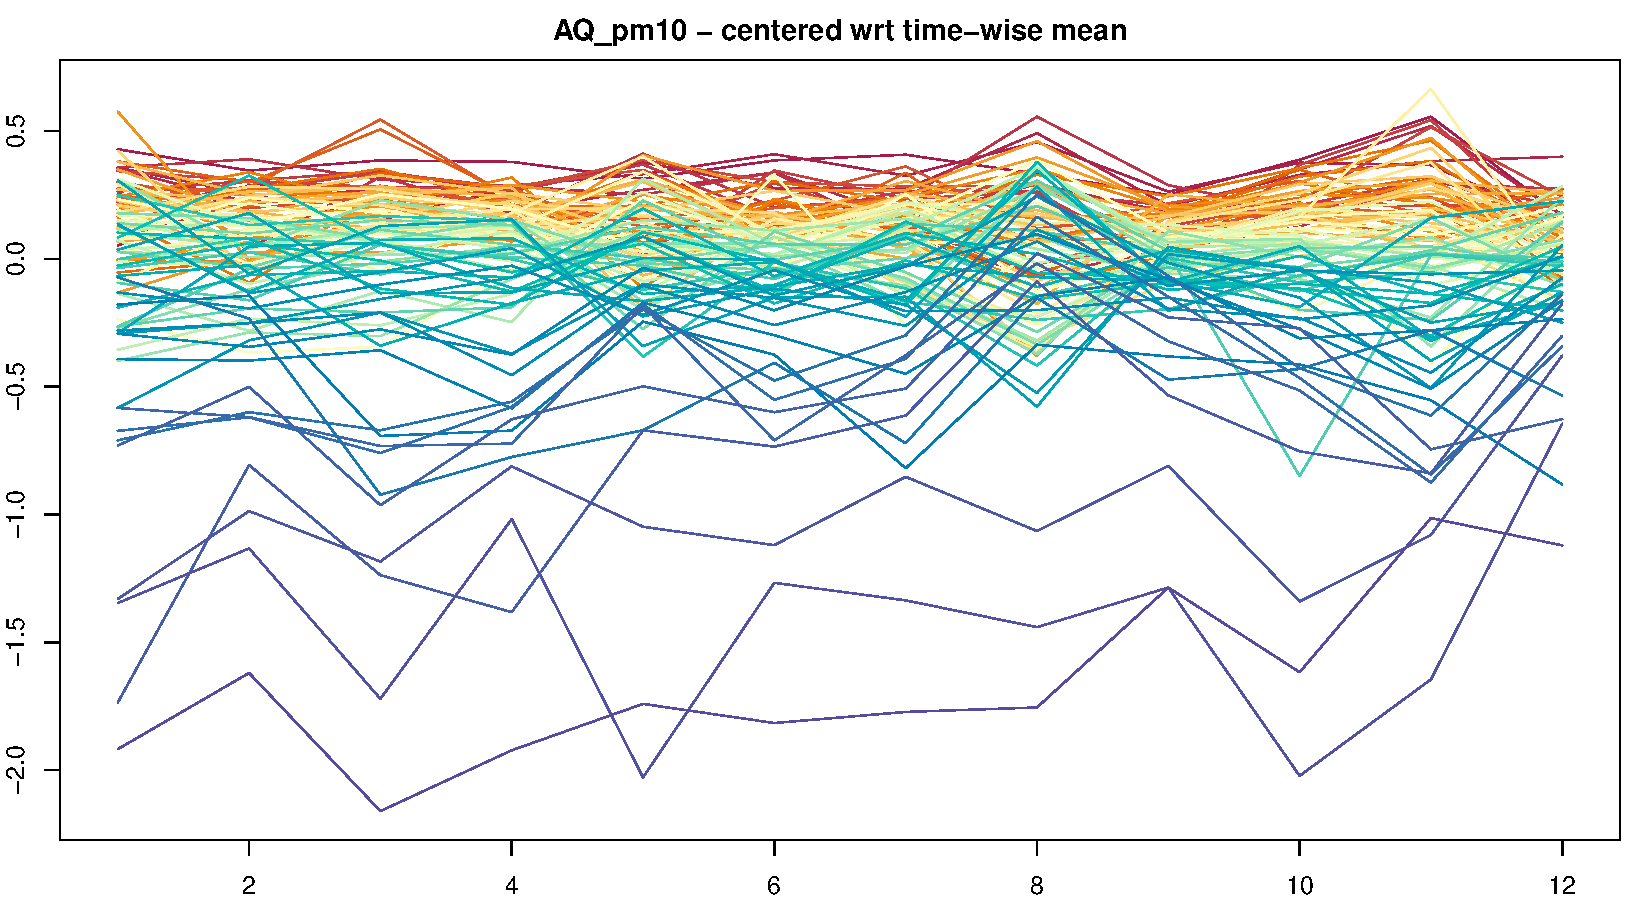
\includegraphics[width=0.8\linewidth]{Testing/Covariates/corollary images/AQ_pm10centered wrt time-wise mean.pdf}
    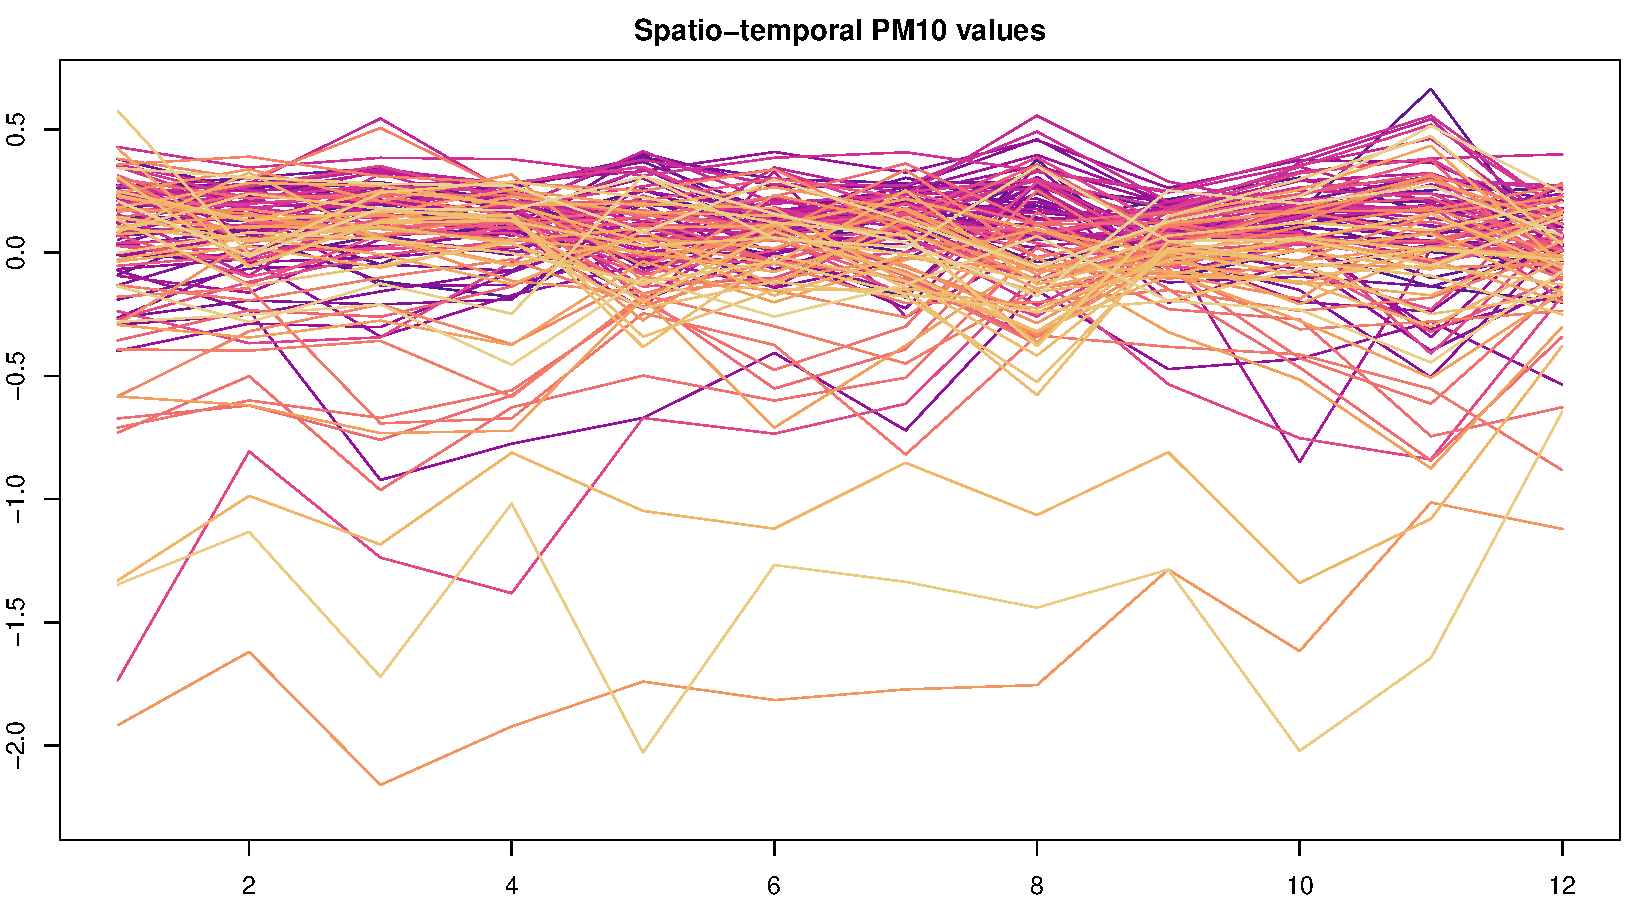
\includegraphics[width=0.8\linewidth]{imgs/test_2_spatial_data.pdf}
    % \caption[Comparison of the two mean centering methods]{Values of the target variable \tt{AQ\_pm10} adjusted using the global mean (top) and the time-wise mean (bottom). Coloring is based on the ranking of $\pmten$ values of the units according to their median, from highest (red) to lowest (blue).}
    \label{fig:different means conceptions PM10}
\end{figure}
\end{frame}

\begin{frame}{Real-world scenario}

    \begin{table}[!ht]
    % \caption[Comparison of CDRPM and JDRPM, real-world scenario]{Comparison between CDRPM and JDRPM fits and their associated algorithms, in the real-world scenario.}
    % Higher LPML and lower WAIC indicate a better fit.}
    \centering
     \resizebox{0.7\linewidth}{!}{%
    \begin{tabular}{cccc}
    \toprule
          % & \multicolumn{2}{c}{MSE using} & \multicolumn{2}{c}{Fit metrics} & \\
           % \cmidrule(lr){2-3}
           % \cmidrule(lr){4-5}
       % & MSE mean &  MSE median & LPML & WAIC & exec. time  \\
       % \midrule
       %  CDRPM &   0.0142   & 0.0149   & \textbf{ 694.81} & -1768.42 & 1h38m\\
       %  JDRPM & \textbf{0.0131}  & \textbf{0.0138}   & 624.91 & \textbf{-1898.05}  &  \textbf{48m}\\
       %  \bottomrule
              & MSE mean &  MSE median & execution time  \\
       \midrule
        CDRPM &   0.0142   & 0.0149  & 1h38m\\
        JDRPM & \textbf{0.0131}  & \textbf{0.0138}    &  \textbf{48m}\\
        \bottomrule
    \end{tabular}
    \label{tab: fits metrics space}
    }
\end{table}
\begin{figure}[!ht]
    \centering
    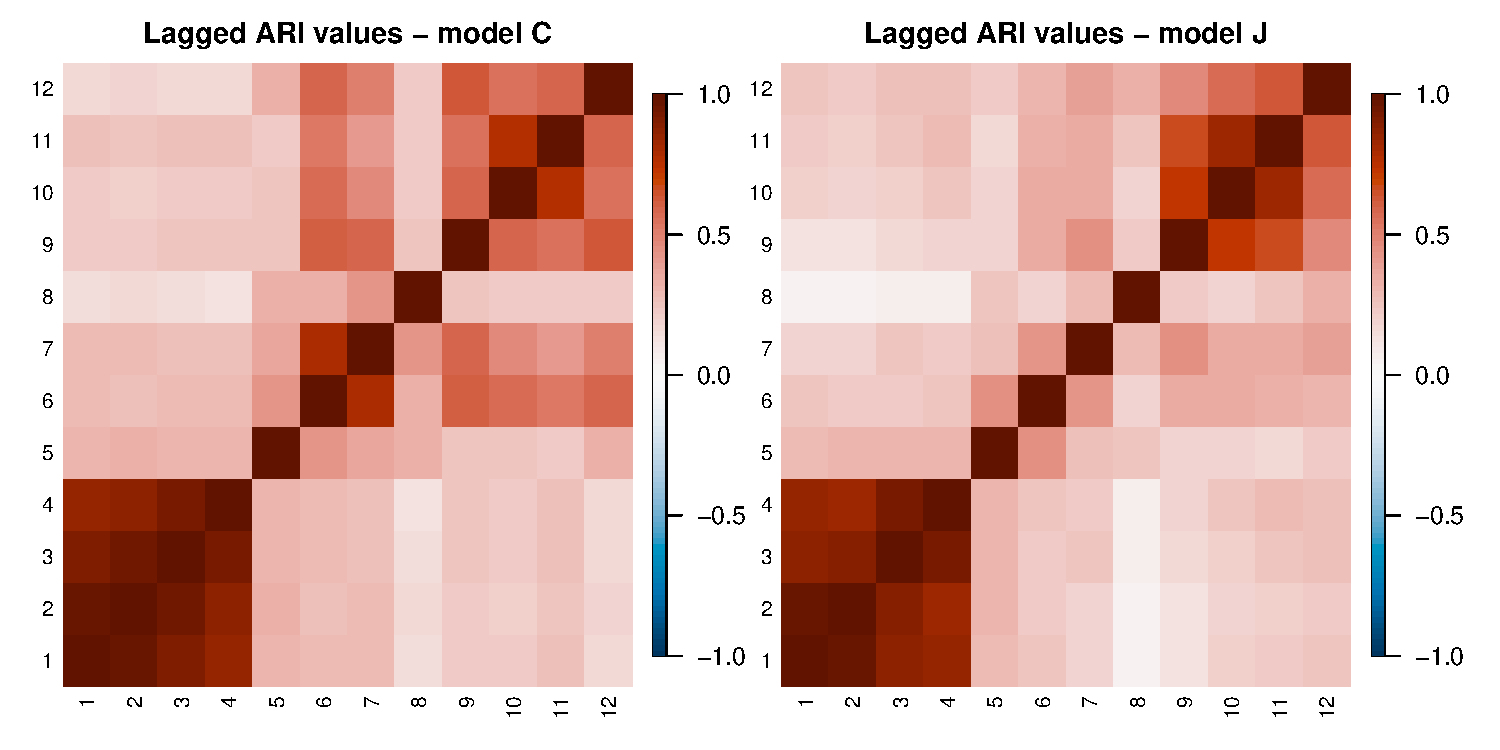
\includegraphics[width=0.9\linewidth]{Testing/Assessing correctness/space/ari.pdf}
    % \caption[Lagged ARI values of CDRPM and JDRPM, real-world scenario]{Lagged ARI values of CDRPM and JDRPM fits, in the real-world scenario.}
    \label{fig:ari space}
\end{figure}
\end{frame}

\begin{frame}{Real-world scenario}

% Clusters estimates were indeed similar: c
Computing the adjusted Rand index $\ari(\rho_{\text{JDRPM}}(t),\rho_{\text{CDRPM}}(t))$ for all time instants $t=1,\ldots,12$, we obtained a \alert{mean of 0.80} and a \alert{median of 0.86}, denoting a strong agreement between the clusters estimates.
    \begin{figure}
        \centering
        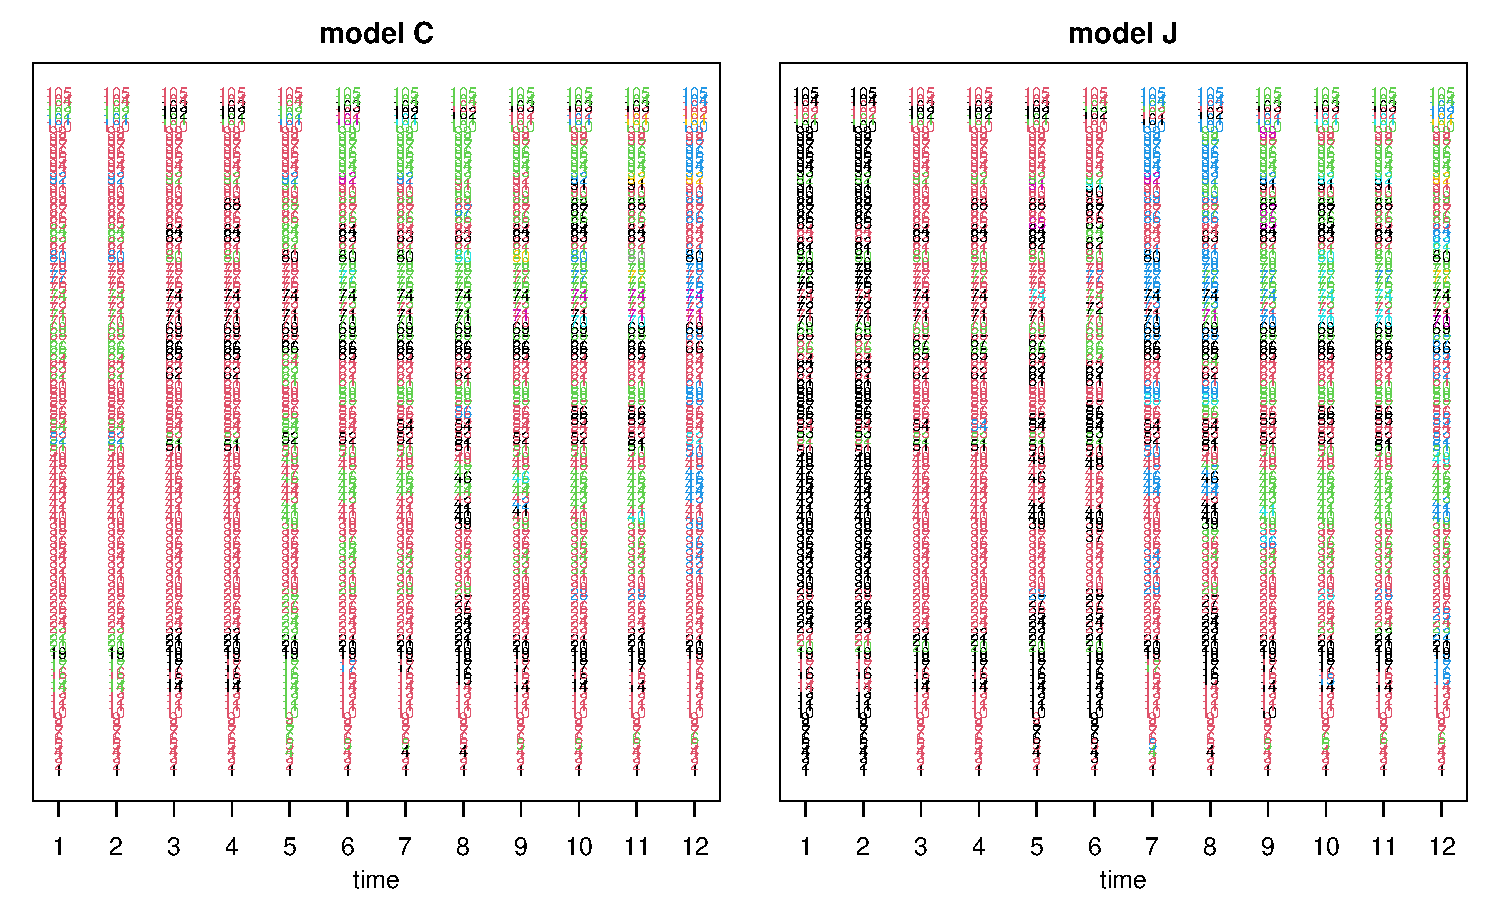
\includegraphics[width=0.8\linewidth,height=5.2cm]{imgs/partizioni_nums.pdf}
        % \caption{Enter Caption}
        \label{fig:enter-label}
    \end{figure}
\end{frame}

\subsection{Performance with missing values}
\begin{frame}{Performance with missing values}

We then replicated the analyses focusing on scenarios involving missing values, with the objective of investigating how the JDRPM performs in the absence of complete datasets and to determine whether it maintains effective performances under such conditions.\\[6pt]
Given the extent of missing values in the AgrImOnIA dataset \cite{agrimonia}, which was used for the spatio-temporal analysis, we opted to set 10\% of the values as missing (NAs). To implement this, we randomly selected $nT/10$ indexes from the sets $[1,\ldots,n]$ and $[1,\ldots,T]$ to identify all the pairs $(i,t)$ that would be designated as missing entries in the target variable $Y_{it}$. 
% The ability to handle missing data is an enhancement introduced by the JDRPM; therefore these studies cannot be repeated with the original CDRPM, which does not accept incomplete datasets.
\end{frame}


\begin{frame}{Simulated data}

\begin{table}[!ht]
    % \caption[Comparison of JDRPM, simulated data scenario, dataset with missing values]{Comparison of JDRPM fits, in the simulated data scenario, on a complete dataset and on a dataset with missing values.}
    \centering
     \resizebox{0.7\linewidth}{!}{%
    \begin{tabular}{cccccc}
    \toprule
          % & \multicolumn{2}{c}{MSE using} & \multicolumn{2}{c}{Fit metrics} & \\
           % \cmidrule(lr){2-3}
           % \cmidrule(lr){4-5}
            & MSE mean &  MSE median & LPML & WAIC & exec. time  \\
           % & mean &  median & LPML & WAIC & execution time  \\
           \midrule
        full data& 1.2634 & 1.2034  & -223.36 & 393.97  &  13s \\
        NA data &   1.4721   & 1.2101 & -236.93 & 401.44 & 13s\\
        \bottomrule
    \end{tabular}
    \label{tab: fits metrics no space julias na full}
    }
\end{table}
\begin{figure}[!ht]
    \centering
    % \includegraphics[width=1\linewidth]{Testing/NA data/no space NA/test_1_generated_data.pdf}
    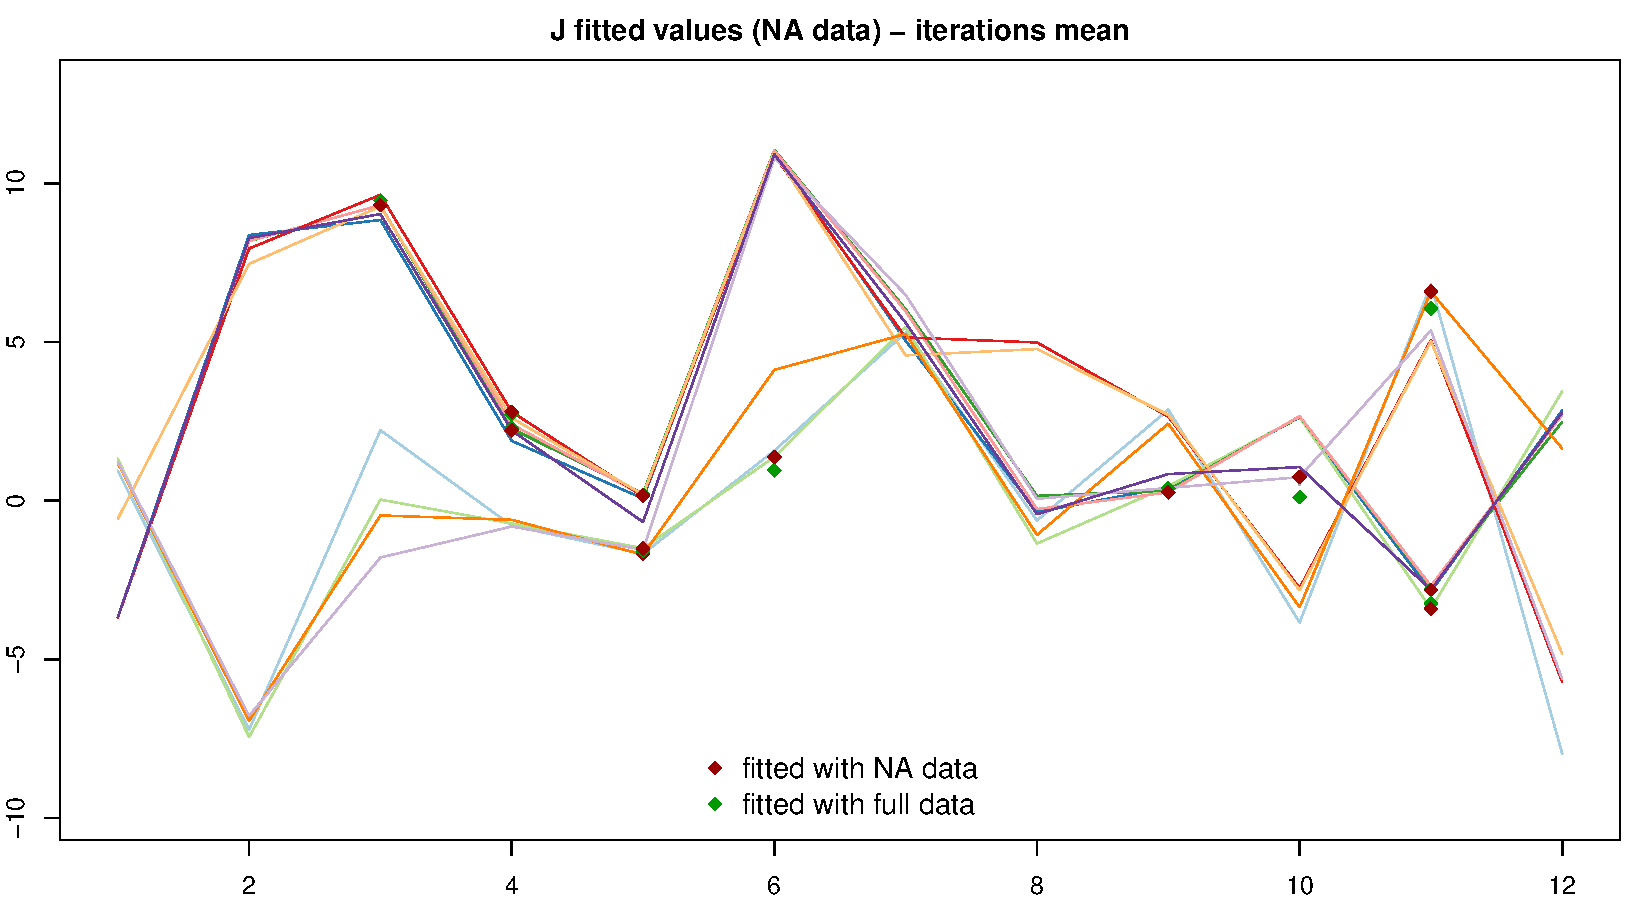
\includegraphics[width=0.85\linewidth]{Testing/NA data/no space NA/J_mean_prediction.pdf}
    % \caption[Fitted values of JDRPM, simulated data scenario, dataset with missing values]{Fitted values of JDRPM fit, in the simulated data scenario, with missing values in the target variable. Special square markers are devoted to the data points which were missing, highlighting the gaps between the fitted values on the full dataset (green) and the fitted values on the dataset with missing values (red).}
    \label{fig: target values estimates no space NA}
\end{figure}
\end{frame}

\begin{frame}{Simulated data}

\begin{figure}[!ht]
    \centering
    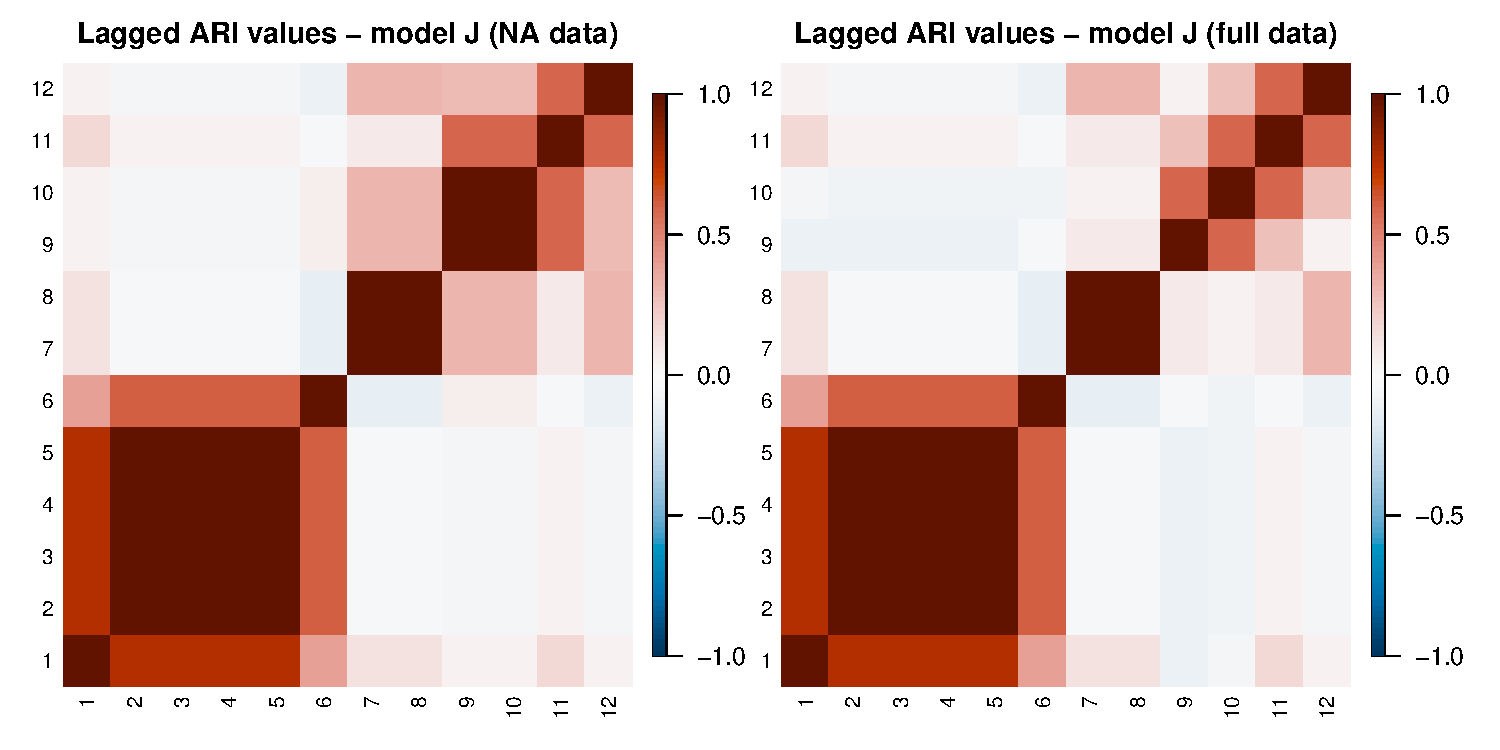
\includegraphics[width=1\linewidth]{Testing/NA data/no space NA/ari.pdf}
    % \caption[Lagged ARI values of JDRPM, simulated data scenario, dataset with missing values]{Lagged ARI values of JDRPM fits, in the simulated data scenario, on a dataset with missing values.}
    \label{fig:ari no space NA}
\end{figure}
\end{frame}

\begin{frame}{Simulated data}
    
\begin{figure}[!ht]
    \centering
    % 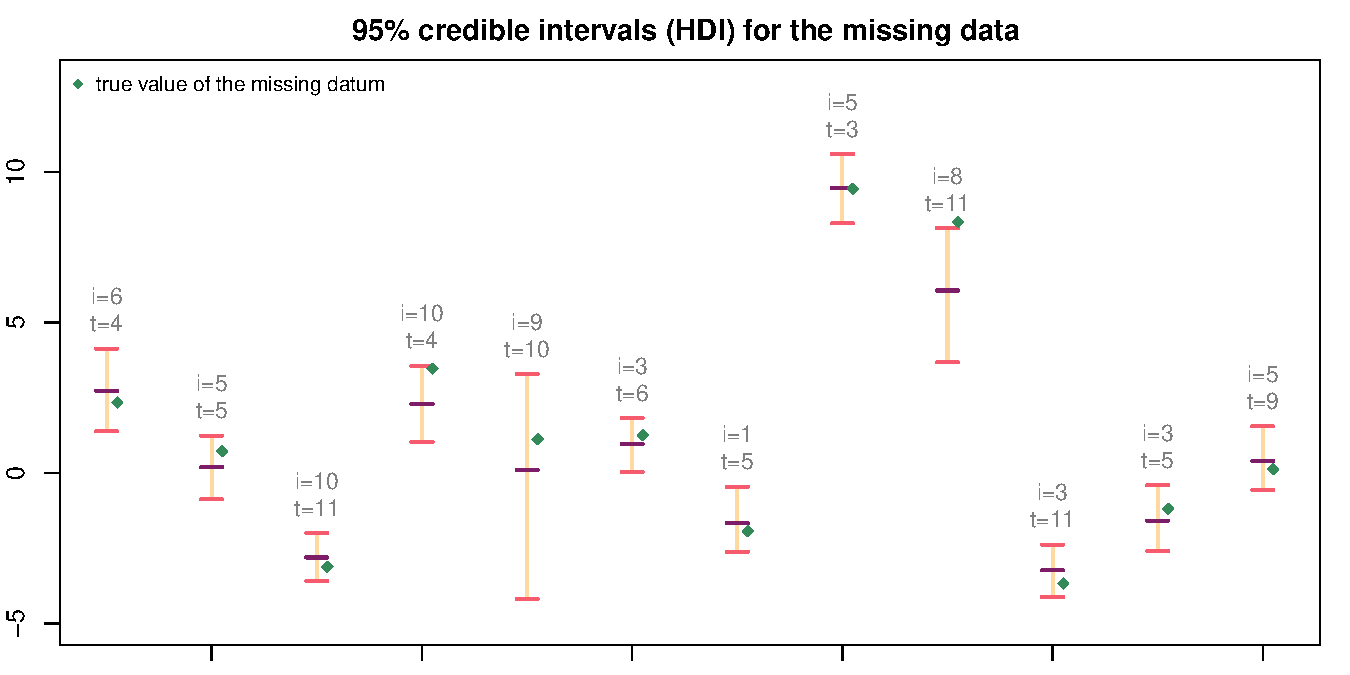
\includegraphics[width=1\linewidth]{Testing/NA data/no space NA/target_only_NA_CIs.pdf}
    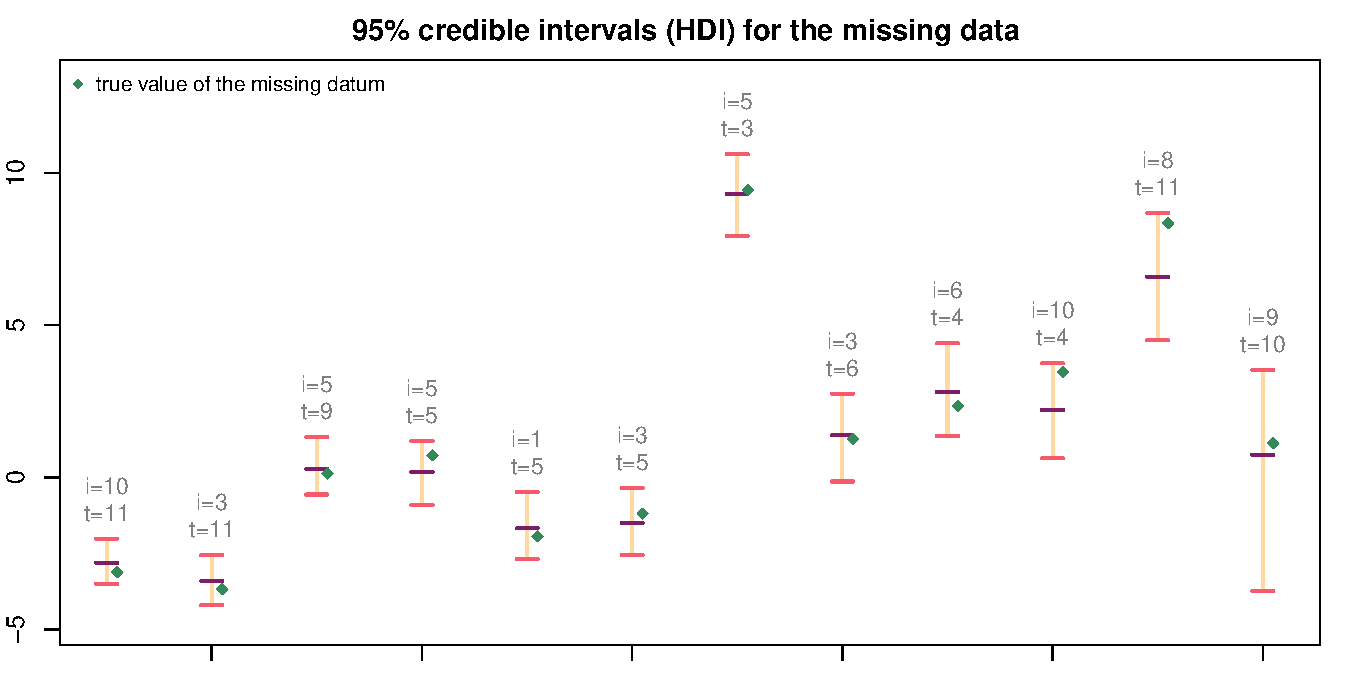
\includegraphics[width=1\linewidth]{Testing/NA data/no space NA/target_only_NA_CIs_SORTED.pdf}
    % \caption[Credible intervals of JDRPM, simulated data scenario, dataset with missing values]{Credible intervals, computed with the highest density interval (HDI) method at a 95\% confidence, for the fitted values of the missing units in the JDRPM fit, in the simulated data scenario, on a dataset with missing values. In gray are reported the indexes of units $i$ and time instants $t$ which where missing, while green dots refer to the true values of the missing data.}
    \label{fig: CIs target only}
\end{figure}
\end{frame}

\begin{frame}{Real-world scenario}

    \begin{table}[!ht]
    % \caption[Comparison of JDRPM, real-world scenario, dataset with missing values]{Comparison of JDRPM fits, in the real-world scenario, on a complete dataset and on a dataset with missing values.}
    \centering
     \resizebox{0.7\linewidth}{!}{%
    \begin{tabular}{cccccc}
    \toprule
          % & \multicolumn{2}{c}{MSE using} & \multicolumn{2}{c}{Fit metrics} & \\
           % \cmidrule(lr){2-3}
           % \cmidrule(lr){4-5}
            & MSE mean &  MSE median & LPML & WAIC & exec. time  \\
           % & mean &  median & LPML & WAIC & execution time  \\
           \midrule 
        full data & 0.0131  & 0.0138   & 624.91 & -1898.05  &  48m \\
        NA data & 0.0160 &  0.0170  &  502.86 & -1793.64 & 43m\\
        % \midrule
        % & & & & mean & median \\
        % \multicolumn{4}{c}{$\ari(\rho_{\text{JDRPM\_NA}}(t),\rho_{\text{CDRPM\_full}}(t))$} & 1 & 2 \\
        \bottomrule
    \end{tabular}
    \label{tab: fits metrics space julias na full}
    }
\end{table}
\begin{figure}[!ht]
    \centering
    % \includegraphics[width=1\linewidth]{Testing/NA data/no space NA/test_1_generated_data.pdf}
    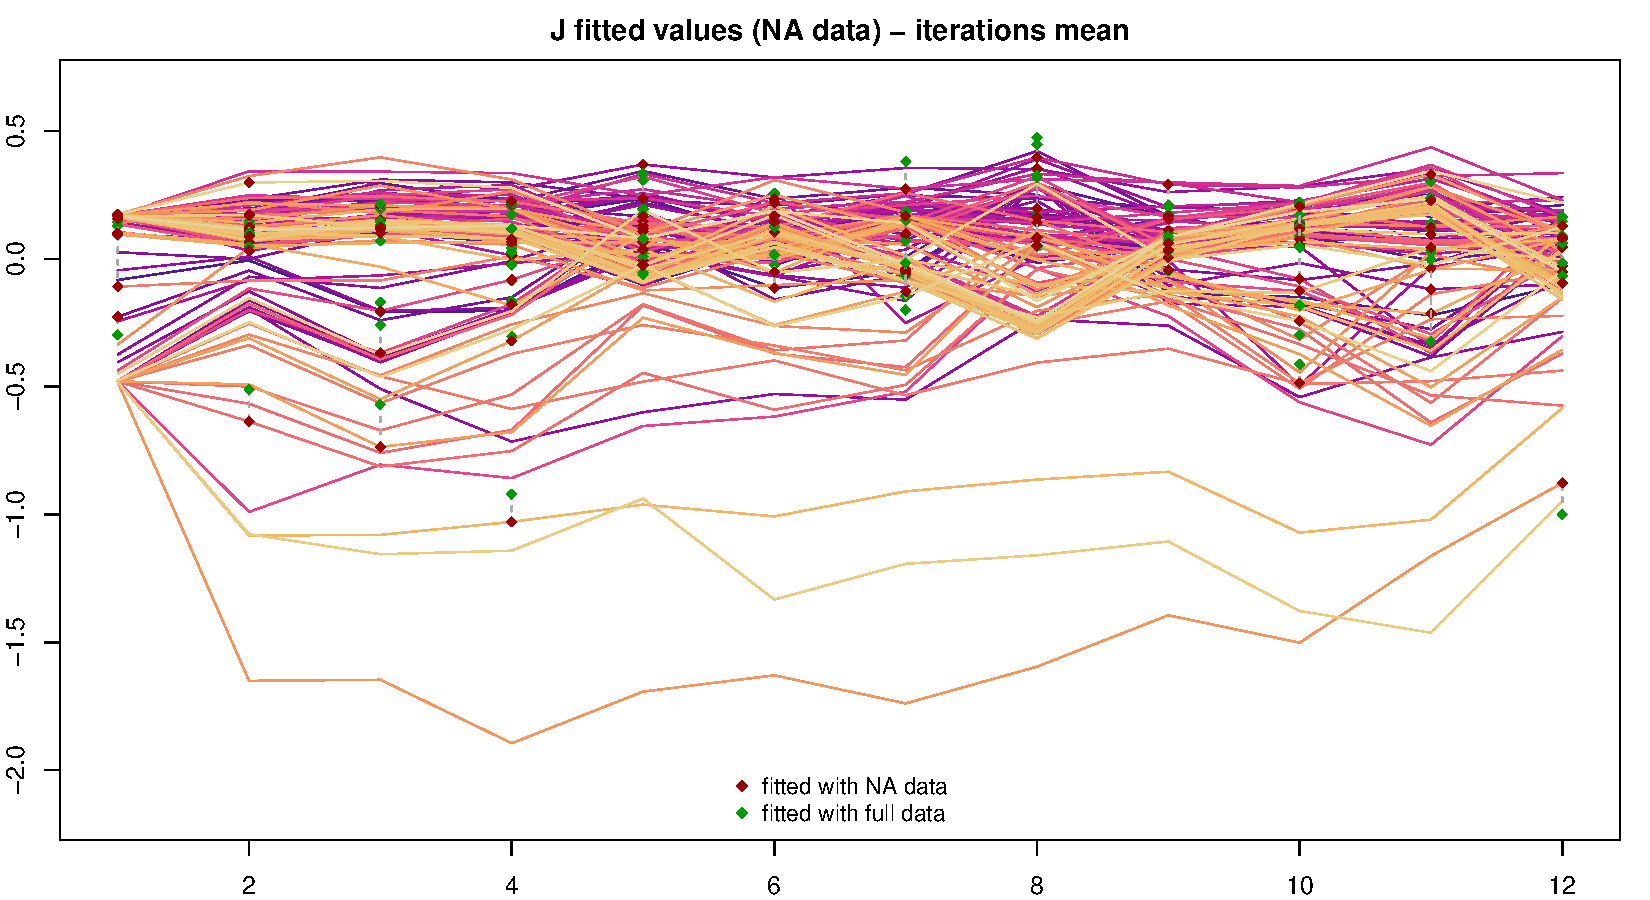
\includegraphics[width=0.85\linewidth]{Testing/NA data/space/J_mean_prediction.pdf}
    % \caption[Fitted values of JDRPM, real-world scenario, dataset with missing values]{Fitted values of JDRPM fit, in the real-world scenario, on a dataset with missing values. Special square markers are devoted to the data points which were missing, highlighting the gaps between the fitted values on the full dataset (green) and the fitted values on the dataset with missing values (red).}
    \label{fig: target values estimates space NA}
\end{figure}
\end{frame}

\begin{frame}{Real-world scenario}

    \begin{figure}[!ht]
    \centering
    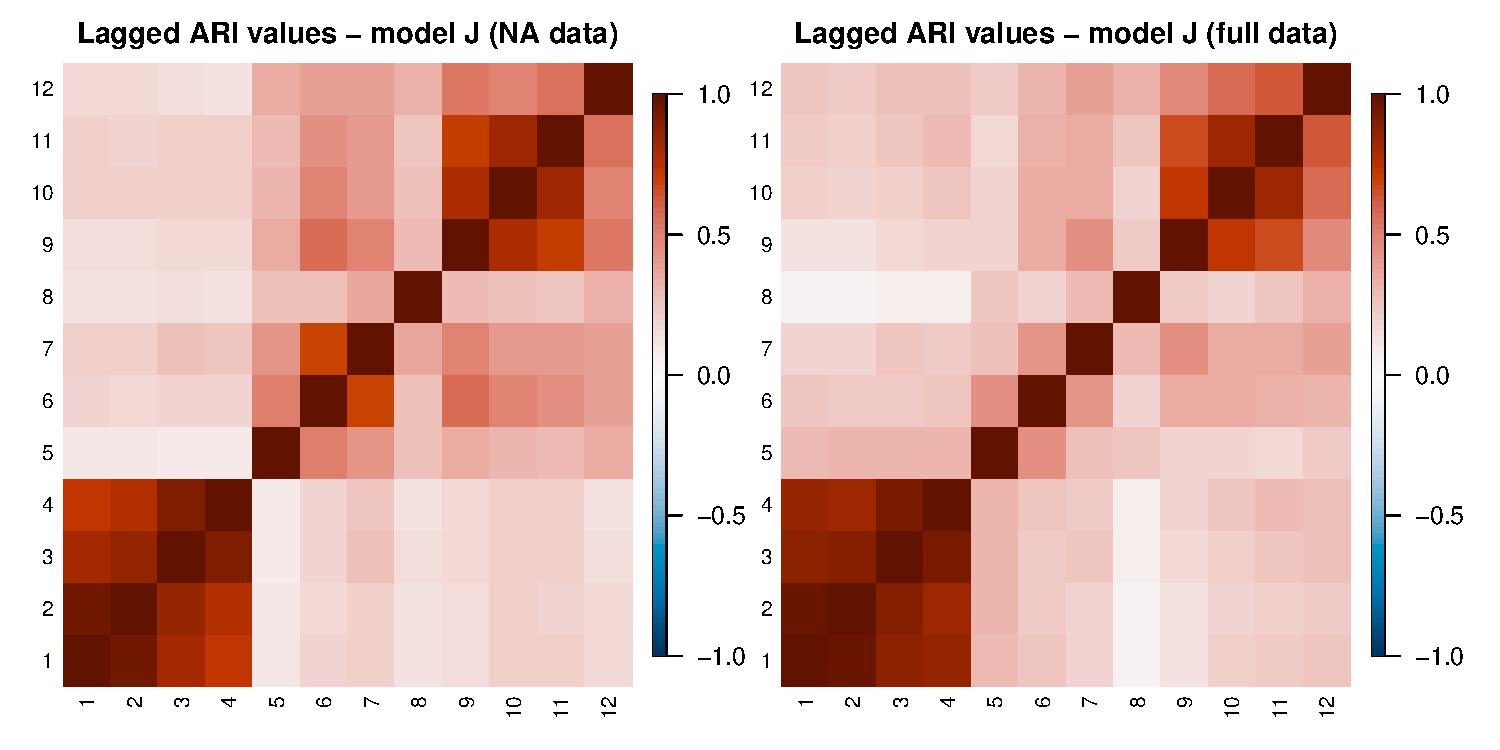
\includegraphics[width=1\linewidth]{Testing/NA data/space/ari.pdf}
    % \caption[Lagged ARI values of JDRPM, real-world scenario, dataset with missing values]{Lagged ARI values of JDRPM fits, in the real-world scenario, on a dataset with missing values.}
    \label{fig: ari space na}
\end{figure}
\end{frame}

\begin{frame}{Real-world scenario}

    \begin{figure}
        \centering
        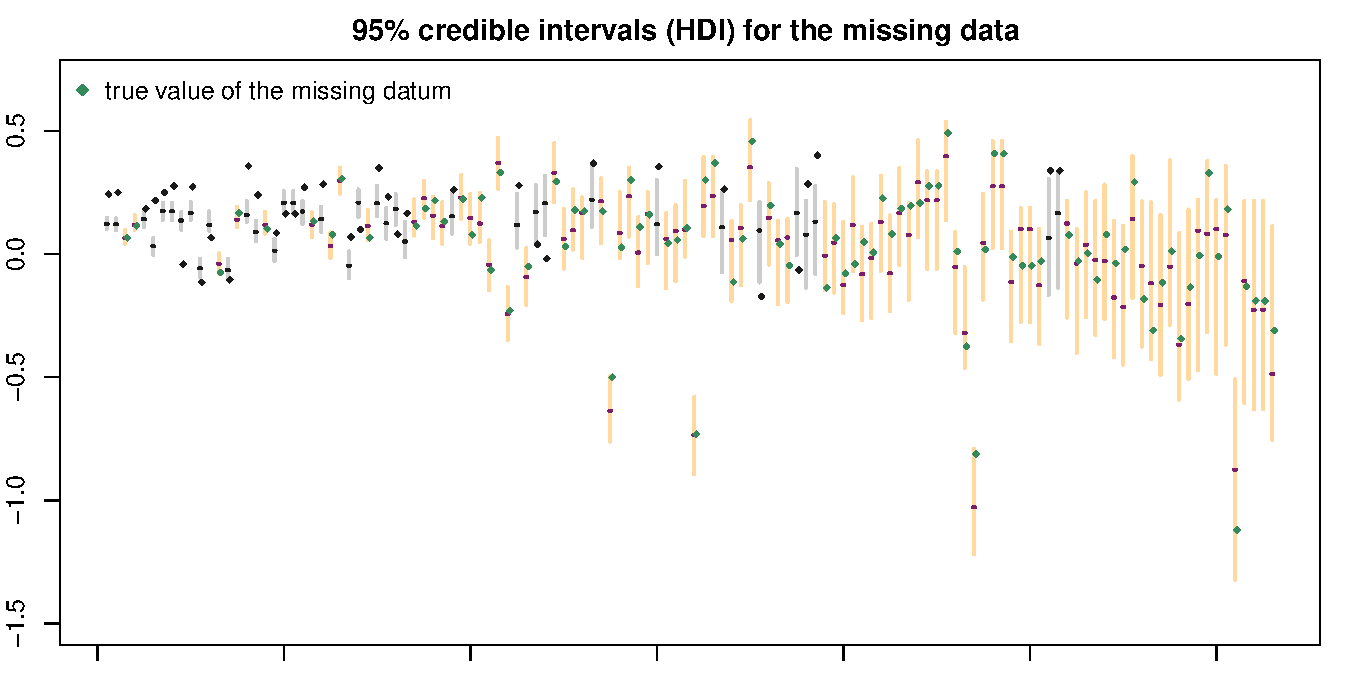
\includegraphics[width=1\linewidth]{imgs/NA_SORTED_space_pure.pdf}
        \caption{74\% of the true values lie within the credible intervals.}
        \label{fig:enter-label}
    \end{figure}
    % \footnotesize{74\% of the true values lie within the credible intervals}\normalsize
\end{frame}


\subsection{Effects of the covariates}
\begin{frame}{Effects of the covariates}
% the effects of including covariates in the likelihood and including covariates in the prior. 
% For the upcoming fits, all included covariates underwent the same time-wise correction applied to the target variable $\pmten$, as outlined before.

We then conducted several experiments to explore the key advancement introduced by the JDRPM: the inclusion of covariates. \\[6pt]
Given their distinctly different purposes, we studied separately their effects:
\vspace{-5mm}
\begin{itemize}
    \item covariates in the likelihood are expected to improve the estimation quality of the target variable $Y_{it}$ and the associated model parameters $\implies$ context of the spatio-temporal experiments, with missing data
    \item covariates in the prior are expected to improve the accuracy and interpretability clusters estimates $\implies$ context of the spatio-temporal experiments
\end{itemize}
\end{frame}


% \begin{frame}{Covariates in the likelihood}
% Covariates in the likelihood have the main objective of improving the fitted estimates of the target variable $Y_{it}$ through the insertion of the additional information from the regression term.\\[6pt]
% To this end, we repeated the \alert{spatio-temporal experiments \emph{on missing data}}, but this time \alert{with covariates in the likelihood}.
% % To this end, we repeated the spatio-temporal experiments on missing data, to investigate the effect of covariates in the likelihood. 
% % Indeed, such fit yielded more accurate fitted estimates. 
% \end{frame}

\begin{frame}{Covariates in the likelihood}
\begin{table}[!ht]
    % \caption[Comparison of JDRPM, real-world scenario, covariates in the likelihood, dataset with missing values]{Comparison of JDRPM fits, in the real-world scenario, with and without the inclusion of covariates in the likelihood, on a complete dataset and on a dataset with missing values.}
    % The MSE columns refer to the accuracy between the fitted values generated by the models (estimated by taking the mean and the median of the returned 4000 iterates) and the true values of the target variable. Higher LPML and lower WAIC indicate a better fit.
    \centering
        \resizebox{0.7\linewidth}{!}{%
    \begin{tabular}{cccccc}
    \toprule
          % & \multicolumn{2}{c}{MSE using} & \multicolumn{2}{c}{Fit metrics} & \\
           % \cmidrule(lr){2-3}
           % \cmidrule(lr){4-5}
            & MSE mean &  MSE median & LPML & WAIC & exec. time  \\
           % & mean &  median & LPML & WAIC & execution time  \\
           \midrule 
        % full data & 0.0131  & 0.0138   & 624.91 & -1898.05  &  \textbf{48m} \\
        % full data + Xlk & \textbf{0.0112}  & \textbf{0.0113}   & \textbf{778.96} & \textbf{-2029.84}  &  56m \\
        % \midrule
         full data & 0.0131  & 0.0138   & 624.91 & -1898.05  &  48m \\
        NA data & 0.0160 &  0.0170  &  502.86 & -1793.64 & \textbf{43m}\\
        NA data + Xlk & \textbf{0.0127} &  \textbf{0.0130}  & \textbf{625.81 }& \textbf{-1902.74} & 58m\\
        % \midrule
        % & & & & mean & median \\
        % \multicolumn{4}{c}{$\ari(\rho_{\text{JDRPM\_NA}}(t),\rho_{\text{CDRPM\_full}}(t))$} & 1 & 2 \\
        \bottomrule
    \end{tabular}
    \label{tab: fits metrics space julias na full xlk}
    }
\end{table}
    \begin{figure}[!ht]
    \centering
    % 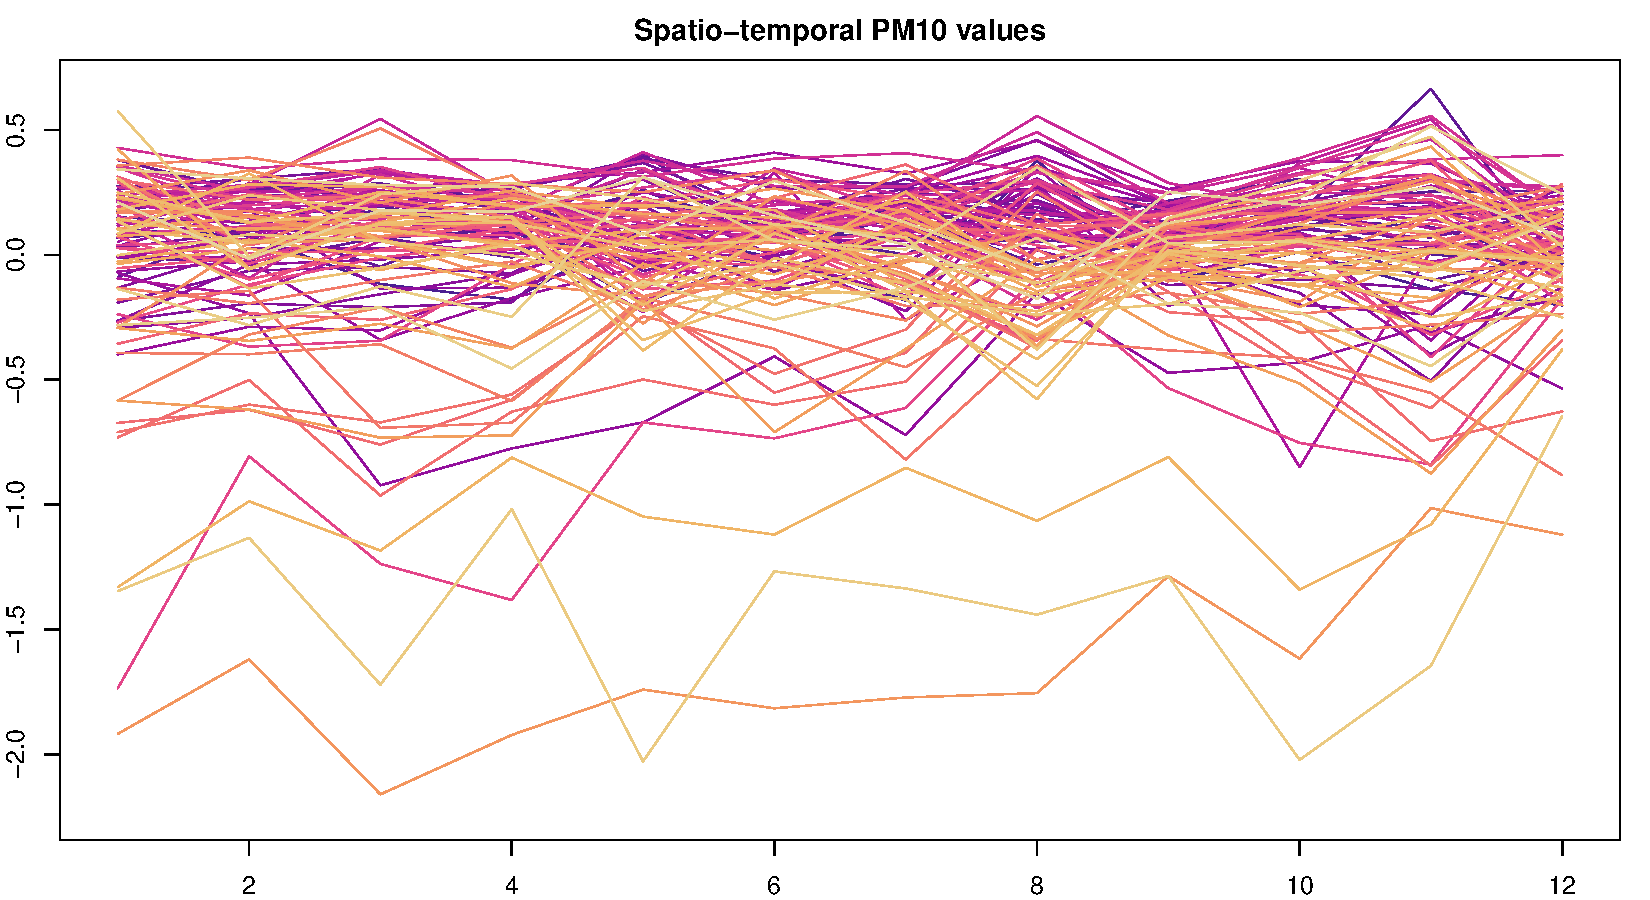
\includegraphics[width=1\linewidth]{Testing/Covariates/NA lk improvement/test_2_spatial_data.pdf}
    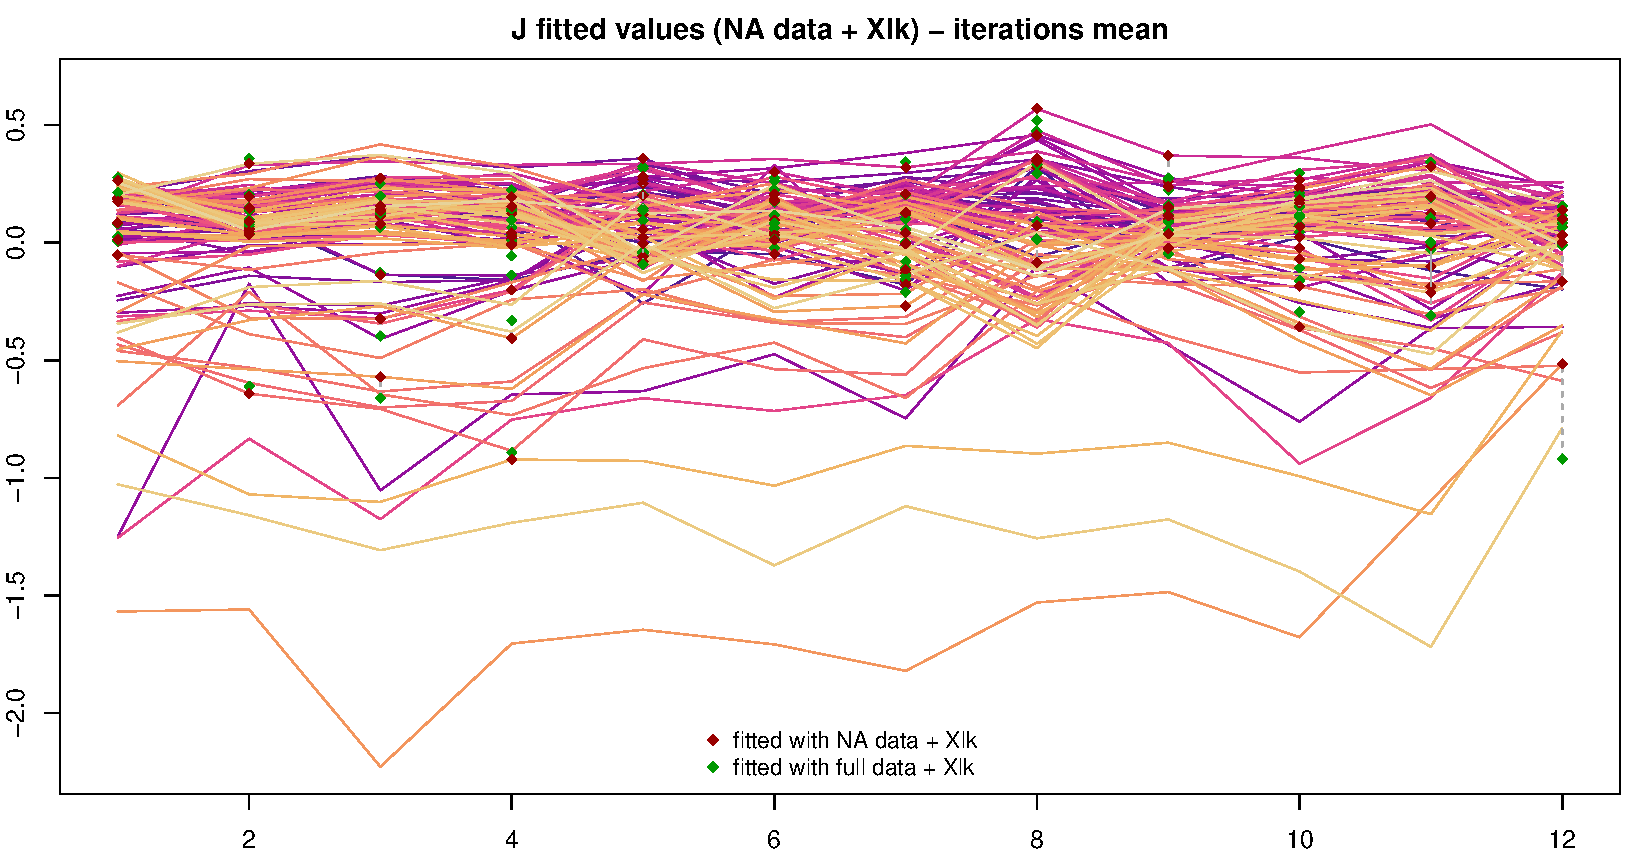
\includegraphics[width=0.9\linewidth]{Testing/Covariates/NA lk improvement/J_mean_prediction_NA.pdf}
    % \includegraphics[width=1\linewidth]{Testing/Covariates/NA lk improvement/J_mean_prediction_full.pdf}
    % \caption[Target and fitted values of JDRPM fits, target plus space values, NA dataset, with covariates in the likelihood]{Target and fitted values of the JDRPM fits with target plus space values, on the NA and full dataset, to see the effects of the insertion of covariates in the likelihood.}
    \label{fig: all NA fitted values tests}
\end{figure}
\end{frame}

\begin{frame}{Covariates in the likelihood}
\begin{figure}[!p]
    \centering
    % \includegraphics[clip, trim=0pt 0pt 0pt 15pt,width=1\linewidth]{Testing/Covariates/better likelihood plots/LINES_beta_TR_plus_CIJDRPM - full data + Xlk.pdf}
    \includegraphics[clip, trim=0px 25.97cm 0px 15px, width=1\linewidth]{Testing/Covariates/better likelihood plots/up_LINES_beta_TR_plus_CIJDRPM - full data + Xlk.pdf}\\
    \includegraphics[clip, trim=0px 0cm 0px 26.6cm, width=1\linewidth]{Testing/Covariates/better likelihood plots/up_LINES_beta_TR_plus_CIJDRPM - full data + Xlk.pdf}
    % \caption[Regression vector of JDRPM, covariates in the likelihood, full dataset]{Regression vector $\vec{\beta}_t$ of JDRPM fit, in the real-world scenario, for the $p=6$ covariates inserted in the likelihood, on the full spatio-temporal dataset, with trace plots (left) and 95\% credible intervals (right) computed with the highest density interval (HDI) method.}
    \label{fig: lk regressor altitude and friends full}
\end{figure}
\end{frame}

% \begin{frame}{Covariates in the prior}
% Covariates in the prior have the main objective of improving clusters estimates through the insertion of their additional information.\\[6pt]
% % Indeed, JDRPM fit with covariates turned out to be with more accurate and interpretable results.
% To this end, we repeated the \alert{spatio-temporal experiments}, but this time \alert{with covariates in the prior}.
% \end{frame}

\begin{frame}{Covariates in the prior}
    
\begin{table}[!ht]
    % \caption[Comparison of CDRPM and JDRPM, real-world scenario, covariates in the prior]{Comparison between CDRPM and JDRPM fits and their associated algorithms, in the real-world scenario, with and without covariates in the prior.}
    \centering
    \resizebox{0.7\linewidth}{!}{%
    \begin{tabular}{cccccc}
    \toprule
          % & \multicolumn{2}{c}{MSE using} & \multicolumn{2}{c}{Fit metrics} & \\
           % \cmidrule(lr){2-3}
           % \cmidrule(lr){4-5}
           & MSE mean &  MSE median & LPML & WAIC & exec. time  \\
           % & mean &  median & LPML & WAIC & execution time  \\
           \midrule
        CDRPM &   0.0142   & 0.0149   &  694.81 & -1768.42 & 1h38m\\
        JDRPM & 0.0131  & 0.0138   & 624.91 & -1898.05  &  \textbf{48m}\\
        % \midrule
        JDRPM + Xcl & \textbf{0.0126}  & \textbf{0.0135}  & \textbf{677.71} & \textbf{-1969.76}  &  1h20m\\
        % JDRPM t+Xcl+Xlk & 0.0126  & 0.0135  & 742.72 & -1759.15  &  35m\\
        \bottomrule
    \end{tabular}
    \label{tab: fits metrics space all with also Xcl}
    }
\end{table}
\begin{figure}[!ht]
    \centering
    \includegraphics[width=0.9\linewidth]{Testing/Covariates/in clustering/ari_sp_vs_Xcl.pdf}
    % \caption[Lagged ARI values of JDRPM fits, in the real-world scenario, with covariates in the prior.]{Lagged ARI values of CDRPM and JDRPM fits, in the real-world scenario, with covariates in the prior.}
    \label{fig: Jxcl ari values plot}
\end{figure}
\end{frame}


% \begin{frame}
%     \begin{figure}[!ht]
%     \centering
%     \includegraphics[width=0.84\linewidth]{Testing/Covariates/in clustering/space C/CDRPM target + space_t09.pdf}
% %     \label{fig: summary fits battle}
% % \end{figure}
% % \end{frame}
% % \begin{frame}{Covariates in the prior}
%     % \begin{figure}[!ht]
%     % \centering
%     % \includegraphics[width=0.84\linewidth]{Testing/Covariates/in clustering/space J/JDRPM target + space_t09.pdf}
%      \includegraphics[width=0.84\linewidth]{Testing/Covariates/in clustering/space J Xcl/JDRPM target + space + Xcl_t09.pdf}
%     \label{fig: summary fits battle}
% \end{figure}
% \end{frame}

% % \begin{frame}{Covariates in the prior}
% %     \begin{figure}[!ht]
% %     \centering
% %     % \footnotesize{(a)}\includegraphics[width=1\linewidth]{Testing/Covariates/in clustering/space C/CDRPM target + space_t09.pdf}
% %     \includegraphics[width=1\linewidth]{Testing/Covariates/in clustering/space J Xcl/JDRPM target + space + Xcl_t09.pdf}
% %     % \footnotesize{(c)}\includegraphics[width=1\linewidth]{Testing/Covariates/in clustering/space J Xcl/JDRPM target + space + Xcl_t09.pdf}
% %     \label{fig: summary fits battle}
% % \end{figure}
% % \end{frame}

% \begin{frame}
%     \begin{figure}
%         \centering
%         \includegraphics[width=0.7\linewidth]{imgs/WE_wind_speed_10m_max_CDRPM_sorted_ZOOM.pdf}
%         \includegraphics[width=0.7\linewidth]{imgs/WE_wind_speed_10m_max_JDRPM_sorted_ZOOM.pdf}
%         \label{fig:enter-label}
%     \end{figure}
% \end{frame}


%%%%%%%%%%%%%%%%%%% SINGOLE
\begin{frame}{Covariates in the prior}
    \begin{figure}[!ht]
    \centering
    \includegraphics[width=1\linewidth]{Testing/Covariates/in clustering/space C/CDRPM target + space_t09.pdf}
    \caption{CDRPM spatially-informed fit.}
     % \includegraphics[width=1\linewidth]{Testing/Covariates/in clustering/space J Xcl/JDRPM target + space + Xcl_t09.pdf}
    \label{fig: summary fits battle}
\end{figure}
\end{frame}
% \begin{frame}{Covariates in the prior}
%     \begin{figure}[!ht]
%     \centering
%     \includegraphics[width=1\linewidth]{Testing/Covariates/in clustering/space J/JDRPM target + space_t09.pdf}
%     \caption{JDRPM spatially-informed fit.}
%      % \includegraphics[width=1\linewidth]{Testing/Covariates/in clustering/space J Xcl/JDRPM target + space + Xcl_t09.pdf}
%     \label{fig: summary fits battle}
% \end{figure}
% \end{frame}
\begin{frame}{Covariates in the prior}
    \begin{figure}[!ht]
    \centering
    % \includegraphics[width=1\linewidth]{Testing/Covariates/in clustering/space C/CDRPM target + space_t09.pdf}
     \includegraphics[width=1\linewidth]{Testing/Covariates/in clustering/space J Xcl/JDRPM target + space + Xcl_t09.pdf}
     \caption{JDRPM spatially-informed fit with covariates in the prior.}
    \label{fig: summary fits battle}
\end{figure}
\end{frame}


%%%%%%%%%%%%%%%%%%% INSIEME
% \begin{frame}
%     \begin{figure}[!ht]
%     \centering
%     \includegraphics[width=0.83\linewidth]{Testing/Covariates/in clustering/space C/CDRPM target + space_t09.pdf}
%     \includegraphics[width=0.83\linewidth]{Testing/Covariates/in clustering/space J Xcl/JDRPM target + space + Xcl_t09.pdf}
% \end{figure}
% \end{frame}

% \begin{frame}
%     \begin{figure}[!ht]
%     \centering
%     \includegraphics[width=0.83\linewidth]{Testing/Covariates/in clustering/space J/JDRPM target + space_t09.pdf}
%     \includegraphics[width=0.83\linewidth]{Testing/Covariates/in clustering/space J Xcl/JDRPM target + space + Xcl_t09.pdf}
% \end{figure}
% \end{frame}

%%%%%%%%%%%%%%%%%%% SINGOLE
% \begin{frame}{Covariates in the prior}
%     \begin{figure}
%         \centering
%         \includegraphics[width=1\linewidth]{imgs/WE_wind_speed_10m_max_CDRPM_sorted_ZOOM.pdf}
%         % \includegraphics[width=1\linewidth]{imgs/WE_wind_speed_10m_max_JDRPM_sorted_ZOOM.pdf}
%         \label{fig:enter-label}
%     \end{figure}
% \end{frame}
% \begin{frame}{Covariates in the prior}
%     \begin{figure}
%         \centering
%         % \includegraphics[width=1\linewidth]{imgs/WE_wind_speed_10m_max_CDRPM_sorted_ZOOM.pdf}
%         \includegraphics[width=1\linewidth]{imgs/WE_wind_speed_10m_max_JDRPM_sorted_ZOOM.pdf}
%         \label{fig:enter-label}
%     \end{figure}
% \end{frame}

%%%%%%%%%%%%%%%%%%% INSIEME
\begin{frame}
    \begin{figure}
        \centering
        \includegraphics[width=0.7\linewidth]{imgs/WE_wind_speed_10m_max_CDRPM_sorted_ZOOM.pdf}\\
        \includegraphics[width=0.7\linewidth]{imgs/WE_wind_speed_10m_max_JDRPM_sorted_ZOOM.pdf}
    \end{figure}
\end{frame}

% \begin{frame}
% \begin{tikzonimage}[width=0.7\linewidth]{imgs/WE_wind_speed_10m_max_CDRPM_sorted_ZOOM.pdf}
%     \draw [gray,line width=0.8pt] (0.12,0.21) rectangle (0.35,0.63);
%     \draw [gray,line width=0.8pt] (0.59,0.18) rectangle (0.83,0.58);
% \end{tikzonimage}
% \begin{tikzonimage}[width=0.7\linewidth]{imgs/WE_wind_speed_10m_max_JDRPM_sorted_ZOOM.pdf}
%     \draw [gray,line width=0.8pt] (0.12,0.21) rectangle (0.35,0.63);
%     \draw [gray,line width=0.8pt] (0.59,0.18) rectangle (0.83,0.58);\end{tikzonimage}
% \end{frame}

\begin{frame}{Inference on a new location}
As a final experiment on the effects of covariates, we considered a spatio-temporal scenario in which new units were added at new locations, with the objective of inferring the values of their target variable time series. We reproduced this scenario by removing all data entries from three randomly-selected units within the spatio-temporal dataset.\\[6pt]
This context resembles the real use-case of predicting the behaviour of a unit for which sensors may be absent or inactive, with the expectation that the estimation accuracy will improve as model complexity increases. 
\end{frame}

\begin{frame}
\begin{table}[!ht]
\centering
% \caption[Comparison of JDRPM fits, inference on new locations]{Comparison of JDRPM fits and their associated algorithms, in inference analysis on new locations.}
\resizebox{0.7\linewidth}{!}{%
\begin{tabular}{ccccc}
\toprule
 & & space & space+Xlk & space+Xlk+Xcl \\
\midrule
\multirow{2}{*}{$ \underset{\text{\footnotesize (red)}}{\text{unit 92}}$} & MSE mean  & 0.112452 &  \textbf{0.042037}  & 0.044957 \\
                        & MSE median& 0.111573  & \textbf{0.041676}  & 0.045216  \\
\midrule
\multirow{2}{*}{$ \underset{\text{\footnotesize (blue)}}{\text{unit 61}}$} & MSE mean  & 0.004117  & \textbf{0.002449}  &  0.002527  \\
                        & MSE median& 0.004711  & 0.002547  & \textbf{0.002534} \\
\midrule
\multirow{2}{*}{$ \underset{\text{\footnotesize (green)}}{\text{unit 44}}$} & MSE mean  & \textbf{0.003919} & 0.006368  & 0.005945 \\
                        & MSE median& \textbf{0.003997} & 0.006419  & 0.005950  \\
% \midrule
% & execution time & 45m & \textbf{40m} & 1h15m \\
% & LPML & 620.98 & 758.11 & \textbf{791.86}  \\
% & WAIC & -1842.48 & \textbf{-2041.95} & -1976.73 \\
\bottomrule
\end{tabular}
\label{tab: kriging performances}
}
\end{table}
\begin{figure}[!ht]
    \centering
    \includegraphics[width=0.85\linewidth]{Testing/new kriking/NAed_units.pdf}
    % \caption[Selected units for the inference analysis on new locations]{Representation of the three units selected for the inference analysis on new locations, with their associated target variable time series (left) and spatial coordinates (right).}
    \label{fig: NAed units}
\end{figure}
\end{frame}

\begin{frame}{Inference on a new location}
\begin{figure}
\centering
    \includegraphics[width=1\linewidth]{Testing/new kriking/JDRPM - NA fit - space_VERTICAL_BLACK.pdf}
    \caption[Inference analysis of JDRPM on new locations, spatial information]{JDRPM spatially-informed fit.}
\end{figure}
\end{frame}
\begin{frame}{Inference on a new location}
\begin{figure}
\centering
    \includegraphics[width=1\linewidth]{Testing/new kriking/JDRPM - NA fit - space + Xlk_VERTICAL_BLACK.pdf}
    \caption[Inference analysis of JDRPM on new locations, spatial information, covariates in the likelihood]{JDRPM spatially-informed fit with covariates in the likelihood.}
\end{figure}
\end{frame}

\begin{frame}{Inference on a new location}
\begin{figure}
\centering
    \includegraphics[width=1\linewidth]{Testing/new kriking/JDRPM - NA fit - space + Xlk + Xcl_VERTICAL_BLACK.pdf}
    \caption[Inference analysis of JDRPM on new locations, spatial information, covariates in the likelihood and in the prior]{JDRPM spatially-informed fit with covariates in the likelihood and in the prior.}
\end{figure}
\end{frame}

% \begin{frame}{Inference on a new location}
% \begin{figure}[!ht]
%     \centering
%     \includegraphics[width=1\linewidth]{Testing/new kriking/unit_92_zoom.pdf}
%     \caption[Covariates inspection, inference on new locations]{Covariates included in the likelihood, relative to unit 92.}
%     \label{fig:unit 92 zoomd}
% \end{figure}
% \end{frame}


\subsection{Scaling performances}

\begin{frame}{Scaling performances}
Finally, we designed a set of experiments to evaluate the computaional performances of CDRPM's and JDRPM's implemntations.\\[6pt]
We fitted both models across a "mesh" of dataset sizes, with both the number of units $n$ and the time horizons $T$ ranging through the set $\{10, 50, 100, 250\}$, and with information layers inserted incrementally on top of each other.\\[6pt]
% In conducting the comparisons, we generated synthetic target data $Y_{it}$ and spatial coordinates $\vec{s}_i$ according to the values of $n$ and $T$. 
To measure the average execution time per iteration of each fit we defined the number of iterations to be inversely proportional to the size of the dataset, and repeated each fit was repeated multiple times to record the minimum execution time observed. 
% This practice is common in benchmarking and helps to eliminate bias attributable to system computational demands and fluctuations, to simulate the "ideal" testing environment in which all computational resources are devoted exclusively to the model fitting task.

\end{frame}

\begin{frame}{Performances in the simulated data scenario}
\begin{figure}[!ht]
    \centering
    \includegraphics[width=1\linewidth]{Testing/Scaling possibilities/target.pdf}
    % \caption[Execution times of CDRPM and JDRPM, simulated data scenario]{Execution times, measured in milliseconds per iteration, when fitting CDRPM and JDRPM in a simulated data scenario. In the JDRPM plot (right), in brackets, are reported the speedups relative to the CDRPM timings (left), where higher values indicate better performance.}
    \label{fig: scaling target}
\end{figure}
\end{frame}

\begin{frame}{Performances in the real-world scenario}
\begin{figure}[!ht]
    \centering
    \includegraphics[width=1\linewidth]{Testing/Scaling possibilities/target_space.pdf}
    % \caption[Execution times of CDRPM and JDRPM, real-world scenario]{Execution times, measured in milliseconds per iteration, when fitting CDRPM and JDRPM in a real-world scenario. In the JDRPM plot (right), in brackets, are reported the speedups relative to the CDRPM timings (left), where higher values indicate better performance.}
    \label{fig: scaling target space}
\end{figure}
\end{frame}

\begin{frame}{Performances - varying $n$ and $T$, fixed $p_\text{lk}$ and $p_\text{cl}$}
\begin{figure}[!ht]
    \centering
    \includegraphics[width=1\linewidth]{Testing/Scaling possibilities/target_space_covariates.pdf}
    % \caption[Execution times of JDRPM, with covariates information, fixed $p$]{Execution times, measured in milliseconds per iteration, when fitting JDRPM in a real-world scenario, with a fixed number $p=5$ of covariates in the prior (left) and in both the prior and the likelihood (right). In brackets are reported the speedups relative to the JDRPM timings of the fits with spatial information, with higher values still indicating better performance.}
    \label{fig: scaling target space covariates}
\end{figure}
\end{frame}

\begin{frame}{Performances - fixed $n$ and $T$, varying $p_\text{lk}$ and $p_\text{cl}$}
\begin{figure}[!ht]
    \centering
    \includegraphics[width=0.8\linewidth]{Testing/Scaling possibilities/test_varying_p.pdf}
    % \caption[Execution times of JDRPM, with covariates information, varying $p$]{Execution times, measured in milliseconds per iteration, when fitting JDRPM in a real-world scenario, with a varying number of covariates in the likelihood (symbol lk on the $y$ axis) and in the prior (symbol cl on the $x$ axis). In brackets are reported the speedups relative to the CDRPM timing of the spatially-informed fit on the same $n=50$, $T=50$ dataset size, with higher values indicating better performance.}
    \label{fig: test varying p}
\end{figure}
\end{frame}

% \begin{frame}{Summary performances}
%    \begin{figure}
%         \centering
%         \includegraphics[width=0.88\linewidth]{Testing/Scaling possibilities/summary_performance_n10.pdf}
%         % \caption{Enter Caption}
%         \label{fig:enter-label}
%     \end{figure} 
% \end{frame}
\begin{frame}{Summary performances}
   \begin{figure}
        \centering
        \includegraphics[width=0.88\linewidth]{Testing/Scaling possibilities/summary_performance_n50.pdf}
        % \caption{Enter Caption}
        \label{fig:enter-label}
    \end{figure} 
\end{frame}
\begin{frame}{Summary performances}
   \begin{figure}
        \centering
        \includegraphics[width=0.88\linewidth]{Testing/Scaling possibilities/summary_performance_n100.pdf}
        % \caption{Enter Caption}
        \label{fig:enter-label}
    \end{figure} 
\end{frame}
% \begin{frame}{Summary performances}
%    \begin{figure}
%         \centering
%         \includegraphics[width=0.88\linewidth]{Testing/Scaling possibilities/summary_performance_n250.pdf}
%         % \caption{Enter Caption}
%         \label{fig:enter-label}
%     \end{figure} 
% \end{frame}


% ==============================================
\section{Conclusion}
% \begin{frame}{Contents}
% \begin{enumerate}
%     \item Introduction
%     \item Description of the model(s)
%     \item Implementation and optimizations
%     \item Analysis of the models\\[10pt]
%     \item \balert{Conclusion}\\
%     Strenghts and drawbacks of our generalized model.
% \end{enumerate}\end{frame}

\subsection{Strengths}
\begin{frame}{Strengths}
\begin{itemize}
    \item JDRPM retains the foundational structure of its predecessor CDRPM, with the temporal modelling of the sequence of partitions
    \item the introduction of covariates information, as well as the accommodation of missing values, should allow more flexibility in the real-world researches
    \item despite the increased complexity, we provided more efficiency in the implementation, significantly reducing execution times
    \item the choice of the Julia language should facilitate easier code developments and future variations
    % eg if someone wants to change some distributions, or add some functions, etc
\end{itemize}
\end{frame}
\subsection{Drawbacks}
\begin{frame}{Drawbacks}
\begin{itemize}
    \item the robustness of the fits may decrease due to the intricacies of parameters selection both in the prior distributions as well as in the cohesion and similarity functions
    \item reaching an appropriate balance between spatial and covariates information may require empirical testing (however, to address this problem, the Julia code already provides an optional argument, \mjline{cv_weight}, defaulted to 1, that allows to adjust the influence of covariates similarities)
    \item the choice of the inverse gamma distribution as the prior of the variance parameters allows better mixing properties but is more delicate to tune, compared to a simpler uniform distribution
    % \item the definition of the inverse gamma distribution for the variance parameters is more delicate than  a simpler uniform, of the variance parameters
\end{itemize}
\end{frame}

% \begin{frame}
% \frametitle{Conclusion}    
% \end{frame}

{ % all template changes are local to this group.
    \setbeamertemplate{navigation symbols}{}
    \begin{frame}<article:0>[plain]
        \begin{tikzpicture}[remember picture,overlay]
            \node[at=(current page.center)] {
                \includegraphics[keepaspectratio,
                                 width =1.1\paperwidth,
                                 height=1.1\paperheight]{zzz/t.pdf}
            };
        \end{tikzpicture}
     \end{frame}
}


\begin{frame}[allowframebreaks]{Bibliography}
 \printbibliography
\end{frame}

% \begin{frame}[allowframebreaks]{References} 
% \scriptsize
% \nocite{*} 
% \bibliographystyle{alpha} 
% \bibliography{biblio.bib} 
% \end{frame} 




\end{document}




% ❤️❤️❤️❤️❤️❤️❤️❤️❤️❤️❤️❤️❤️❤️❤️❤️❤️❤️❤️❤️
% part to just understand how latex slides work 
% ❤️❤️❤️❤️❤️❤️❤️❤️❤️❤️❤️❤️❤️❤️❤️❤️❤️❤️❤️❤️

% %%%%%%%% template slides %%%%%%%%
% \section{Text Examples} % Sections are added in order to organize your presentation into discrete blocks, all sections and subsections are automatically output to the table of contents as an overview of the talk but NOT output in the presentation as separate slides

% %------------------------------------------------

% %\subsection{Paragraphs and Lists}

% \begin{frame}
% 	\frametitle{Paragraphs of Text}
	
% 	Sed iaculis \alert{dapibus gravida}. Morbi sed tortor erat, nec interdum arcu. Sed id lorem lectus. Quisque viverra augue id sem ornare non aliquam nibh tristique. Aenean in ligula nisl. Nulla sed tellus ipsum. Donec vestibulum ligula non lorem vulputate fermentum accumsan neque mollis.
	
% 	\bigskip % Vertical whitespace
	
% 	% Quote example
% 	\begin{quote}
% 		Sed diam enim, sagittis nec condimentum sit amet, ullamcorper sit amet libero. Aliquam vel dui orci, a porta odio.\\
% 		--- Someone, somewhere\ldots
% 	\end{quote}
	
% 	\bigskip % Vertical whitespace
	
% 	Nullam id suscipit ipsum. Aenean lobortis commodo sem, ut commodo leo gravida vitae. Pellentesque vehicula ante iaculis arcu pretium rutrum eget sit amet purus. Integer ornare nulla quis neque ultrices lobortis.
% \end{frame}

% %------------------------------------------------

% \begin{frame}
% 	\frametitle{Lists}
% 	\framesubtitle{Bullet Points and Numbered Lists} % Optional subtitle
	
% 	\begin{itemize}
% 		\item Lorem ipsum dolor sit amet, consectetur adipiscing elit
% 		\item Aliquam blandit faucibus nisi, sit amet dapibus enim tempus
% 		\begin{itemize}
% 			\item Lorem ipsum dolor sit amet, consectetur adipiscing elit
% 			\item Nam cursus est eget velit posuere pellentesque
% 		\end{itemize}
% 		\item Nulla commodo, erat quis gravida posuere, elit lacus lobortis est, quis porttitor odio mauris at libero
% 	\end{itemize}
	
% 	\bigskip % Vertical whitespace
	
% 	\begin{enumerate}
% 		\item Nam cursus est eget velit posuere pellentesque
% 		\item Vestibulum faucibus velit a augue condimentum quis convallis nulla gravida 
% 	\end{enumerate}
% \end{frame}

% %------------------------------------------------

% %\subsection{Blocks}

% \begin{frame}
% 	\frametitle{Blocks of Highlighted Text}
	
% 	\begin{block}{Block Title}
% 		Lorem ipsum dolor sit amet, consectetur adipiscing elit. Integer lectus nisl, ultricies in feugiat rutrum, porttitor sit amet augue.
% 	\end{block}
	
% 	\begin{exampleblock}{Example Block Title}
% 		Aliquam ut tortor mauris. Sed volutpat ante purus, quis accumsan.
% 	\end{exampleblock}
	
% 	\begin{alertblock}{Alert Block Title}
% 		Pellentesque sed tellus purus. Class aptent taciti sociosqu ad litora torquent per conubia nostra, per inceptos himenaeos.
% 	\end{alertblock}
	
% 	\begin{block}{} % Block without title
% 		Suspendisse tincidunt sagittis gravida. Curabitur condimentum, enim sed venenatis rutrum, ipsum neque consectetur orci.
% 	\end{block}
% \end{frame}

% %------------------------------------------------

% %\subsection{Columns}

% \begin{frame}
% 	\frametitle{Multiple Columns}
% 	\framesubtitle{Subtitle} % Optional subtitle
	
% 	\begin{columns}[c] % The "c" option specifies centered vertical alignment while the "t" option is used for top vertical alignment
% 		\begin{column}{0.45\textwidth} % Left column width
% 			\textbf{Heading}
% 			\begin{enumerate}
% 				\item Statement
% 				\item Explanation
% 				\item Example
% 			\end{enumerate}
% 		\end{column}
% 		\begin{column}{0.5\textwidth} % Right column width
% 			Lorem ipsum dolor sit amet, consectetur adipiscing elit. Integer lectus nisl, ultricies in feugiat rutrum, porttitor sit amet augue. Aliquam ut tortor mauris. Sed volutpat ante purus, quis accumsan dolor.
% 		\end{column}
% 	\end{columns}
% \end{frame}

% %------------------------------------------------

% \section{Table and Figure Examples}

% %\subsection{Table}

% \begin{frame}
% 	\frametitle{Table}
% 	\framesubtitle{Subtitle} % Optional subtitle
	
% 	\begin{table}
% 		\begin{tabular}{l l l}
% 			\toprule
% 			\textbf{Treatments} & \textbf{Response 1} & \textbf{Response 2}\\
% 			\midrule
% 			Treatment 1 & 0.0003262 & 0.562 \\
% 			Treatment 2 & 0.0015681 & 0.910 \\
% 			Treatment 3 & 0.0009271 & 0.296 \\
% 			\bottomrule
% 		\end{tabular}
% 		\caption{Table caption}
% 	\end{table}
% \end{frame}

% %------------------------------------------------

% %\subsection{Figure}

% \begin{frame}
% 	\frametitle{Figure}
	
% 	\begin{figure}
% %		\includegraphics[width=0.8\linewidth]{creodocs_logo.pdf}
% 		\caption{Space for a possible image.}
% 	\end{figure}
% \end{frame}

% %------------------------------------------------

% \section{Mathematics}

% \begin{frame}
% 	\frametitle{Definitions \& Examples}
	
% 	\begin{definition}
% 		A \alert{prime number} is a number that has exactly two divisors.
% 	\end{definition}
	
% 	\smallskip % Vertical whitespace
	
% 	\begin{example}
% 		\begin{itemize}
% 			\item 2 is prime (two divisors: 1 and 2).
% 			\item 3 is prime (two divisors: 1 and 3).
% 			\item 4 is not prime (\alert{three} divisors: 1, 2, and 4).
% 		\end{itemize}
% 	\end{example}
	
% 	\smallskip % Vertical whitespace
	
% 	You can also use the \texttt{theorem}, \texttt{lemma}, \texttt{proof} and \texttt{corollary} environments.
% \end{frame}

% %------------------------------------------------

% \begin{frame}
% 	\frametitle{Theorem, Corollary \& Proof}
	
% 	\begin{theorem}[Mass--energy equivalence]
% 		$E = mc^2$
% 	\end{theorem}
	
% 	\begin{corollary}
% 		$x + y = y + x$
% 	\end{corollary}
	
% 	\begin{proof}
% 		$\omega + \phi = \epsilon$
% 	\end{proof}
% \end{frame}

% %------------------------------------------------

% \begin{frame}
% 	\frametitle{Equation}

% 	\begin{equation}
% 		\cos^3 \theta =\frac{1}{4}\cos\theta+\frac{3}{4}\cos 3\theta
% 	\end{equation}
% \end{frame}

% %------------------------------------------------

% \begin{frame}[fragile] % Need to use the fragile option when verbatim is used in the slide
% 	\frametitle{Verbatim}
	
% 	\begin{example}[Theorem Slide Code]
% 		\begin{verbatim}
% 			\begin{frame}
% 				\frametitle{Theorem}
% 				\begin{theorem}[Mass--energy equivalence]
% 					$E = mc^2$
% 				\end{theorem}
% 		\end{frame}\end{verbatim} % Must be on the same line
% 	\end{example}
% \end{frame}

% %------------------------------------------------

% \begin{frame}
% 	Slide without title.
% \end{frame}

% %------------------------------------------------

% \section{Referencing}

% \begin{frame}
% 	\frametitle{Citing References}
	
% 	An example of the \texttt{\textbackslash cite} command to cite within the presentation:
	
% 	\bigskip % Vertical whitespace
	
% 	This statement requires citation \cite{p1,p2}.
% \end{frame}

% %------------------------------------------------

% \begin{frame} % Use [allowframebreaks] to allow automatic splitting across slides if the content is too long
% 	\frametitle{References}
	
% 	\begin{thebibliography}{99} % Beamer does not support BibTeX so references must be inserted manually as below, you may need to use multiple columns and/or reduce the font size further if you have many references
% 		\footnotesize % Reduce the font size in the bibliography
		
% 		\bibitem[Smith, 2022]{p1}
% 			John Smith (2022)
% 			\newblock Publication title
% 			\newblock \emph{Journal Name} 12(3), 45 -- 678.
			
% 		\bibitem[Kennedy, 2023]{p2}
% 			Annabelle Kennedy (2023)
% 			\newblock Publication title
% 			\newblock \emph{Journal Name} 12(3), 45 -- 678.
% 	\end{thebibliography}
% \end{frame}

% %----------------------------------------------------------------------------------------
% %	ACKNOWLEDGMENTS SLIDE
% %----------------------------------------------------------------------------------------

% \begin{frame}
% 	\frametitle{Acknowledgements}
	
% 	\begin{columns}[t] % The "c" option specifies centered vertical alignment while the "t" option is used for top vertical alignment
% 		\begin{column}{0.45\textwidth} % Left column width
% 			\textbf{Smith Lab}
% 			\begin{itemize}
% 				\item Alice Smith
% 				\item Devon Brown
% 			\end{itemize}
% 			\textbf{Cook Lab}
% 			\begin{itemize}
% 				\item Margaret
% 				\item Jennifer
% 				\item Yuan
% 			\end{itemize}
% 		\end{column}		
% 		\begin{column}{0.5\textwidth} % Right column width
% 			\textbf{Funding}
% 			\begin{itemize}
% 				\item British Royal Navy
% 				\item Norwegian Government
% 			\end{itemize}
% 		\end{column}
% 	\end{columns}
% \end{frame}

% %----------------------------------------------------------------------------------------
% %	CLOSING SLIDE
% %----------------------------------------------------------------------------------------

% \begin{frame}[plain] % The optional argument 'plain' hides the headline and footline
% 	\begin{center}
% 		{\Huge The End}
		
% 		\bigskip\bigskip % Vertical whitespace
		
% 		{\LARGE Questions? Comments?}
% 	\end{center}
% \end{frame}

% %----------------------------------------------------------------------------------------
% %%%%%%%% end template slides %%%%%%%%

\end{document} 